% \special{dvipdfmx:config z 0}
% \PassOptionsToPackage{quiet}{fontspec}
\documentclass[cn, math=cm]{elegantbook}
% 更改了自定义的宏包为 Article.sty
% \usepackage{My}
\usepackage{Article}
\usepackage{./Chapter/TikZ/tikzit}
\input{Chapter/TikZ/mystyle.tikzstyles}
\input{Chapter/TikZ/mystyle.tikzdefs}


\setcounter{tocdepth}{3}
\cover{Chapter/TikZ/cover.jpg}
\title{数学笔记}
\date{\today}
\author{Eureka}
\bioinfo{注}{本笔记为本人独自完成,难免有误!}

% 本文档命令
\newcommand{\ccr}[1]{\makecell{{\color{#1}\rule{1cm}{1cm}}}}

% 修改标题页的橙色带
\definecolor{customcolor}{RGB}{32,178,170}
\colorlet{coverlinecolor}{customcolor}
\usepackage{cprotect}

\addbibresource[location=local]{reference.bib} % 参考文献,不要删除

\begin{document}
    % 通常的用法
    \maketitle
    \frontmatter
    \tableofcontents
    \mainmatter
    
    % 注:chapter*{}不会有页码
    \chapter*{Preface}   
    \thispagestyle{empty}
\addcontentsline{toc}{chapter}{前言}
\chapter*{前言}
这个是前言,这里是前言测试内容

\vspace*{3em}
\phantom{\rule{.8\linewidth+.1em}{0pt}} ---- Eureka\\ 
\phantom{\rule{.8\linewidth+.1em}{0pt}}  \today

% 后面这部分用于放置生成多余的空白页面
\begin{center}
    \vfill
    \thepage
\end{center}
\let\cleardoublepage\clearpage






    \chapter{Daily}
    \section{Up to 2023-04-04}











    \chapter{Mathematical Analysis}
    \section{数学分析}
\subsection{反三角函数的化解}  
\begin{theorem}[反三角函数化解]
     \begin{equation}
        \arccos \frac{1}{x}=\operatorname{arcsec} x 
     \end{equation}
\end{theorem} 


\begin{proof}

\begin{minipage}[b]{0.4\linewidth}
    \begin{align*}
        &\mathtext{欲证:}  \arccos \frac{1}{x}=\operatorname{arcsec} x \\
        &\mathtext{即证:}  \cos \left[\arccos \frac{1}{x}\right]=\cos [\operatorname{arcsec} x] \\
        &\mathtext{即证:}  \frac{1}{x}=\cos [\operatorname{arcsec} x] \\
        &\mathtext{另有}  \arctan x+\arctan \frac{1}{x}=\frac{\pi}{2} \Rightarrow x \in\left(0, \frac{\pi}{2}\right) 
    \end{align*}
    \end{minipage}
    \hfill
    % 原来使用图片插入的方式
    % \begin{minipage}[b]{0.4\linewidth}
    %     \ctikzfig{Chapter/TikZ/trangle}
    % \end{minipage}
    \begin{minipage}[t]{0.4\linewidth}
        \begin{tikzpicture}[scale=2.5]
            \draw[fill=Blue!40, draw=Blue] %
                (0, 0) node[above right = 3pt and 2.5em] {$\alpha$} %
                --(2, 0) node[below left = 3pt and 6em] {$1$} %
                --(2, 1.2) node[below right = 4em and 3pt] {$x$}%
                --(0, 0);
            \draw (.4, 0) arc (0:31:.4);
        \end{tikzpicture}
    \end{minipage}
\end{proof}


\subsection{和差化积公式}
\begin{theorem}[和差化积公式]
    \noindent{一些记号:余$\Longrightarrow$鱼(渔)}
    \begin{align}{}
        &\cos(\alpha)+\cos(\beta)=2\cos(\frac{\alpha+\beta}{2})\cos(\frac{\alpha-\beta}{2})&&\hspace*{10em}\mathtext{鱼 + 鱼 = 2条鱼}\nonumber \\
        &\cos(\alpha)-\cos(\beta)=-2\sin(\frac{\alpha+\beta}{2})\sin(\frac{\alpha-\beta}{2})&&\hspace*{10em}\mathtext{鱼 - 鱼=没有鱼}\nonumber \\
        &\sin(\alpha)-\sin(\beta)=2\cos(\frac{\alpha+\beta}{2})\sin(\frac{\alpha-\beta}{2})&&\hspace*{10em}\mathtext{兄弟不和,渔翁得利}\nonumber \\
        &\sin(\alpha)+\sin(\beta)=2\sin(\frac{\alpha+\beta}{2})\cos(\frac{\alpha-\beta}{2})&&\hspace*{10em}\mathtext{兄弟相和,渔翁失利}
    \end{align}
\end{theorem}


\subsection{两个三角恒等式的证明}
\begin{theorem}[三角恒等式]
    \begin{flalign}
        &\sum_{k=1}^{n}{\sin(kx)}=\frac{\cos(n+\frac{1}{2})-\cos(\frac{x}{2})}{-2\sin(\frac{x}{2})}\nonumber\\
        &\sum_{k=1}^{n}{\cos(kx)}=\frac{\sin(n+\frac{1}{2})-\sin(\frac{x}{2})}{2\sin(\frac{x}{2})}
    \end{flalign}
\end{theorem}

\begin{proof}
\begin{align*}
    \sum_{k=1}^{n}{\sin(kx)}
    &=\frac{1}{\sin(\frac{x}{2})}[\sin(\frac{x}{2})\sin(x)+\sin(\frac{x}{2})\sin(2x)+\cdots+\sin(\frac{x}{2})\sin(nx)]\\
    &=\frac{1}{-2\sin(\frac{x}{2})}[[\cos(\frac{3x}{2})-\cos(\frac{x}{2})]+[\cos(\frac{5x}{2})-\cos(\frac{3x}{2})]+\cdots+[\cos(n+\frac{1}{2})x-\cos((n-\frac{1}{2})x)]]\\
    &=\frac{1}{-2\sin(\frac{x}{2})}[-\cos(\frac{x}{2})+\cos(n+\frac{1}{2})x]\\
    &=\frac{\cos(n+\frac{1}{2})x-\cos(\frac{x}{2})}{-2\sin(\frac{x}{2})}
\end{align*}
第二个式子证明时,同样只需要乘以$\frac{1}{\sin(\frac{x}{2})}$
\end{proof} 


\subsection{函数可微性的定义证明}

\begin{proof}
    $ y=\sqrt[\frac{3}{2}]{x}$可以写成:$\Delta y = A \Delta x + o(\Delta x)$
其中 $A=\sqrt[\frac{3}{2}]{x}=\frac{3}{2}x^{-\frac{1}{3}}$, 于是 $\Delta y$就具有如下的形式    


\begin{align}
\Delta y&= \sqrt[3]{(x+\Delta x)^2} -\sqrt[3]{x^2}\notag \Longrightarrow \mathtext{想办法凑出}\frac{2}{3}x^{-\frac{1}{3}}\mathtext{与}\Delta x\\
    &= \frac{x+\Delta x}{\sqrt[3]{x+\Delta x}}-\frac{x}{\sqrt[3]{x}}\notag\\
    &= \frac{2}{3}\frac{\Delta x}{\sqrt[3]{x}}+\overbrace{\textcolor{blue}{\frac{1}{3}\frac{\Delta x}{\sqrt[3]{x}}+(x+\Delta x)(\frac{1}{\sqrt[3]{x+\Delta x}}-\frac{1}{\sqrt[3]{x}})}}^{\mycircled{1}}\notag
\end{align}
我们把(1)中的蓝色部分记作\ding{172},  %% \ding{}不能用在数学环境里边
意味着我们只需要证明

\begin{align*}
    \lim_{\Delta x \rightarrow 0}\frac{\mycircled{1}}{\sqrt[3]{x}}=0
\end{align*}  
注:其实$\lim\limits_{\Delta x \rightarrow 0}{\frac{\frac{1}{\sqrt[3]{x+\Delta x}}-\frac{1}{\sqrt[3]{x}}}{\Delta x}}$就是求$\frac{1}{\sqrt[3]{x}} $的导数,
求出(2)的极限即可:

\begin{align}
    \lim_{\Delta x \rightarrow 0}\frac{\mycircled{1}}{\sqrt[3]{x}}
    &=\lim\limits_{\Delta x \rightarrow 0}{\frac{\frac{1}{\sqrt[3]{x+\Delta x}}-\frac{1}{\sqrt[3]{x}}}{\Delta x}}\notag\\
    &=\frac{x}{\Delta x}\left( \frac{\frac{-\Delta x}{x\left( x+\Delta x \right) }}{\frac{1}{\sqrt[3]{\left( x+\Delta x \right) ^2} }+\frac{1}{\sqrt[3]{\left( x\left( x+\Delta x \right)  \right) } }+\frac{1}{\sqrt[3]{x^2} }} \right) \notag\\
    &=\frac{-\frac{x}{x^2}}{\frac{1}{3\sqrt[3]{x^2} }}= -\frac{1}{3}x^{-\frac{1}{3}}\nonumber
\end{align}
总结:这里面主要就是用到因式分解公式: $a^3-b^3=\left( a-b \right)\left( a^2+ab+b^2 \right)  $
\end{proof}

\subsection{函数有界的理解}
在之前用函数在每一点有界推出这个函数有界,关键在函数所在的区间是{\sf 有限}的,不是无穷的。


\subsection{柯西审敛法中没有N的存在}

由于在运算过程中没有用到N的相关的性质,所以对于一切的N我们的推导过程都是成立的。如果你实在是要严格,你可以在最前边添加$\forall N> 0 ,\exists m_0 = p_0 ,\exists \varepsilon_0 = \frac{1}{2}$, 使得$10 > \varepsilon_0$


\subsection{二元函数中值定理的理解}
\begin{theorem}
    \begin{align}
        f(a+h, b+k) - f(a, b) = f_x(a+\theta h, b + \theta k)h + f_y(a+\theta h, b + \theta k)k, ~~~~&\theta \in (0, 1)
    \end{align}
\end{theorem}

对比一元函数的拉格朗日中值定理
\begin{align*}
    f(a+h) - f(a) = f_x(a+\theta h)h \qquad \theta \in (0, 1)
\end{align*}
实际上我们可以把二元的中值定理看作是两个一元函数中值定理的和,其实可以认为
就是 $x$ 和 $y$ 两个方向上的一元函数(偏导数 $f_x$ 和 $f_y$)

\subsection{Able判别法证明的一个反思}
已知有Abel判别法和Dirichlet判别法:
\begin{theorem}[Abel~Dirichlet判别法]
    \ensuremath{\displaystyle\sum_{n=1}^{\infty}{a_nb_n}}收敛,
    如果满足下列两个条件之一,  那么这个级数收敛。
    \begin{align*}
    & \num{1}\quad \{a_n\}\mathtext{单调有界,}~\sum_{i=1}^{\infty}{b_i}\mathtext{收敛} \\
    & \num{2}\quad \{a_n\}\mathtext{单调趋于0,}~\sum_{i=1}^{n}{b_i}\mathtext{有界} 
    \end{align*}
\end{theorem}


\noindent\textsf{错误的想法}\par
设$\{a_n\}$有上界A ,$\sum\limits_{}^{\infty}{b_n}$收敛于B

所以有$\sum\limits_{}^{\infty}{a_nb_n}<A \sum\limits_{}^{\infty}{b_n}=AB$

错因分析: $\{b_n\}$不一定是正项级数,不能用比较判别法

\noindent\textsf{正解}\par
\begin{align*}
    &\sum_{}^{\infty}{a_n(B_n-B_{n-1})} 
        = (a_1-a_2)B_1+\cdots+(a_n-a_{n-1})B_{n-1}+a_nB_n
\end{align*}
每一项都加绝对值有
\begin{align*}
    \mathrm{LHS}
    & =\bigg|\sum_{}^{\infty}{a_nb_n}\bigg|
      =\bigg|(a_1-a_2)B_1+\cdots+(a_n-a_{n-1})B_{n-1}+a_nB_n\bigg|
\end{align*}

设\ensuremath{\displaystyle |\sum_{\infty}{b_n}|=B} 于是有:
\begin{align*}
    |\sum_{\infty}{a_nb_n}|\ge A|(a_1-a_n)|+A|a_n|
    \ge (|a_1|+\cdots+ |a_n|)A 
    = 3\varepsilon A
\end{align*}


\newpage
\textcolor{orange}{\textbf{注:Abel判别法和Dirichlet判别法的联系如下}}

\begin{figure}[!htb]
    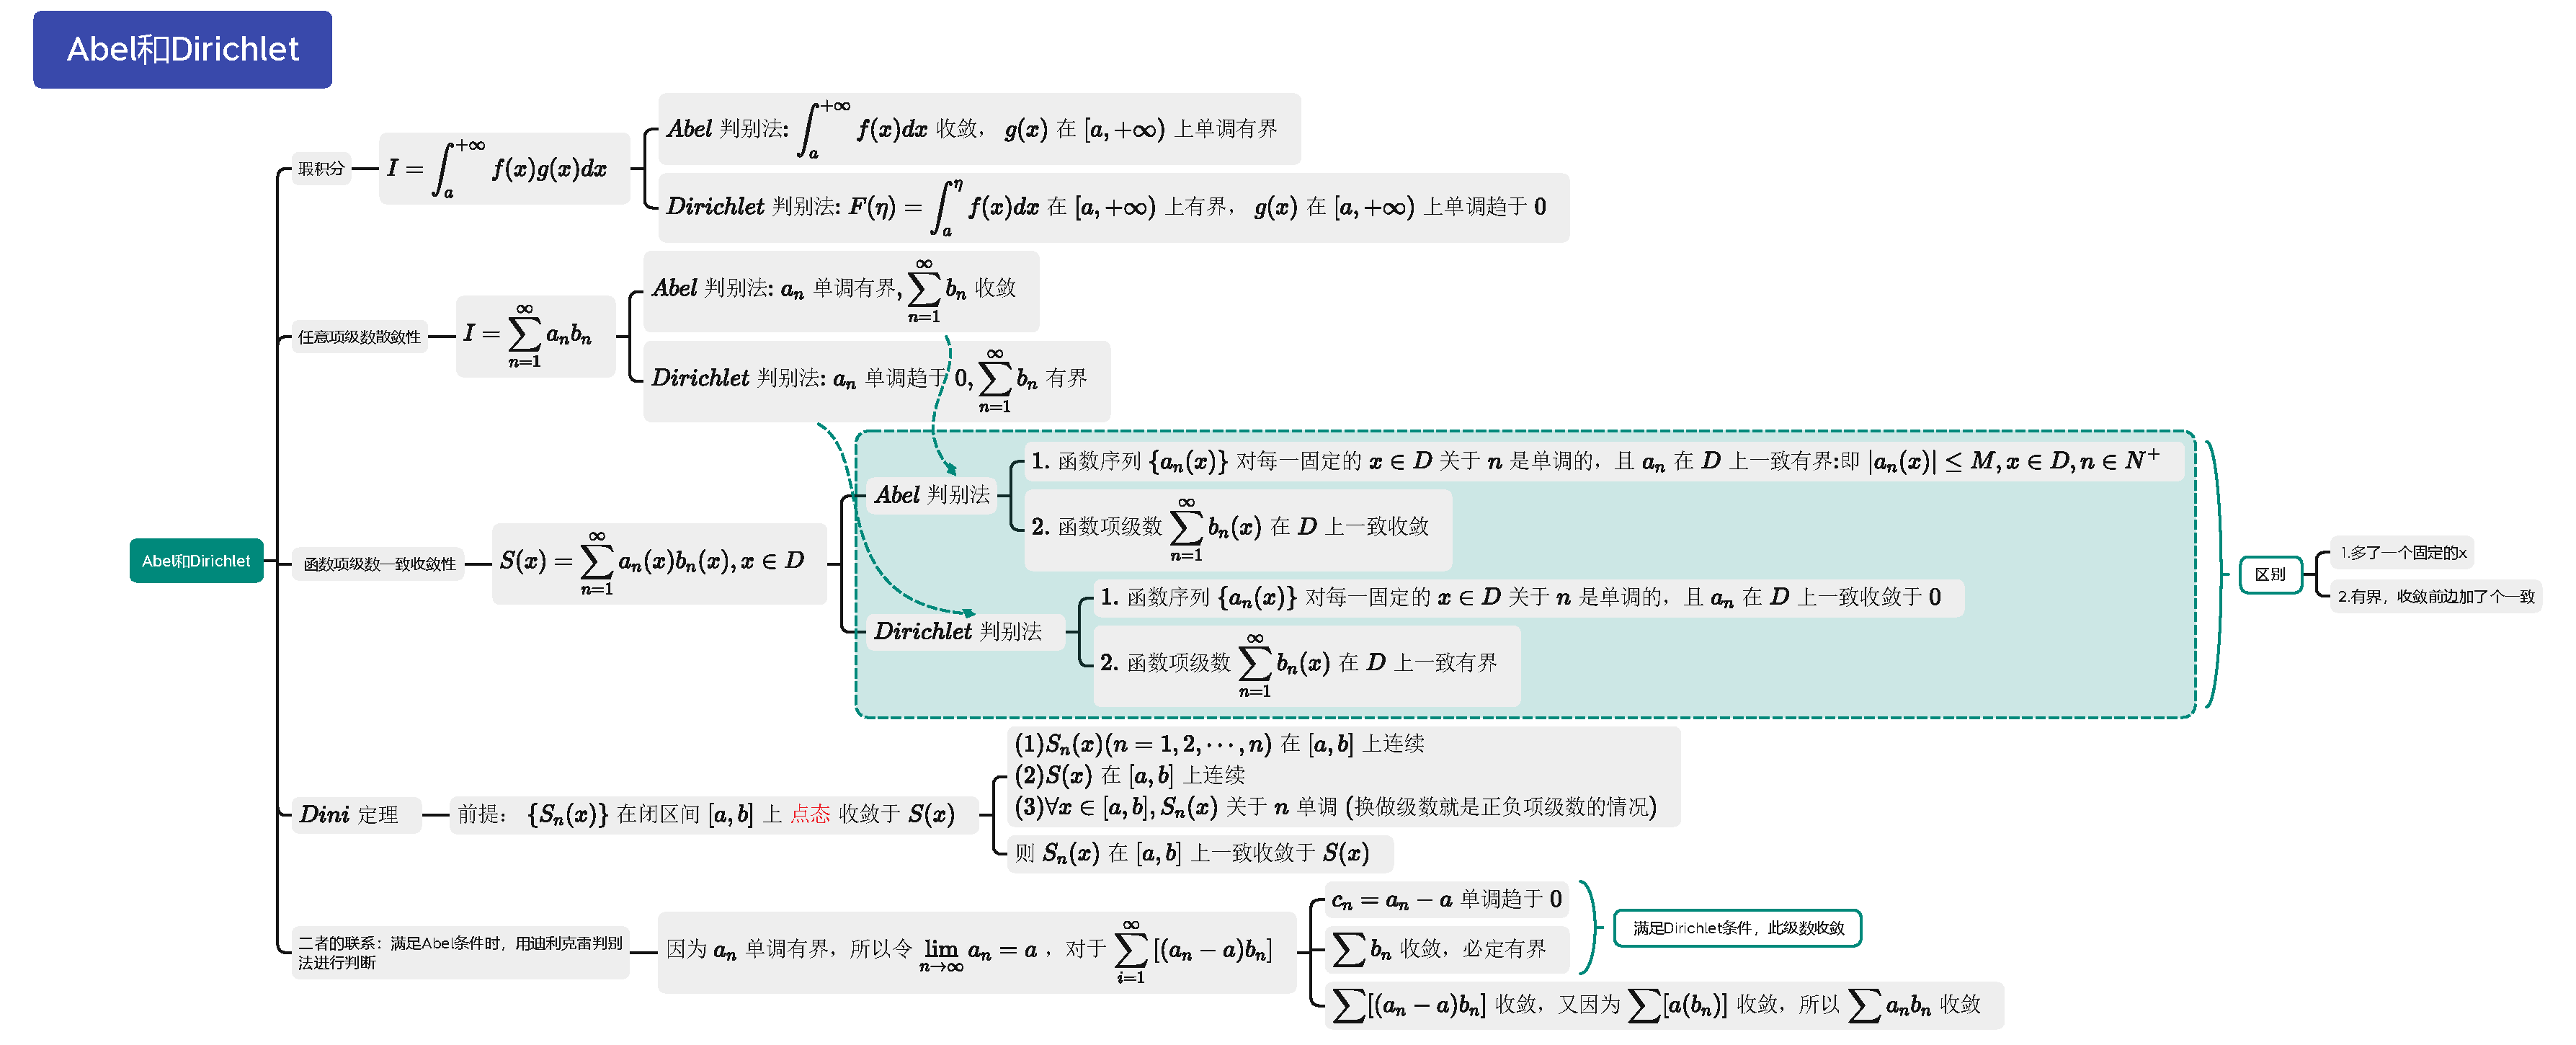
\includegraphics[scale=0.30]{Chapter/TikZ/Abel和Dirichlet.pdf}
    \label{Abel和Dirichlet}
    \caption{Abel和Dirichlet}
\end{figure}

那么判断级数的收敛性有什么作用呢?我们主要是应用它的如下性质:\par
\begin{figure}[!htb]
    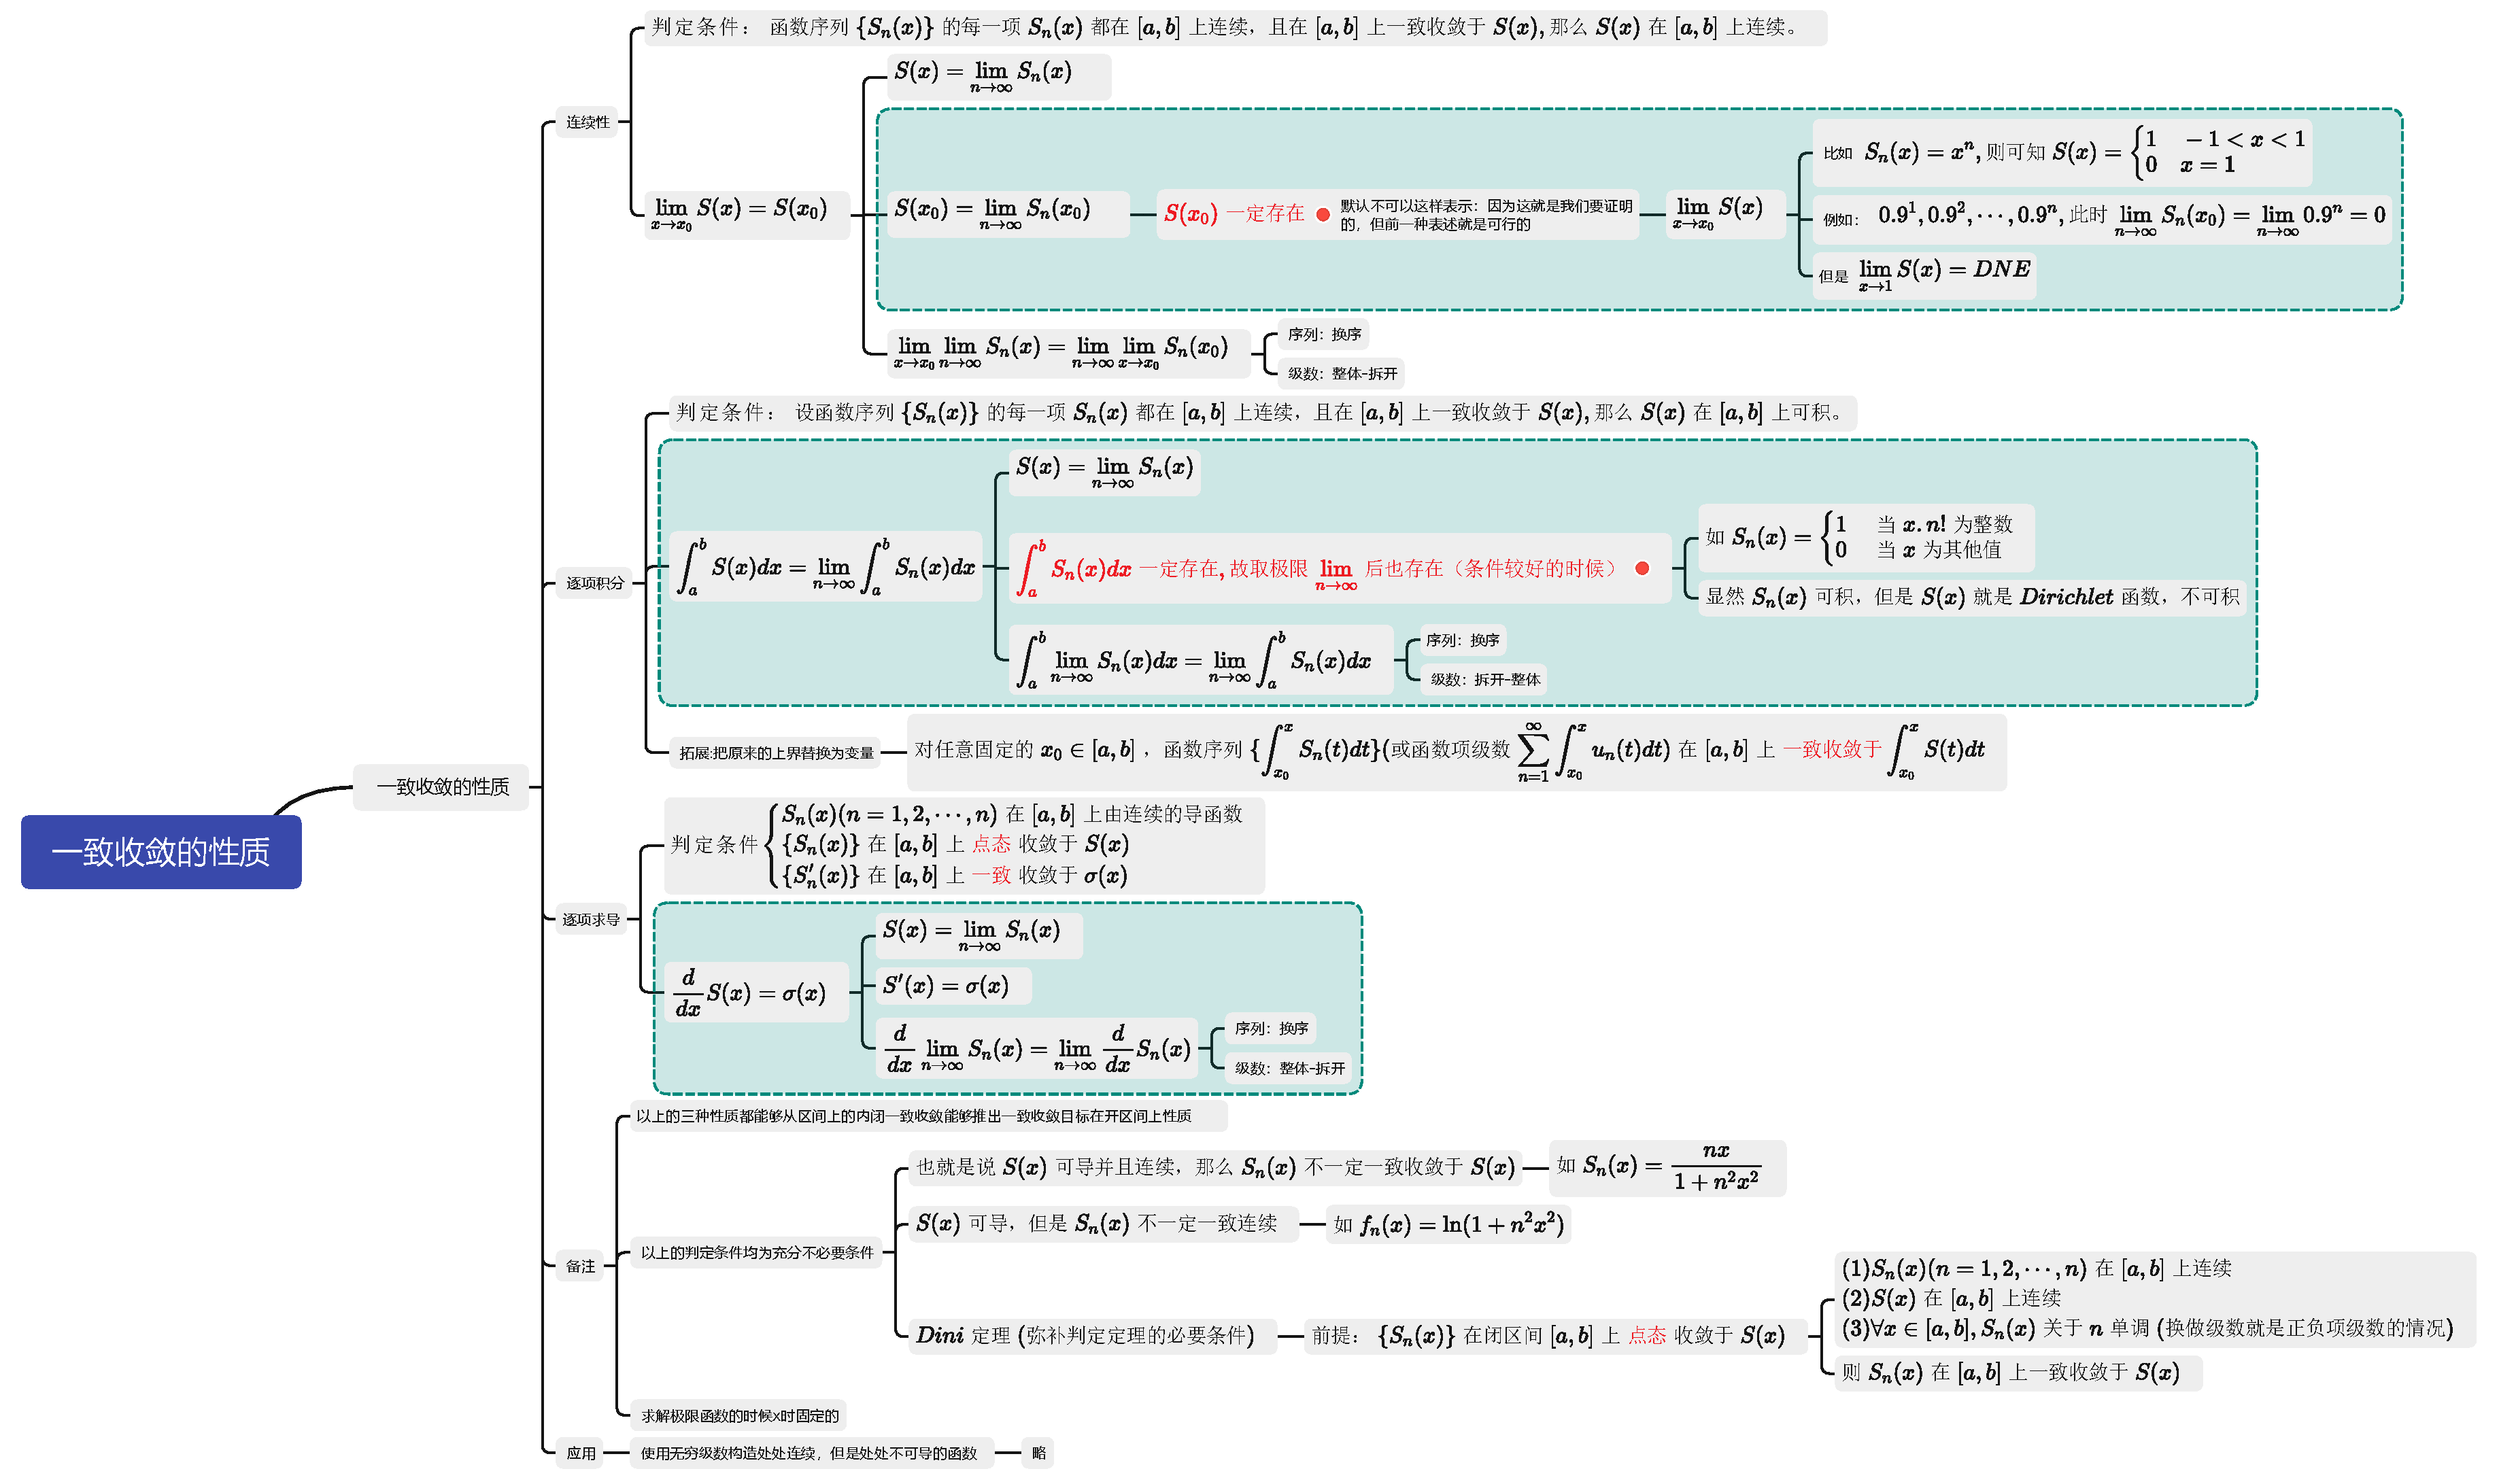
\includegraphics[scale=0.30]{Chapter/TikZ/一致收敛的性质.pdf}
    \label{一致收敛的性质}
    \caption{一致收敛的性质}
\end{figure}


\newpage
\section{极限}
\begin{definition}[极限定义]
    \textbf{\songti 函数极限的定义}\par
    $\forall \varepsilon>0, \exists \delta>0, 
    $当$|x-x_0|<\delta$时,~~ $\left|f(x)-f(x_0)\right|<\varepsilon$\par
    也就是说我的$f(x)$和$f(x_0)$可以无限接近,你要有多接近就有多接近,
    只要你给出接近的距离标准,比如 $0.1, 0.01, 0.001,\cdots$.我都有一个 $\delta$与之对应.\par
    
    \vspace*{2em}
    \textbf{\songti 它的逆否命题}\par
    $\forall \delta>0, \exists \varepsilon_0>0$
    当$\left|f(x)-f(x_0)\right|$时,~~$\left|x-x_0\right|>\delta$\par
    他的理解就恰恰和上边相反,你的$f(x)$和$f(x_0)$无法任意的接近,
    无论你的 $\delta$  取多么的小.$f(x)$和$f(x_0)$之间总会有一个无法跨越的最小距离 $\varepsilon_0$.
\end{definition}

\subsection{上,下极限}
上下极限的示意图

\begin{figure}[!htb]
    \centering
    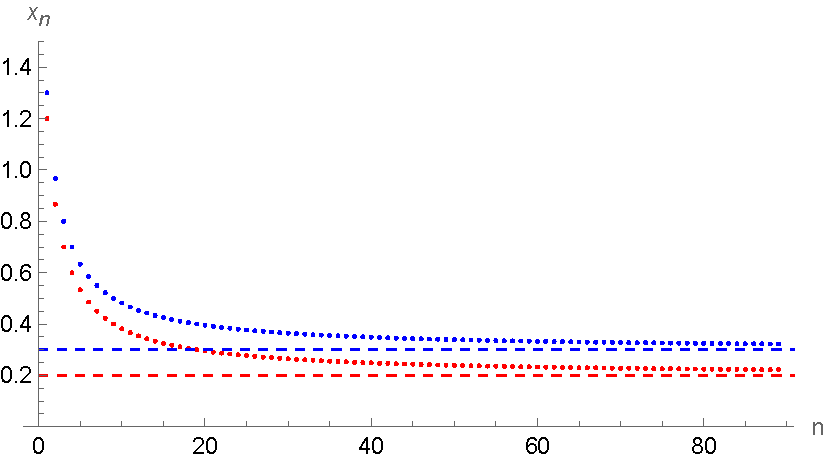
\includegraphics[scale=1]{Chapter/TikZ/上下极限散点图.pdf}
    \caption{上下极限散点图}   
\end{figure}



% 默认的行距是10pt
所有都$\ge$
$    
\begin{cases}
    \Longrightarrow \text{里边最小的都}\ge\\ 
    \Longrightarrow \text{里边的最大的也}\ge 
\end{cases}
\Longrightarrow x_n y_n \ge (H_1+\varepsilon)(H_2 + \varepsilon)
$


$\Longrightarrow \lim\limits_{n\to \infty}{x_ny_n} \ge \lim\limits_{n\to \infty}{(H_1+\varepsilon)(H_2 + \varepsilon)}$
$\Longrightarrow \lim\limits_{n\to \infty}{x_n y_n }\ge \lim\limits_{n\to \infty}{x_n}\cdot \lim_{n\to \infty}{y_n}$
问题在哪里?



    \subsection{函数极限的定义证明}
\newcommand{\Lim}[1]{\lim\limits_{x\to x_0}{#1}}


\noindent\textbf{等价性}

    证明:$\Lim{f(x)} = A \Leftrightarrow  \Lim{\left[f(x)-A\right]} = 0$

\begin{proof}

\textsf{1. 充分性}\par 
函数极限的定义: $\Lim{f(x)} = A$, 即 $\forall \varepsilon >0, \exists \delta>0$, 
当 $|x-x_0|<\delta$时, $|f(x)-A|<\varepsilon$\\
\bigskip
若有 $\Lim{[f(x)-A]} = 0$, 根据定义我们有:
$\forall \varepsilon>0, \exists \delta>0, \mbox{当}|x-x_0|<\delta$ 时:
\[
    |g(x) -0|= |(f(x)-A)-0|=|f(x)-A|<\varepsilon
\]
上面就是函数 $f(x)$ 极限的定义了。 注:把 $f(x)-A$看作 $g(x)$

\textsf{2. 必要性}\par 
若 $\Lim{f(x)} = A$, $\forall \varepsilon>0, \exists \delta>0, \mbox{当}|x-x_0|<\delta$
\[
    |f(x)-A| = |(f(x)-A) -0| = |g(x) -0|< \varepsilon
\] 
上面就是函数 $g(x) = f(x)-A$ 极限的定义了。
\textsf{证毕}
$\square$
\end{proof}

\noindent\textbf{和的极限}

\noindent 假设函数 $f(x), g(x) \mbox{在} x=x_0 $出的极限存在, 分别为 $A, B$.
证明: $\Lim{[\alpha f(x)+\beta g(x)]} = \alpha A + \beta B$

\begin{proof}

    $\forall \varepsilon>0, \exists \delta>0, \mbox{当}|x-x_0|<\delta$ 时:
    因为 $f(x), g(x)$在 $x=x_0$处均极限存在.所以在此条件($|x-x_0|<\delta$)下我们有:
\begin{align*}
    & | f(x) |< X\\
    & |f(x)-f(x_0)| <\frac{\varepsilon}{2A} \\
    & |g(x)-g(x_0)| <\frac{\varepsilon}{2B}
\end{align*}
于是我们有:
\begin{align*}
    |(\alpha f(x)+\beta g(x)) - (\alpha f(x_0)+\beta g(x_0))| 
    &= |\alpha\cdot(f(x)-f(x_0)) + \beta\cdot(|g(x)-g(x_0)|)| \\
    & \le \alpha\cdot|f(x)-f(x_0)| + \beta\cdot|g(x)-g(x_0)|\\
    & \le A\cdot\frac{\varepsilon}{2A} + B\cdot\frac{\varepsilon}{2B}\\
    & < \varepsilon  
\end{align*}
\textsf{证毕}
$\square$

\textsf{注:函数乘积的极限证明同理}\par 
\[
    | f(x)g(x)-AB|=| f(x)(g(x)-B)+B(f(x)-A)|<(X+ |B|)\varepsilon'  
\]
$\varepsilon'$的构造和上面同理

\end{proof}
    \section{定积分与黎曼和}
\begin{definition}
    设$f(x)$是定义在$[a,b]$上的有界函数,在$[a, b]$上任取分点$\{x_i\}^n_{i=0}$,做一种划分:
    \[
        P:a=x_0<x_1<x_2<\cdots<x_{n-1}<x_n=b
    \]
    并且任取点$\xi_i\in[x_{i-1},x_i]$.记小区间的长度为$\Delta x_{i-1}=x_i-x_{i-1}$,并令$\lambda=\max\limits_{1\le i\le n}(\Delta x_i)$,若当$\lambda\to 0$时,极限
    \begin{equation}
        \lim\limits_{\lambda\to 0}{\sum_{i}^{n}{f(\xi_i)\Delta x_i}}\nonumber
    \end{equation}
    存在,并且与划分P无关,又对$\xi_i$的取法无关,则称$f(x)$在$[a, b]$上Riemann可积,和式
    \begin{equation}
        S_n= \sum_{i=1}^{n}{f(\xi_i\Delta x_i)}\nonumber
    \end{equation}

    称为Riemann和,其极限$I$称为$f(x)$在$[a, b]$上的定积分,记为:
    \begin{equation}
    I=\int_{a}^{b}{f(x) \dd x}\nonumber
    \end{equation}
\end{definition}
下边给出几个基本的求取范例,其实本质思想都是相同的\\
\vspace*{3pt}


\begin{framed}
    \begin{align*}
        & I_1=\int_{a}^{b}{e^x \mathrm{d}x}
        & \displaystyle I_2= \int_{a}^{b}{x^2 \mathrm{d}x}
    \end{align*}
\end{framed}

\begin{formal}{blue!20}
    对于是否Riemann可积,其实就是需要我么们去计算积分的上限和下限。
\end{formal}

\begin{proof}\textsf{第一题}

对于积分上限,我们需要计算的表达式即为:
\[
    \lim_{n\to\infty}{\frac{b-a}{n}e^a\cdot \sum_{i=1}^{n}{e^{\frac{i\cdot(b-a)}{n}}}}\nonumber \\
\]

\begin{align*}
    {\rm LSH}
    &=\lim_{n\to\infty}
    {
        e^a\cdot\frac{b-a}{n}\frac{e^{\frac{b-a}{n}}[1-e^{\frac{b-a}{n}\cdot n}]}{1-e^{\frac{b-a}{n}}}
    }
    =\lim_{n\to\infty}
    {
        e^a\cdot\frac{b-a}{n}\cdot\frac{e^{ \frac{b-a}{n} }[e^{b-a}-1]}{\lim\limits_{n\to\infty}{   e^{  \frac{b-a}{n} }   }-1}
    }\\
    &=\lim_{n\to\infty}
    {
        e^a\cdot\frac{b-a}{n}\cdot
        \frac{e^{\frac{b-a}{n}}[e^{b-a}-1]}  {\frac{b-a}{n}}
    }
    =\lim_{n\to\infty}
    {
        e^a\cdot e^{\frac{b-a}{n}}\cdot[e^{b-a}-1] 
    }\\
    &=e^b-e^a
\end{align*}   


对于积分下限,我们需要计算的表达式即为:
\[
    \lim_{n\to\infty}{\frac{b-a}{n}e^a\cdot \sum_{i=1}^{n}{e^{\frac{(i-1)\cdot(b-a)}{n}}}}\nonumber
\]


\begin{align*}
    {\rm LSH}
    &=\lim_{n\to\infty}
    {
        e^a\cdot\frac{b-a}{n}\frac{e^{0}[1-e^{\frac{b-a}{n}\cdot n}]}{1-e^{\frac{b-a}{n}}}
    }
    =\lim_{n\to\infty}
    {
        e^a\cdot\frac{b-a}{n}\cdot
        \frac{e^{0}[e^{b-a}-1]}  {\frac{b-a}{n}}
    }\\ 
    &=\lim_{n\to\infty}
    {
        e^a\cdot e^{0}\cdot[e^{b-a}-1] 
    }
    =e^b-e^a\nonumber
\end{align*}

由此我们可以得出,积分上限和积分下限相等,所以Riemann和为:
\[
I_1=e^b-e^a
\]
\end{proof}


\begin{proof}\textsf{第二题}

首先做分割,$T=\{a, a+\frac{a-b}{n}, \cdots, a+\frac{(n-1)(b-a)}{n}, b\}$, 并取$\xi_i=$,此时的Riemann和为:

\begin{align*}
    I_2 
    & = \int_{a}^{b}{\frac{1}{x^2} \dd x}
        = \lim_{n\to\infty}{\sum_{i=1}^{n}{f(\xi_i)\frac{a-b}{n}}}\\
    & = \lim_{n\to\infty}{\sum_{i=1}^{n}{f(\xi_i)}}
\end{align*}
    
因为$\xi_i\in [x_{i-1}, x_i]$ 而且要求 $f(\xi_i)$ 作为通项,
要便于我们求和,即 $\frac{1}{\xi_i^2}$ 便于求和.
考虑到 $\frac{1}{2\times 3}=\frac{1}{2}-\frac{1}{3}$ ,受到启发,
所以我们便取 $\xi_i=\sqrt[]{x_{i-1}x_i}$ 的形式, 所以我们取
\begin{align*}
    \xi_i=\sqrt[]{[\frac{(i-1)(b-a)}{n}+a]\cdot[\frac{i\cdot(b-a)}{n}]}
\end{align*} 


C为一个待求解的常数。因为 $na+i(a-b)-na-(i-1)(a-b)=a-b\Longrightarrow {\rm C}=\frac{1}{a-b}$, 所以我们可以得到:
\begin{align*}
    C = \frac{1}{a-b}
\end{align*}

带入原式我们有:
\begin{align*}
    \mathrm{LHS} 
    & = \int_{a}^{b}{ \frac{1}{x^2}\dd x}=\lim_{n\to\infty}{\frac{a-b}{n}\sum_{i=1}^{n}{\frac{1}{x_{i-1}x_i}}}
      = \lim_{n\to\infty}{\frac{a-b}{n}\sum_{i=1}^{n}{{\rm C}\cdot[\frac{1}{a+\frac{(i-1)(a-b)}{n}}-\frac{1}{a+\frac{i\cdot(a-b)}{n}}]}}\\
    & = \lim_{n\to\infty}{\frac{1}{a-b}\cdot (a-b)\sum_{i=1}^{n}{[\frac{1}{a+\frac{(i-1)(a-b)}{n}}-\frac{1}{a+\frac{i\cdot(a-b)}{n}}]}}
      = \sum_{i=1}^{n}{[\frac{1}{na+(i-1)(a-b)}-\frac{1}{na+i\cdot(a-b)}]}\\
    & = \lim_{n\to\infty}\sum_{i=1}^{n}[(\frac{1}{na+0(a-b)}-\frac{1}{na+(a-b)})+(\frac{1}{na+(a-b)}-\frac{1}{na+2(a-b)})\\
    & \quad+\cdots+(\frac{1}{na+(n-1)(a-b)}-\frac{1}{na+n(a-b)})]\\
    & = \lim_{n\to\infty}{[\frac{1}{na+0(a-b)}-\frac{1}{na+n(a-b)}]}
      =\lim_{n\to\infty}{[\frac{1}{n}(\frac{1}{a}-\frac{1}{2a-b})]} = 0
\end{align*} 

有错,之后再检查检查!!
\end{proof}
    \newpage
\section{实数基本定理}
这六个定理虽然出发的角度不同,但是都是描述实数连续性这同一回事,他们之间是相互等价的,
即任取其中两个定理,他们可以相互证明。他们在证明过程中相互联系。对同一个定理的证明,
虽然不同的定理作为工具会使证明有简繁之分,有的用的是类似的证明方法,有的出发点与站的角度不同,
但最后却能殊途同归。而有时使用同一个定理,也可能有不同的方法。即是方法相同,也有可能有不同的细节。
作为工具,他们又各具特点。而这些都是值得我们去注意与发现的!   

\vspace*{1em}
\begin{theorem}[实数基本定理]
    \noindent\ding{172} 确界存在定理:非空有上 (下)界数集,必有上 (下)确界。%英文字符和中文字符之间加一个空格不会警告

    \noindent\ding{173} 单调有界收敛原理:任何单调有界数列必有极限。

    \noindent\ding{174} 区间套定理:若$\{\left [ a_n,b_n \right ]\}$是一个区间套,则存在唯一一点$\xi$,使得$\xi\in \left [ a_n,b_n \right ] ,n=1,2,\cdots $

    \noindent\ding{175} \textit{Heine-Borel}有限覆盖定理:设$\left [ a,b \right ]$是一个闭区间,H为$\left [ a,b \right ]$的一个开覆盖,则在H中
    存在有限个开区间,它构成$\left [ a,b \right ]$上的一个覆盖。

    \noindent\ding{176} \textit{Weierstrass}聚点定理 (\textit{Bolzano}致密性定理:有界无穷数列必有收敛子列):直线上的有解无限点集至少有一个聚点。

    \noindent\ding{177} \textit{Cauchy}收敛准则:数列$\{a_n\}$收敛 $\Longleftrightarrow$对任给定的正数$\varepsilon$,总存在某一个自然数$N$,使得$\forall m,n>N$时,
    都有$\left| a_m-a_n \right| < \varepsilon\Longleftrightarrow \{a_n\}$ 是基本数列。
\end{theorem}

\begin{proof}
如图所示
\begin{center}
    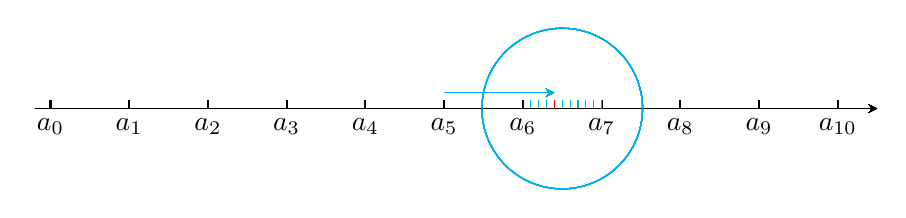
\begin{tikzpicture}[>=stealth]
        \foreach \i in {0, 1, ..., 10}
        {
            \draw[ ->] (-0.2, 0)--(10.5, 0);
            \draw[cyan] (6+\i/10, 0)--(6+\i/10, 3pt);
            \draw[red] (6.4, 0)--(6.4, 3pt);
            \draw[thick] (\i, 0)node[below]{$a_{\i}$}--(\i, 3pt);
            \draw[cyan] (6.5, 0) circle [radius=1.02];
            \draw[->, cyan] (5, 0.2) -- (6.4, 0.2);
        }
    \end{tikzpicture}
\end{center}
\end{proof}

\clearpage
    \section{平面点集}


\subsection{孤立点和界点}

孤立点一定是界点,为什么呢?这就意味着, 孤立点的任何邻域里边一定有不含于E的点?
但是这个去心邻域可能是空的,哪里来的不属于E的点呢?


\begin{figure}[!htb]
    \begin{minipage}[b]{0.3\linewidth}
        \num{1}\quad $U$为全集\\[2em]
        \num{2}\quad $E$为所求集合\\[2em]
        \num{3}\quad $E^C$为$E$的补集
    \end{minipage}
    \hfill
    \begin{minipage}[t]{0.6\linewidth}
        % 注释掉的内容为原本的tikzit绘图
        % \vspace*{1pt}
        % \ctikzfig{Chapter/TikZ/Boundaries}
        % \caption{界点图解}
        \centering
        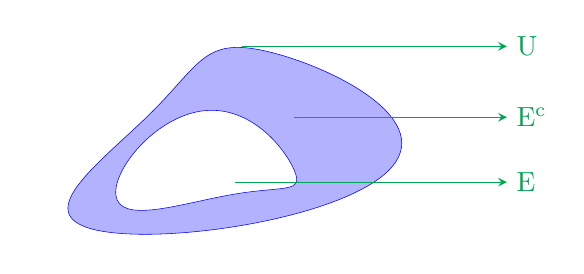
\begin{tikzpicture}[scale=1.5]
            \definecolor{Green}{HTML}{00a652}
            \begin{scope}
                \draw[very thin, fill=Blue!30, draw=Blue] %
                    plot [smooth cycle, tension=1] %
                    coordinates {(1.5, 2.5) (4, 3) (3, 4) (2, 3.5)};       
            \end{scope}
            \begin{scope}[shift={(1.2, 1.5)}]
                \draw[very thin, fill=white, draw=Blue] %
                    plot [smooth cycle, tension=1] % 
                        coordinates {(0.5, 1.25) (1.5, 1.3) (2, 1.5) (1.2, 2)};
            \end{scope}
            \begin{scope}[shift={(2, 3)}]
                \draw[->, >=stealth, Green] (0.7, -0.1)--(3, -0.1)node[right]{$\mathrm{E}$}; 
                \draw[->, >=stealth, Green] (1.2, 0.45)--(3, 0.45)node[right]{$\mathrm{E^c}$}; 
                \draw[->, >=stealth, Green] (0.76, 1.05)--(3, 1.05)node[right]{$\mathrm{U}$}; 
            \end{scope}
        \end{tikzpicture}
        \caption{界点图解}
        \label{界点图解}
    \end{minipage}
\end{figure}

\subsection{上确界存在定理}
% \begin{figure}[!htb]
%     \ctikzfig{Chapter/TikZ//Supremum}
%     \caption{确界直观理解图}
% \end{figure}


我们令 $a_i = a_{{(i-1)}_{10}} = a_{{i}_0}$, $[a_0, a_{10}]$的长度为 $1$,于是可以得到
$a_6 = 0.6 = a_7 - \frac{1}{10},a_7 = 0.7$.把区间放大之后:
区间 $[a_{6_0}, a_{6_{10}}]$的长度为 $\frac{1}{10}$, 于是可以得到
$a_{6_6} = a_{6_7} - \frac{1}{10^3} = a_6 + 7\cdot\frac{1}{10^2}-\frac{1}{10^3}, a_{6_7} = 0.67$.\
然后一直这样迭代下去,根据实数的十进制表示方法可以知道这样的 $\sup\mathrm{E}$是存在且唯一的。

\begin{figure}[!htb]
    \begin{tikzpicture}
        \centering
        \begin{scope}[>=stealth, scale=0.8]
            \foreach \i in {0, 1, ..., 10}
            {
                \draw[ ->] (-0.2, 0)--(10.5, 0);
                \draw[cyan] (6+\i/10, 0)--(6+\i/10, 3pt);
                \draw[red] (6.4, 0)--(6.4, 3pt);
                \draw[thick] (\i, 0)node[below]{$a_{\i}$}--(\i, 3pt);
                \draw[cyan] (6.5, 0) circle [radius=1.02];
                \draw[->, red] (5, 0.2) -- (6.4, 0.2);
            }
        \end{scope}
        \draw[->] (5.12, 0)--(5.12, -2.4)--(6, -2.4);
        % 5.12 = 6.4*0.8,   2.4 = 3*0.8
        \node[below] (A) at (5.12, -1.2) {把这个小区间放大10倍};
        \node[left] (B) at (4, 0.2) {$\sup\mathrm{E}$};
        \begin{scope}[>=stealth, scale=0.8, shift={(8, -3)}]
            \foreach \i in {0, 1, ..., 10}
            {
                \draw[ ->] (-0.2, 0)--(10.5, 0);
                \draw[cyan] (6+\i/10, 0)--(6+\i/10, 3pt);
                \draw[red] (6.4, 0)--(6.4, 3pt);
                \draw[thick] (\i, 0)node[below]{$a_{6_{\i}}$}--(\i, 3pt);
                \draw[cyan] (6.5, 0) circle [radius=1.02];
                \draw[->, red] (5, 0.2) -- (6.4, 0.2);
            }
        \end{scope}
        \node[left] (C) at (10.4, -2.24) {$\sup\mathrm{E}$};
        % 10.4 = (5+8)*0.8,  2.24 = (3-0.2)*0.8
    \end{tikzpicture}
    \caption{确界直观理解图}
\end{figure}

\subsection{内闭一致收敛}
我们都知道函数列一致收敛的几何意义:就是当$n$充分大后的函数曲线系能够都落在关于
极限函数的一个带形区域内(宽为$2\varepsilon$)。
现在你要检查某个区间上函数列是否一致收敛,形象地讲,
闭区间的端点就是你要考虑的范围、限度,
出了这个界你就不考虑这个界以外的曲线能否落在你所预设好的带形区域内。那么,
假设你已经知道在闭区间I上的某个函数列是内闭一致收敛的,
并且很恰巧地你注意到n必须要非常非常大比如$n=1000$,你的这个函数列的曲线系
才开始勉强落入带形区域。
(这种极端情况正是接下来内闭一致收敛不是一致收敛的重要原因。)然后,
你把闭区间$I$向外扩充一点点变成一个开区间$D$,于是,
完全可能出现这样一种情况:$n=1000$已经不能让函数曲线们落入带形区间里了,
你把$n$不断扩大,可是不管$n$怎么大,
开区间的端点附近的$x$点总能找出一部分能让你的曲线系落到带形区间外,
而且你没法定死最无法使你的曲线系落入带形区间的x点以便你能找到最大的$n$,
因为这是开区间!端点处附近永远存在一部分点当你自以为找到足够大的$n$后让
你的曲线系落到带形区间外。
这就是某些内闭一致收敛不一定一致收敛例子的几何解释


\begin{figure}[!htb]
    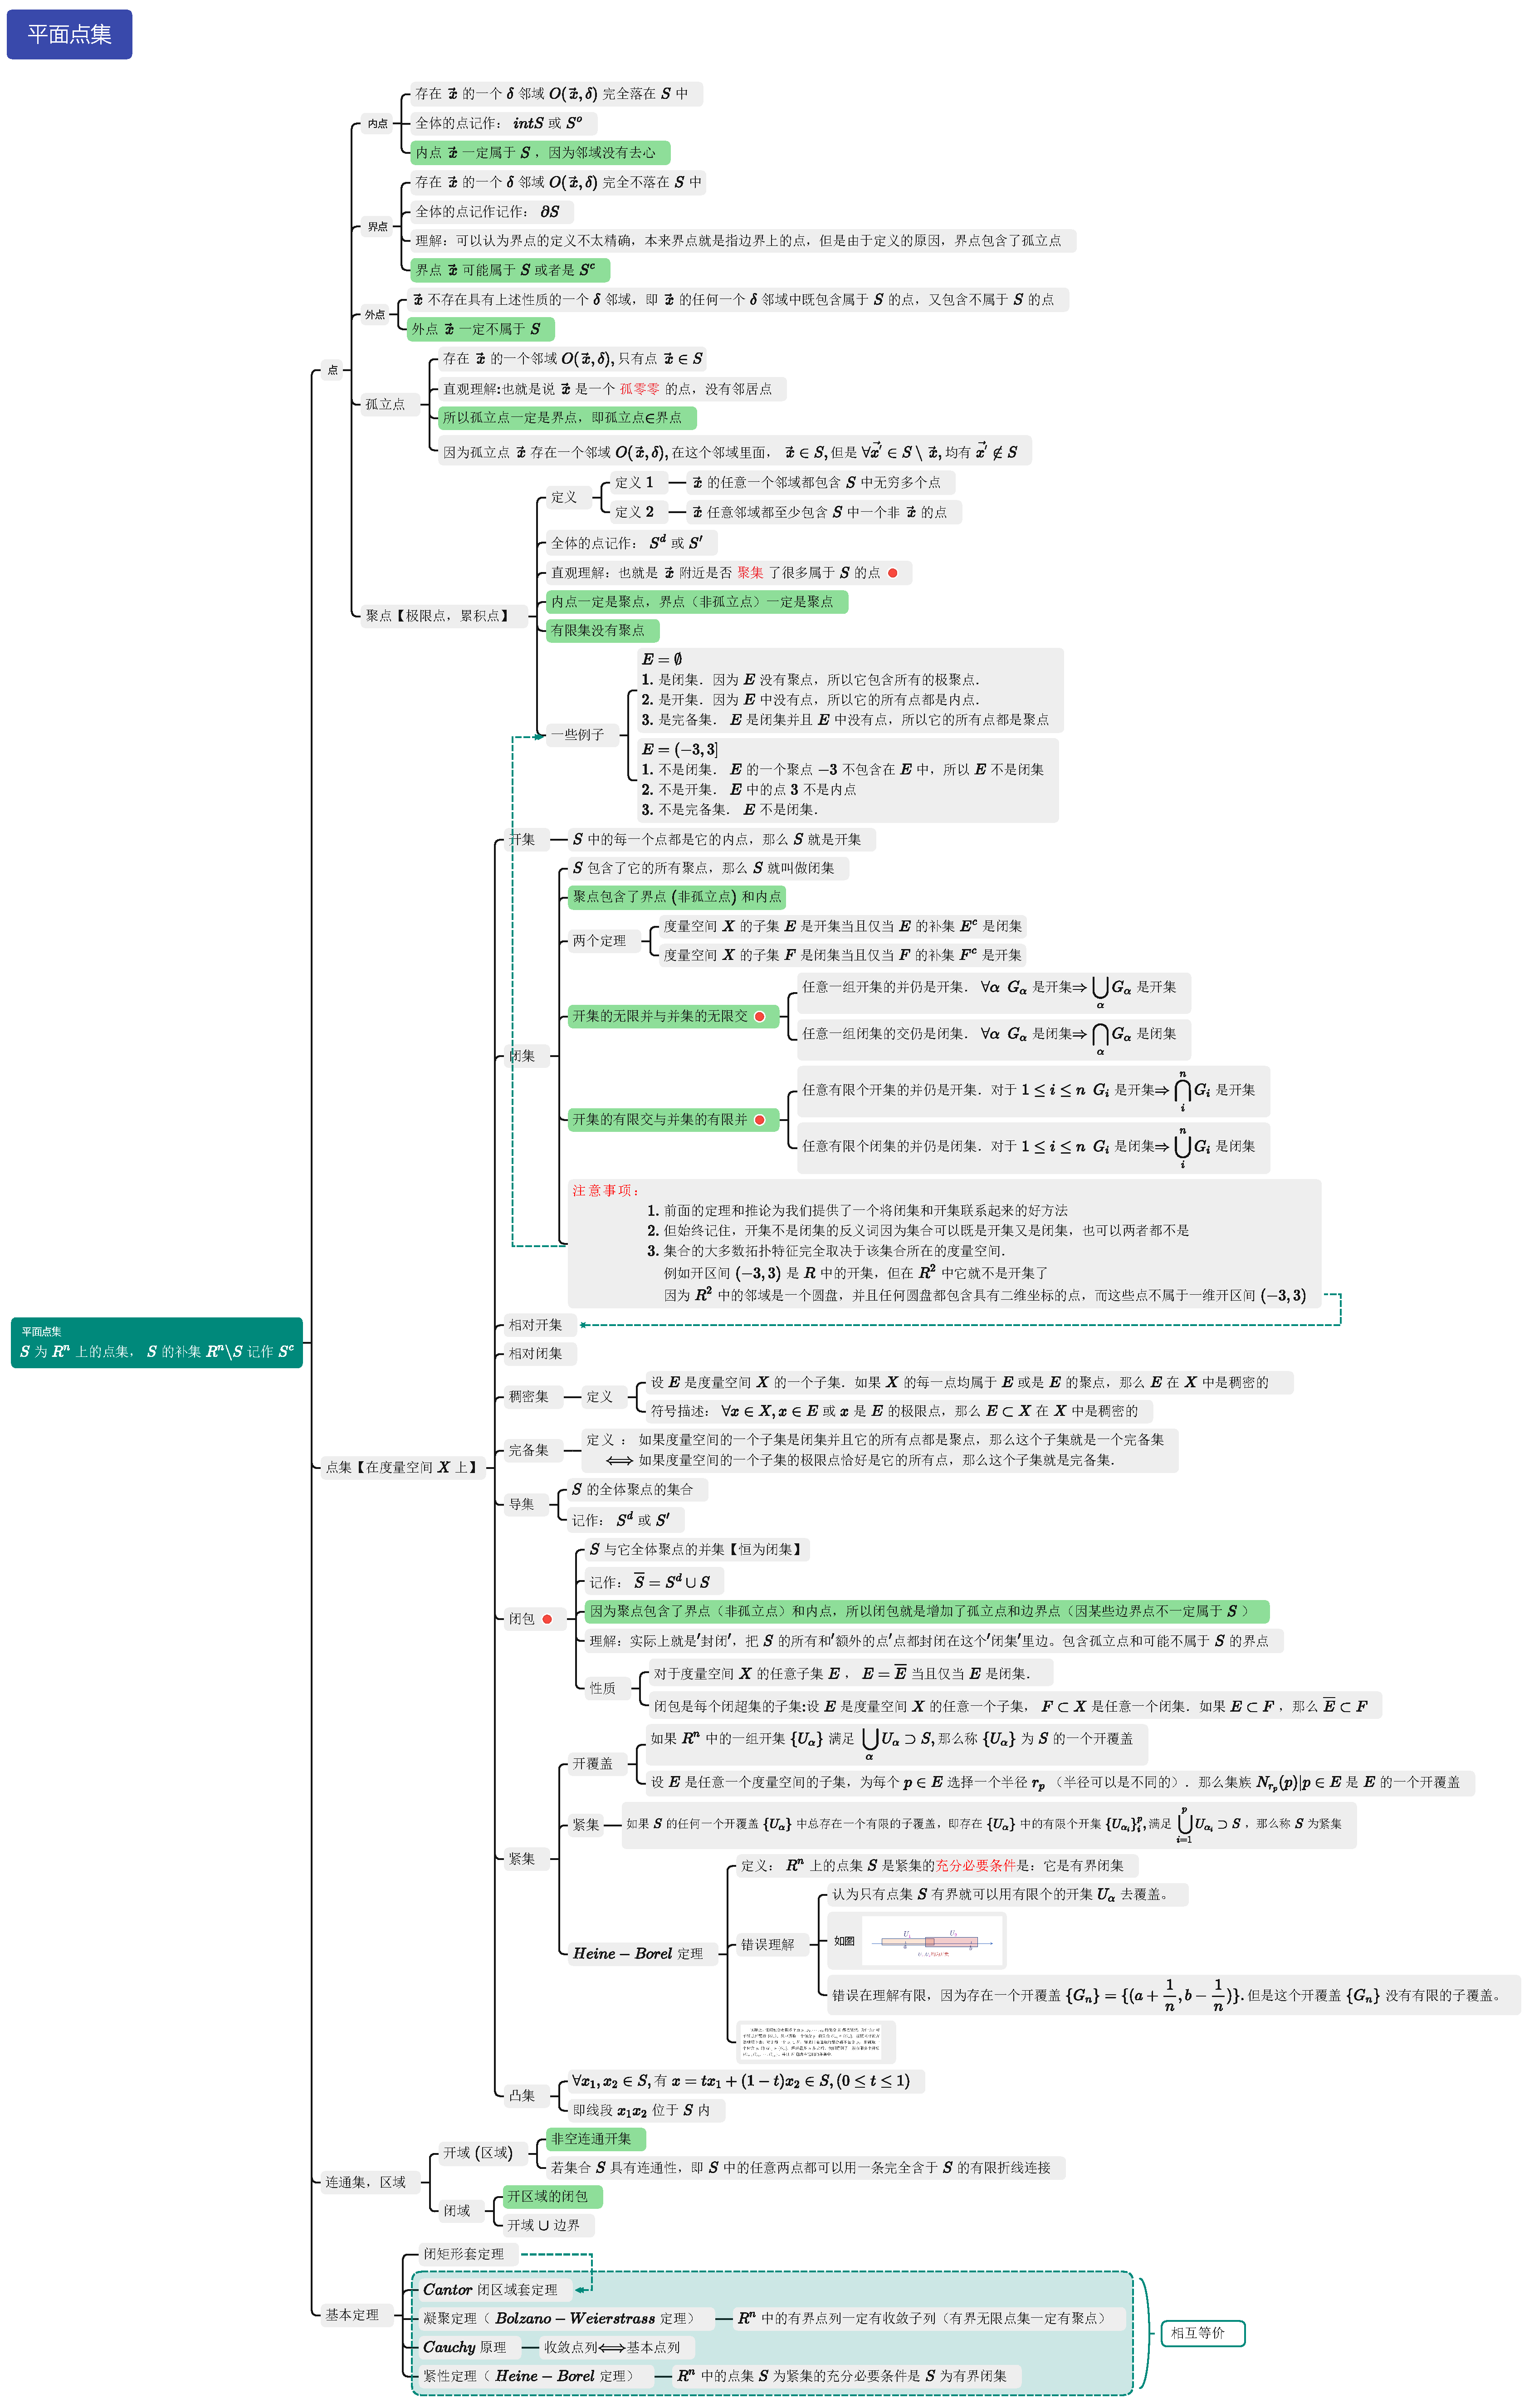
\includegraphics[scale=0.3]{Chapter/TikZ/平面点集.pdf}
    \label{平面点集}
    \caption{平面点集}
\end{figure}
    \section{Fourier级数}

主要是研究函数的傅里叶展开式,本章的知识逻辑关系图如下,
\begin{figure}[!htb]
    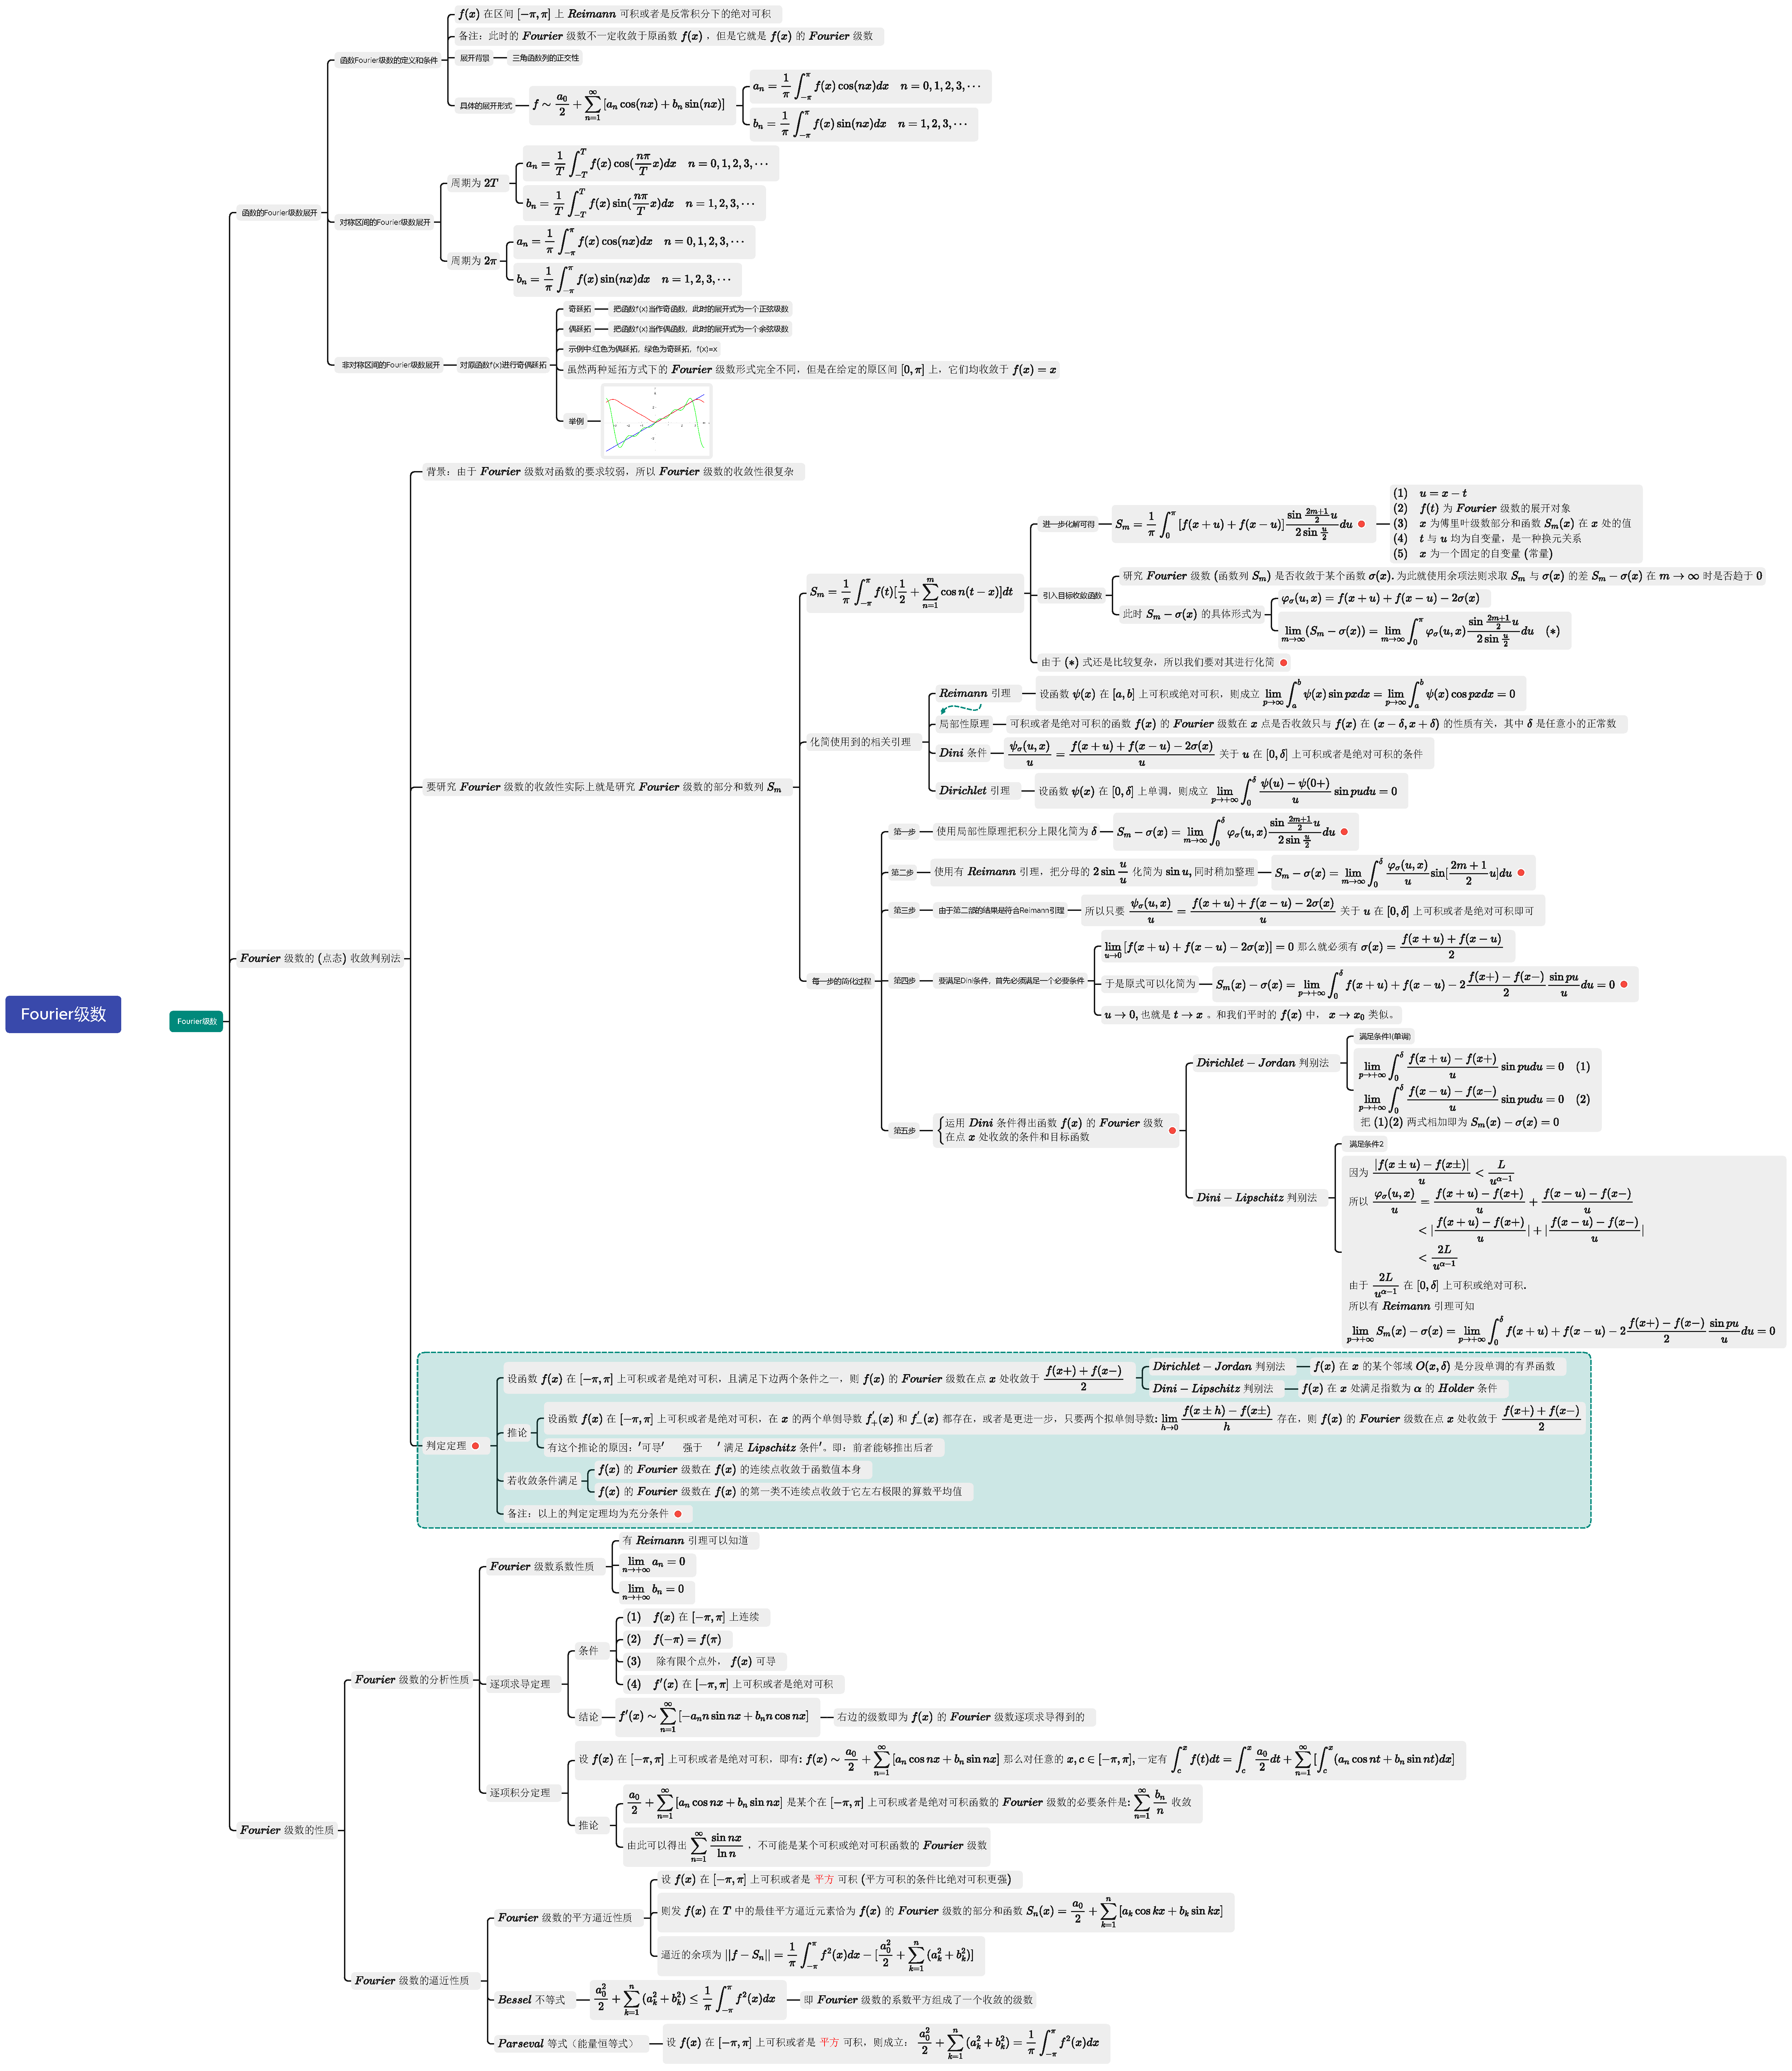
\includegraphics[scale=0.2]{Chapter/TikZ/Fourier级数.pdf}
    \label{Fourier级数}
    \caption{Fourier级数}
\end{figure}


    \chapter{Algebra}
    \section{线性代数}
\subsection{线性相关}

$x^{2}$与$x|x|$在$C[-1,1]$是否线性相关?

\begin{proof}

    $c_{1} x^{2}+c_{2} x|x|=0 $, 
    在 $[0,1]$上$c_{1}=1,c_{2}=-1$,
    在 $[-1,0]$上$c_{1}=1,c_{2}=1$,
    所以它们在$C[-1,1]$是线性相关的. 
\end{proof}

\subsection{矩阵转置} 
\begin{align*}
    R =\begin{bmatrix}
        A\\
        B
    \end{bmatrix}
    \Longrightarrow
    R^T=\begin{bmatrix}
        A^T\\
        B^T
    \end{bmatrix}^T 
    = \left[A^T, B^T\right]
\end{align*}

\subsection{左行右列}
其实可以看做是,行列式的最左边乘以一个运算,这个运算是第二行减去第一行的$A$倍。
由此我们可以看出:分块矩阵也是符合左行右列的规则的。
\begin{align*}
    \left|
        \begin{matrix}
            E & O\\ 
            -A & E
        \end{matrix}
    \right|
    \cdot 
    \left|
        \begin{matrix}
            E & B\\ 
            A & E 
        \end{matrix}
    \right|
    = \left|
        \begin{matrix}
            E & B \\ 
            O & E - AB 
        \end{matrix}
    \right|
\end{align*}

\subsection{过渡矩阵}

\[AX = BY\]

因为$A\to B$的过度矩阵为$P = A^{-1}B$。
举例:令前后的基为$\{\xi_1 = 4, \xi_1^{'} = 2\}$, 一个向量在变换前后的坐标分别为$b_1 = 5, b_1^{'} = 10$
因为$4\times 5 = 2\times 10$,可以认为是基从$5\to10$,这个坐标变换就是$p^{-1} = \frac{1}{2}x$.所以我们可以知道基变换
就是$P = 2x$

\subsection{向量空间}
比如 $\mathrm{A}$ 有特征值 $\lambda_i$, 对应的特征向量为 $\mathrm{p}_i$
我把 $\mathrm{p}_i$ 正交化后的得到的正交基记为 $\xi_i$

疑问一: 那么 $\xi_i$ 是对应于 $A$ 的特征值为 $\lambda_i$ 的特征向量吗? 

疑问二:为什么$p_i$单位正交化后的$\xi_i$, 
\begin{align*}
    \xi 
    & = \biggl(\xi_1,\, \xi_2,\, \xi_3,\, \cdots,\, \xi_i\biggr)
      \Longrightarrow  A=\xi^T \operatorname{diag}\left(\lambda_1, \lambda_2, \cdots, \lambda_i\right) \xi
\end{align*}

\begin{proof}

当 $\mathrm{A}$ 是对称实矩阵时, 只有当 $\lambda_i$ 为重根时才需要对求出的特征向量正交化, 且正交化后的向量仍然是原矩阵的特征向量。

如 $\lambda_i$ 为二重根, 则有 $\mathrm{p}_1, \mathrm{p}_2$ 两个特征向量与之对应。
正交化后即有,
\begin{align*}
    \xi_i=p_1, \xi_2=p_2-\frac{[p_1,\xi_1]}{[\xi_1,\xi_1]}\xi_1=p_2-kp_1
\end{align*}

故 
\begin{align*}
    A \xi_2
    & = A\left(\mathrm{p}_2-k p_1\right)=A p_2-k A p_1 \\
    & =\lambda_i p_2-k \lambda_i p_2 = \lambda_i\left(\mathrm{p}_2-k p_1\right)
\end{align*}
当 $A$ 不是对称矩阵时, 正交化后的向量就不是原矩阵的特征向量.至于为何是这样的结构, 记住!
\end{proof}

\subsection{线性空间相关问题}
线性空间V上的所有线性变换所组成的线性空间$\tau$。那么$\tau$里边的所有元素
对V中的所有元素所用后还在V中吗?

怎么求线性空间的零元素?

\subsection{特征值问题}
\begin{theorem}[特征值的性质]
\begin{align}
    \prod_{i=1}^n \lambda_i=|A|\hspace*{0.3\linewidth}\sum_{i=1}^n a_{i i}=\sum_{i=1}^n \lambda_i
\end{align}
\end{theorem}

\begin{proof}

    \num{1} 从特征多项式考虑:若关于矩阵A的特征多项式 $f(\lambda)$ 有根:
    $\lambda_1, \lambda_2, \cdots, \lambda_n$.(可能有重根,但是不影响)

    那么根据代数学基本定理可以知道, 若关于矩阵A的特征多项式可以分解为:
    \begin{align*}
        |\lambda E - A|&=f(\lambda)=\left(\lambda-\lambda_1\right)\left(\lambda-\lambda_2\right) \cdots\left(\lambda-\lambda_n\right)
    \end{align*}

    当 $\lambda=0$ 时, 即有 
    \[
        |-1\cdot A|=(-1)^n|A|=(-1)^n \prod_{i=1}^n \lambda_i \Longrightarrow \prod_{i=1}^n \lambda_i=|A|
    \]
    第一个式子我们就得到了, 同时也可以得到
    \[
        LHS = \lambda^n+\left[-\sum_{i=1}^n \lambda_i\right] \lambda^{n-1}+\cdots
    \]
    
    \num{2} 从行列式的展开式来考虑: 
    \begin{align*}
        |\lambda E - A|
        & = \begin{bmatrix}
                \lambda-a_{11} &  \cdots & \cdots & -a_{n1}\\
                \cdots & \lambda-a_{22} & \cdots & \cdots\\
                \cdots\\
                -a_{nn}  &  \cdots  & \cdots & \lambda-a_{nn}\\
        \end{bmatrix}
        = \left[(\lambda-a_{11})(\lambda-a_{22})\cdots(\lambda-a_{nn})\right]+\cdots\\
        & = \lambda^n + \left[-\sum_{i=1}^{n} {a_{i i}} \right]\lambda^{n-1}+\cdots
    \end{align*}
    上边只展开一部分的原因:$\lambda^n, \lambda^{n-1}$ 只会出现在主对角线的那个式子中, 即
    \ensuremath{\displaystyle \prod_{i=1}^{n}{(\lambda-a_{ii})}\makebox[2em][l]{\kaishu \zihao{8}\textcolor{red}{主对角线}}}
    中,故有
    \[
        \sum_{i=1}^n a_{i i}=\sum_{i=1}^n \lambda_i
    \]
\end{proof}


    \newpage
\section{常见的矩阵关系}
\begin{figure}[!htb]
    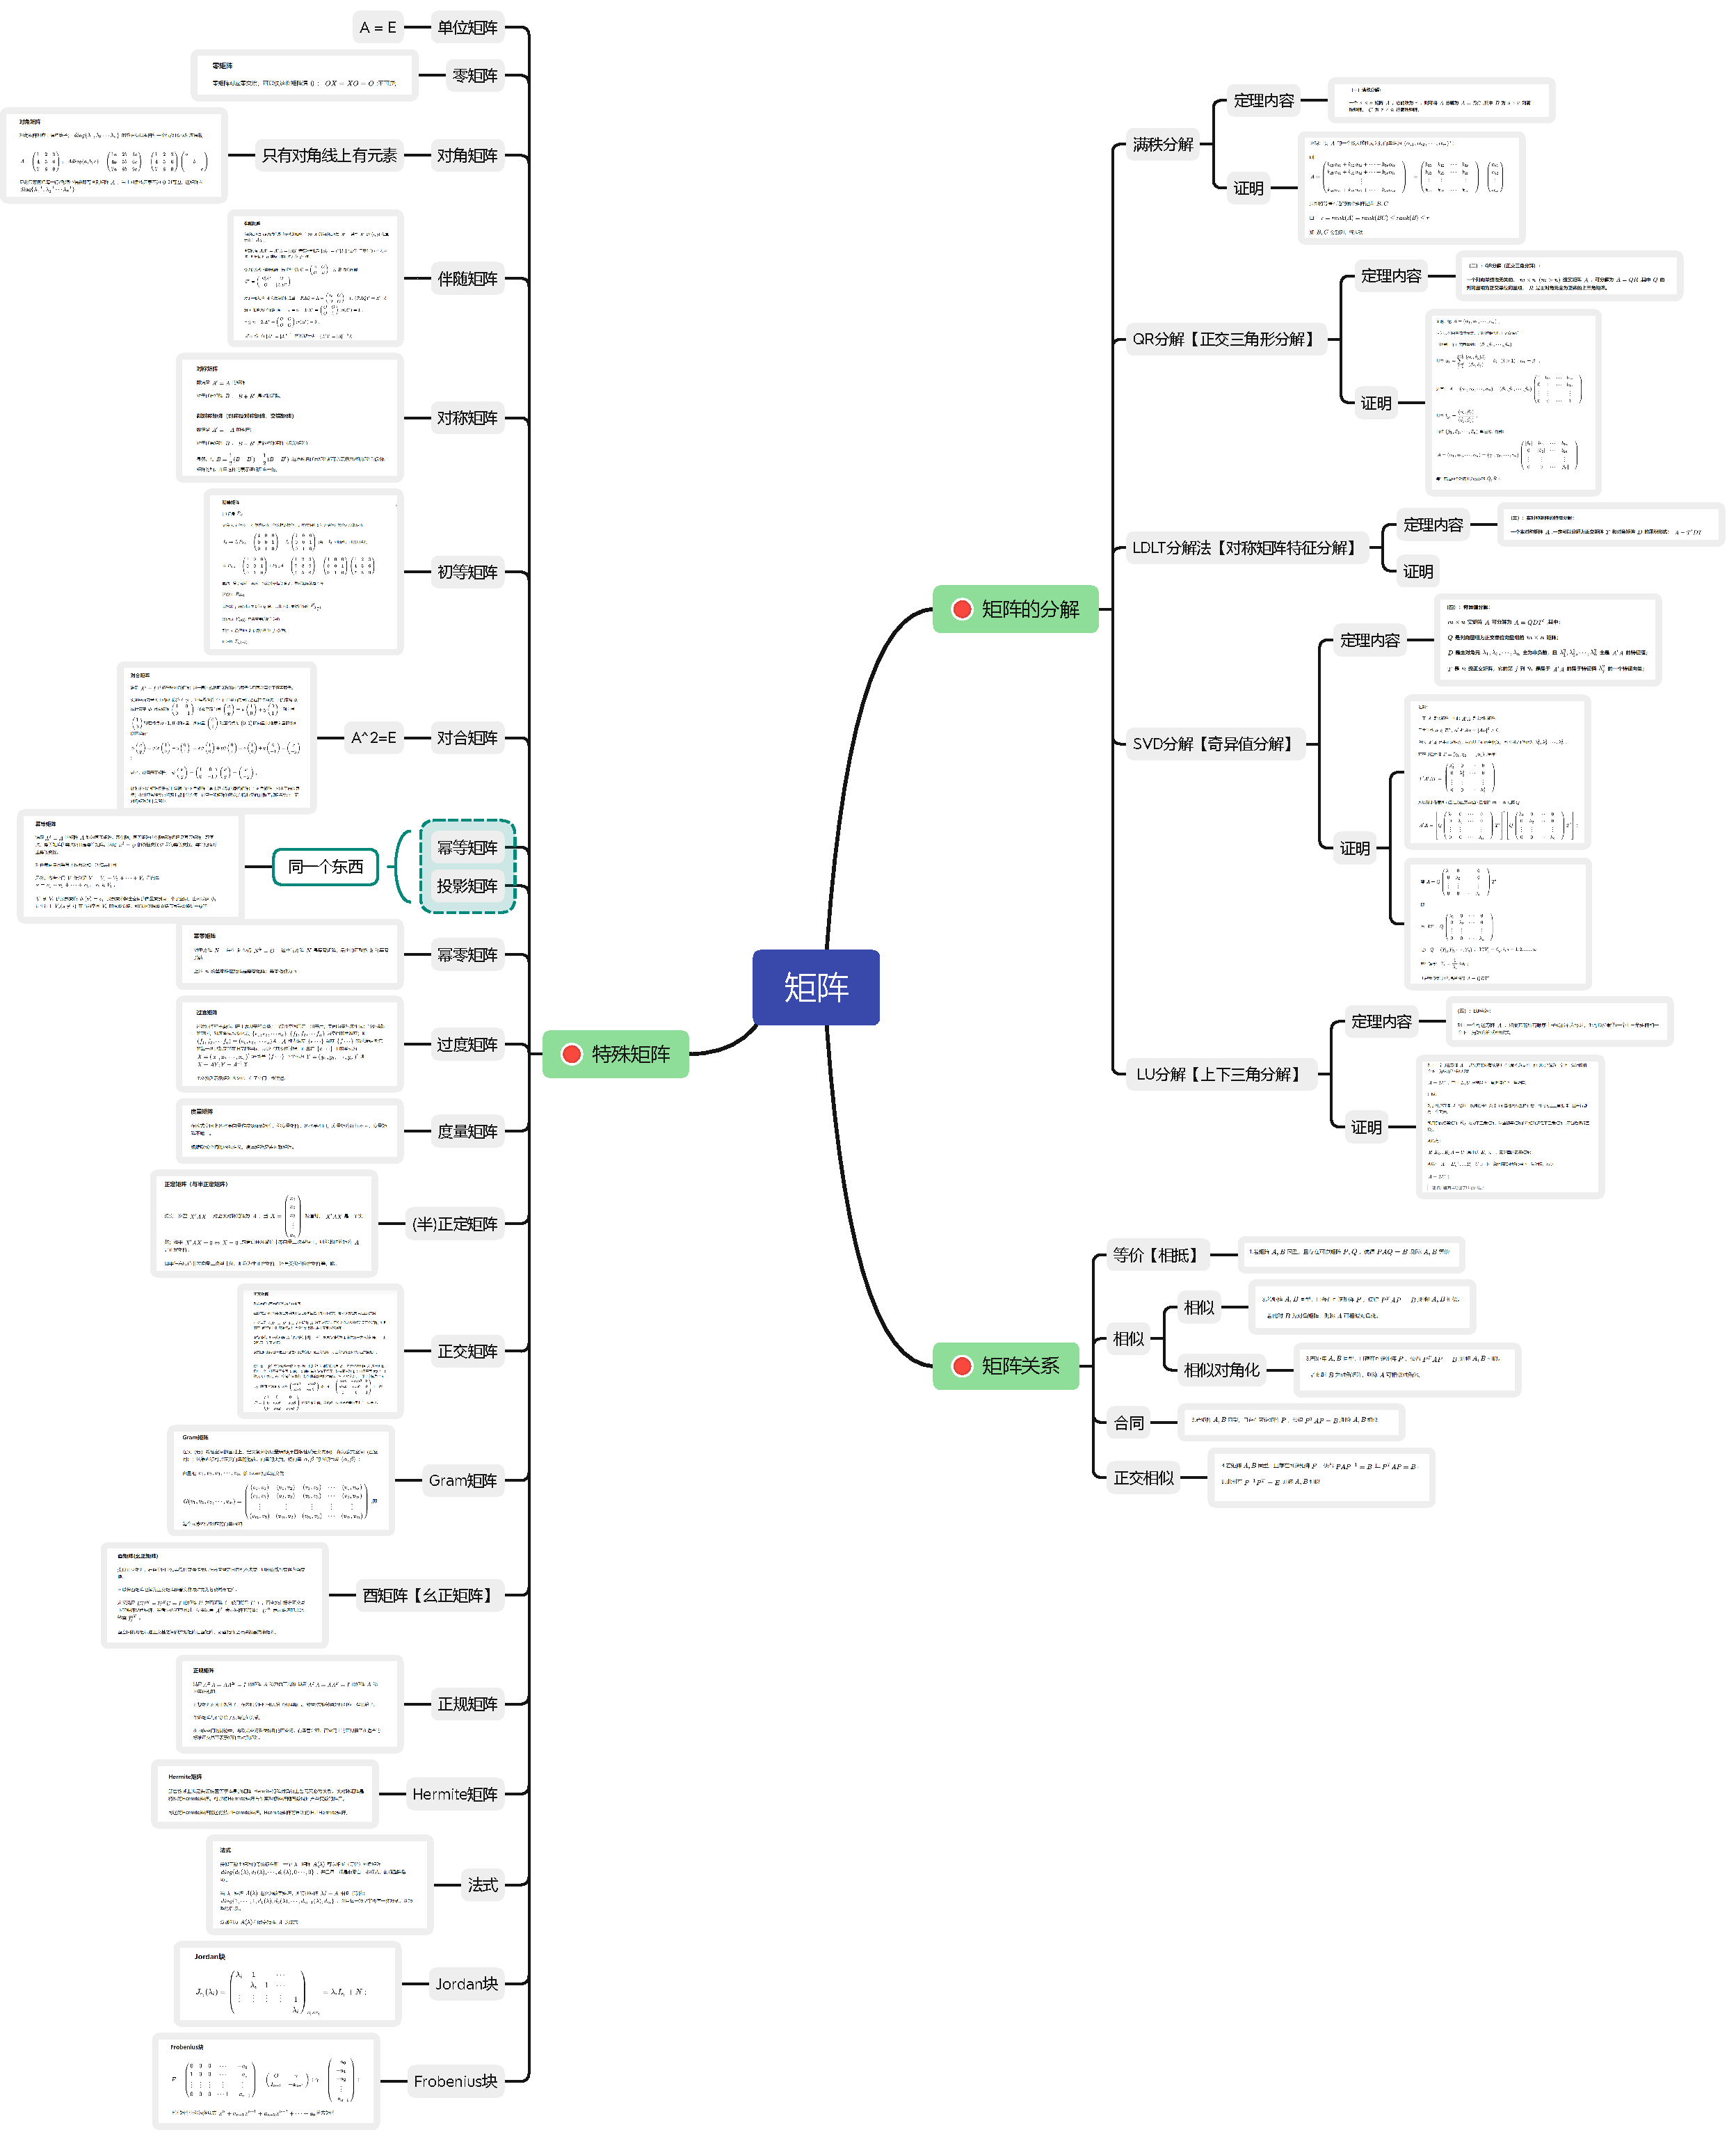
\includegraphics[scale=0.4]{Chapter/TikZ/矩阵.pdf}
    \label{矩阵}
    \caption{矩阵关系}
\end{figure}


\section{和式}
引入:看到一个双重求和的和式,但是我自己不会计算,很烦……
\begin{align*}
    \sum _{i=0}^n \left[\sum _{j=1}^{n-i} j^2\right]=\frac{1}{12} n (n+1)^2 (n+2)
\end{align*}

\textsf{轮换求和与对称求和}

两种形式
\[\sum_{cyc}^{}{}\hspace*{0.5\linewidth}\sum_{ sym}^{}{}\]

弄明白,尽量联系不等式里边的这两个东西。因为似乎在用了这个东西可以简化运算。

\subsection{轮换式中的根}
假如原来有一个根 $x =a$, 也就是说我们有$(x-a)(\cdots)= 0$。 
我们把$x\to y$, 可以得到$(y-a) (\cdots )=0$。 明显这个式子有一个根$y =a$。 
又因为这个式子是轮换的,所以可以得出后边的式子和前边的式子完全相同。
也就是说前边的式子一定有一个根$y =a$。 于是我们就可以知道原来的式子有两个根,
分别为$x = a, y=a$

\section*{求和符号基础知识}
\textsf{对称式:}三元任意换仍未原式

$x\Rightarrow y, y\Rightarrow z, z\Rightarrow x$.换完以后整体式子和原来恒等,比如$x+y+z, x^2 + y^2 + z^2, xy + yz + xz$ 

\textsf{对称式:}依序(正反序)互换后仍为原式
\newpage

\subsection{常见的和式恒等变换}
\begin{theorem}[和式恒等变换]
    \begin{align*}
    \num{1}\qquad & \left[\sum_{i=1}^{n}{a_i}\right]^2
        & = &\qquad\qquad \sum_{i=1}^{n}{a_i^2} + 2\sum_{1 \le i \le i \le n}{a_i a_j}\\
    % 
    % 
    \num{2}\qquad & \left[\sum_{1 \le i \le i \le n}{(a_i - a_j)}\right]^2
        & = &\qquad\qquad n\sum_{i=1}^{n}{a_i^2} - \left[\sum_{i=1}^{n}{a_i}\right]^2\\
    % 
    % 
    \num{3}\qquad & \left[\sum_{i=1}^{n}{a_i}\right] \left[\sum_{i=1}^{n}{b_i}\right]
        & = &\qquad\qquad \sum_{i=1}^{n}{\sum_{j=1}^{n}{a_i b_j}} = \sum_{j=1}^{n}{\sum_{i=1}^{n}{a_i b_j}}\\
    % 
    % 
    \num{4}\qquad & \left[\sum_{1 \le i \le i \le n}{a_ia_j}\right]^2
        & = &\qquad\qquad \sum_{i=1}^{n}{\sum_{j=1}^{n}{a_i a_j}} = \sum_{j=1}^{n}{\sum_{i=1}^{n}{a_i b_j}}\\
    % 
    %
    \num{5}\qquad & \sum_{i=1}^{n}{\sum_{j=1}^{n}{a_i a_j}}
        & = &\qquad\qquad \sum_{i=1}^{n}{a_i^2} + \frac{1}{2} \sum_{i=1}^{n}{\sum_{j=1}^{n}{[a_i b_j + a_j b_i]}}\\
    % 
    %
    \num{6}\qquad & \sum_{i=1}^{n-1}{\biggl(a_{i+1}-a_i\biggr)}
        & = &\qquad\qquad a_n-a_1\\
    % 
    %
    \num{7}\qquad & \sum_{i=1}^{n}{a_ib_i}
        & = &\qquad\qquad \sum_{i=1}^{n-1}{\bigg[(a_i-a_{i+1})B_i\bigg]} + a_nB_n\\
    % 
    %
    \num{8}\qquad & \sum_{i=m}^{n}{a_ib_i}
        & = &\qquad\qquad \sum_{i=m}^{n-1}{[(a_i-a_{i+1})B_i]} + a_nB_n - a_mB_{m-1}\\
    % 
    %
    \num{9}\qquad & \left[\sum_{i=1}^{n}{a_i^2}\right]\cdot \left[\sum_{i=1}^{n}{b_i^2}\right]
        & = &\qquad\qquad \left[\sum_{i=1}^{n}{a_ib_i}\right]^2 + \sum_{1\le i \le j \le n}({a_ib_j-a_jb_i})^2
    \end{align*}
\end{theorem}

\subsection{预备准备}
在证明之前,首先说明一个式子的几何意义,这对下面的证明有帮助
$\sum\limits_{1 \leq i<j \leq n} a_{i} a_{j} $,它的几何意义如下图,
其实就是一个 $(n-1)\times (n-1)$的上三角矩阵。

\begin{align*}
    \sum\limits_{1 \leq i<j \leq n} a_{i j}=
    \left|\begin{array}{cccc}
    a_{1} a_{2} & +a_{1} a_{3} & & +a_{1} a_{n} \\
    +a_{2} a_{3} & \cdots & +a_{2} a_{n} & \\
    \vdots & \ldots & & \\
    +a_{n-1} a_{n} & & & \\
    \end{array}\right|
\end{align*}


此外我们在这里引入另外一个记号$A$,具体的形式如下:
那么$A$旋转即可得到上边的$\sum\limits_{1 \leq i<j \leq n} a_{i j}$,其实$\sum\limits_{1 \leq i<j \leq n} a_{i j}$就是A的左下部分的旋转。

\begin{align*}
    {A}=\left|\begin{array}{ccccc}
    a_{1} a_{1} & & & \cdots & \\
    a_{2} a_{1} & a_{2} a_{2} & \cdots & & \\
    \cdots & \cdots & a_{3} a_{3} & & \\
    a_{n-1} a_{1} & \cdots & \cdots & \cdots & \\
    a_{n} a_{1} & a_{n} a_{2} & \cdots & a_{n} a_{n-1} & a_{n} a_{n}
    \end{array}\right|
\end{align*}



\subsection{等式的证明}
\begin{proof}\num{1}
    
\begin{align*}
    \left(\sum\limits_{i=1}^{n} a_{i}\right)^{2}
    & = \left(a_{1}+a_{2}+\cdots+a_{n-1}+a_{n}\right)^{2} \\
    & = a_{1}\left(a_{1}+a_{2}+\cdots+a_{n-1}+a_{n}\right)
    + a_{2}\left(a_{1}+a_{2}+\cdots+a_{n-1}+a_{n}\right) \\
    & \hspace*{16em}+ \cdots+a_{n}\left(a_{1}+a_{2}+\cdots+a_{n-1}+a_{n}\right) \\
    & = \left|
    \begin{array}{ccccc}
        a_{1} a_{1} & +a_{1} a_{2} & +a_{1} a_{3} & \cdots & +a_{1} a_{n} \\
        +a_{2} a_{1} & +a_{2} a_{2} & \cdots & & \\
        \cdots & \cdots & +a_{3} a_{3} & & \\
        +a_{n-1} a_{1} & \cdots & \cdots & \cdots & \\
        +a_{n} a_{1} & +a_{n} a_{2} & \cdots & +a_{n} a_{n-1} & +a_{n} a_{n}
    \end{array}
    \right|
     = \sum\limits_{\mathrm{i}=1}^{\mathrm{n}} a_{\mathrm{i}}^{2} + 2\sum\limits_{1 \leq i<j \leq n} a_{i} a_{j}\nonumber\\
    &\Longrightarrow \text{注:第i行即第i项}\nonumber
\end{align*}
\end{proof}


\begin{proof}\num{2}
\begin{align*}
    \sum_{1 \leq i<j \leq n}^{n}\left(a_{i}-a_{j}\right)^{2}
    & = \sum_{1 \leq i<j \leq n}^{n}\left(a_{i}^{2}-2 a_{i} a_{j}+a_{j}^{2}\right)\nonumber\\
    & = \left[\left(a_{1}^{2}-2 a_{1} a_{2}+a_{2}^{2}\right)+\cdots+\left(a_{1}^{2}-2 a_{1} a_{n}+a_{n}^{2}\right)\right] \\
    & + \left[\left(a_{2}{ }^{2}-2 a_{2} a_{3}+a_{3}^{2}\right)+\cdots+\left(a_{2}{ }^{2}-2 a_{2} a_{n}+a_{n}{ }^{2}\right)\right] 
      \quad + \left[\left(a_{n-1}^{2}-2 a_{n-1} a_{n}+a_{n}^{2}\right)\right]\\
    & = (n-1) \sum\limits_{i=1}^{n} a_{i}{ }^{2}-2\cdot
    \left|
    \begin{array}{cccc}
        a_{1} a_{2} & +a_{1} a_{3} & & +a_{1} a_{n} \\
        +a_{2} a_{3} & \cdots & +a_{2} a_{n} & \\
        \vdots & \ldots & & \\
        +a_{n-1} a_{n} & & & \\
    \end{array}
    \right|\\
    & =(n-1) \sum_{i=1}^{n} a_{i}{ }^{2}-2 \sum_{1 \leq i<j \leq n}^{n} a_{i} a_{j}\\
    & = n \sum_{i=1}^{n} a_{i}{ }^{2}-\left(\sum_{i=1}^{n} a_{i}{ }^{2}+2 \sum\limits_{1 \leq i<j \leq n}^{n} a_{i} a_{j}\right)
      = n \sum\limits_{i=1}^{n} a_{i}^{2}-\sum_{i=1}^{n} a_{i}^{2}
\end{align*}
\end{proof}


\begin{proof}\num{3}

\begin{align*}
    \left[\sum_{i=1}^{n} a_{i}\right]\times\left[\sum_{j=1}^{n} b_{j}\right]
    &=\left|
    \begin{array}{ccccc}
        a_{1} b_{1} & +a_{1} b_{2} & +a_{1} b_{3} & \cdots & +a_{1} b_{n} \\
        +a_{2} b_{1} & +a_{2} b_{2} & \cdots & \\
        \cdots & \cdots & +a_{3} b_{3} & & \\
        +a_{n-1} b_{1} & \ldots & \cdots & \cdots & \\
        +a_{n} b_{1} & +a_{n} b_{2} & \cdots & +a_{n} b_{n-1} & +a_{n} b_{n}
    \end{array}\right| \\
    &=a_{1} \sum_{j=1}^{n} b_{j}+a_{2} \sum_{j=1}^{n} b_{j}+\cdots+a_{n} \sum_{j=1}^{n} b_{j} \\
    &=\sum_{i=1}^{n}\left[a_{i}\left(\sum_{j=1}^{n} b_{j}\right)\right]
    =\sum_{i=1}^{n}\left[\left(\sum_{j=1}^{n} a_{i} b_{j}\right)\right] \\
    &=\sum_{i=1}^{n} \sum_{j=1}^{n} a_{i} b_{j}=\sum_{j=1}^{i \leftrightarrow j} \sum_{i=1}^{n} a_{j} b_{i} 
    =\sum_{j=1}^{n} \sum_{i=1}^{n} a_{i} b_{j}
    \Longrightarrow\text { 多重求和可以改变求和次序 }
\end{align*}
\end{proof}

\clearpage
\begin{proof}\num{4}

\begin{align*}
    \sum\limits_{1 \leq i<j \leq n} a_{i j}
    &=\left|
    \begin{array}{cccc}
        a_{1}a_{2} & +a_{1} a_{3} & & +a_{1} a_{n} \\
        +a_{2} a_{3} & \cdots & +a_{2} a_{n} & \\
        \vdots & \ldots & & \\
        +a_{n-1} a_{n} & & &\\
    \end{array}
    \right|\\
    &=a_{1}\sum_{j=1+1}^{n} a_{j}+a_{2} \sum_{j=2+1}^{n} a_{j}+\cdots+a_{n-1} \sum_{j=(n-1)+1}^{n} a_{j}
    \Longrightarrow\mbox{以前标为基准, i为前标} \\
    &=\sum_{i=1}^{n-1}\left[a_{i}\left(\sum_{j=i+1}^{n} a_{j}\right)\right] 
    =\sum_{i=1}^{n-1}\left[\sum_{j=i+1}^{n} a_{i} a_{j}\right]
    =\sum_{i=1}^{n-1} \sum_{j=i+1}^{n} a_{i} a_{j}\\
    & \Longrightarrow\mbox{以}45^{\circ}\mbox{线为轴:以斜标为基准, j为前标}\\
    & = \left(a_{1}\right) a_{2}+\left(a_{1}+a_{2}\right) a_{3}+\cdots+\left(a_{1}+a_{2}+\cdots+a_{n-1}\right) a_{n}\\
    & = a_{2} \sum_{j=1}^{2-1} a_{j}+a_{3} \sum_{j=1}^{3-1} a_{j}+\cdots+a_{n}\sum_{j=1}^{n-1} a_{j}\\
    & =\sum_{i=2}^{n}\left[a_{i}\left(\sum_{j=1}^{i-1} a_{j}\right)\right]
    =\sum_{i=2}^{n}\left[\left(\sum_{j=1}^{i-1} a_{i} a_{j}\right)\right] \\
    & =\sum_{i=2}^{n} \sum_{j=1}^{i-1} a_{i} a_{j} \Longrightarrow  \mbox{注:先取定外面的i值再展开内层}\\
\end{align*}

若以后标为基准将方阵变化一下即有:
\begin{align*}
 LHS&=\left|
    \begin{array}{ccccc}
        +a_{1} a_{2} & +a_{2} a_{3} & +a_{3} a_{4} & \cdots & a_{n-1} a_{n} \\
        +a_{1} a_{3} & +a_{2} a_{4} & \vdots & \cdots& \\
        +a_{1} a_{4} & \vdots & +a_{3} a_{n} & & \\
        \vdots & +a_{2} a_{n} & & & \\
        +a_{1} a_{n} & & &
    \end{array}
    \right|
\end{align*}
由对偶性知($i, j$只是一个记号而已), 
\[
    LHS=\sum_{j=1}^{n-1}\sum_{i=j+1}^{n}a_{i}a_{j}    
\]
\end{proof}



\begin{proof}\num{5}
\begin{align}
\sum_{i=1}^{n}{\sum_{j=1}^{n}{a_i a_j}}
&=\frac{1}{2}\left(\sum_{{i}=1}^{{n}} \sum_{{j}=1}^{{n}} a_{{i}} {b}_{{j}}+\sum_{{i}=1}^{{n}} \sum_{{j}=1}^{{n}} a_{{i}} {b}_{{j}}\right) \nonumber\\
&=\frac{1}{2} \sum_{{i}=1}^{{n}} \sum_{{j}=1}^{{n}}\biggl[a_{{i}} {b}_{{j}}+a_{{j}} {b}_{{i}}\biggr]\nonumber
\end{align}
\end{proof}

\begin{proof}\num{6}
\begin{align*}
    \sum_{i=1}^{n-1}\left(a_{i+1}-a_{i}\right)
    &=\left(a_{2}-a_{1}\right)+\left(a_{3}-a_{2}\right)+\ldots+\left(a_{n}-a_{n-1}\right) \\
    &=\left(a_{n}-a_{n-1}\right)+\ldots+\left(a_{3}-a_{2}\right)+\left(a_{2}-a_{1}\right) \\
    &=a_{n}-a_{1}
    \Longrightarrow\mbox{此式即为伸缩求和}
\end{align*}
\end{proof}
\clearpage


\begin{proof}\num{7, 8}

证法一

首先把所有的 $\mathrm{i}\rightarrow \mathrm{i}+1 $, 于是有 $n\to n-1$. 证法一(图解法),见陈纪修课本
\begin{align*}
    \sum_{i=2}^{n} A_{i-1} b_{i}=\sum_{i=1}^{n-1} A_{i} b_{i+1}
\end{align*}


证法二

\begin{align*}
    \sum_{i=m}^{n} a_{i} b_{i} 
    &=\sum_{i=m}^{n}\left[\left(A_{i}-A_{i-1}\right) b_{i}\right]
        = \sum_{i=m}^{n} A_{i} b_{i}-\sum_{i=m}^{n} A_{i-1} b_{i} \\
    &=\left(\sum_{i=m}^{n-1} A_{i} b_{i}+A_{n} b_{n}\right)-\sum_{i=m-1}^{n-1} A_{i} b_{i+1}
        \Longrightarrow\text { 把 } A_{i-1} \text { 变为 } A_{i} \text {, 方便后边提取公因式 } \\
    &=\sum_{i=m}^{n-1} A_{i} b_{i}+A_{n} b_{n}-\left[\sum_{i=m}^{n-1} A_{i} b_{i+1}+A_{\mathrm{m}-1} b_{m}\right]
        \Longrightarrow\text { 把求和范围变为相同 } \\
    & =\sum_{i=m}^{n-1}\left(A_{i} b_{i}-A_{i} b_{i+1}\right)+A_{n} b_{n}-A_{m-1} b_{m}
        =\sum_{i=m}^{n-1} A_{i}\left(b_{i}-b_{i+1}\right)+A_{n} b_{n}-A_{m-1} b_{m}\\
    &\mbox{注: 此式即为Abel分部求和}
\end{align*}

 
证法三

\begin{align*}
    \sum_{i=1}^n a_i b_i
    &=a_1 b_1+a_2 b_2+a_3 b_3+\cdots+a_n b_n \\
    &=b_1\left(A_1-A_0\right)+b_2\left(A_2-A_1\right)
        +b_3\left(A_3-A_2\right)+\cdots+b_n\left(A_{n-1}-A_n\right) \\
    &=\left(b_1-b_2\right) A_1+\left(b_2-b_3\right) A_2+\left(b_4-b_3\right) A_3
        +\cdots+\left(b_{n-1}-b_n\right) A_{n-1}+b_n A_n-b_1 A_0 \\
    &=\sum_{i=1}^{n-1} A_i\left(b_i-b_{i+1}\right)+b_n A_n
\end{align*}
\end{proof}


\begin{theorem}[Abel分部求和]
    \begin{align}
        \sum_{i=m}^{n}{a_ib_i}=\sum_{i=m}^{n-1} A_{i}\left(b_{i}-b_{i+1}\right)+A_{n} b_{n}-A_{m-1} b_{m}
    \end{align}
\end{theorem}

\textsf{关于Abel分部求和公式的几点讨论}

\ensuremath{\langle 1 \rangle} 若定义 $A_0=0$ ,那么当 $m=1$ 时即有
\[
    \sum_{i=1}^n a_i b_i 
    = \sum_{i=1}^{n-1} A_i\left(b_i-b_{i+1}\right)+A_n b_n
\]

\ensuremath{\langle 2 \rangle} 若 $a_i$ 不便于求和,那么便有如下的Abel和差变换
\[
    \sum_{i=m}^n\left(A_i-A_{i-1}\right) b_i 
    = \sum_{i=m}^{n-1} A_i\left(b_i-b_{i+1}\right)+A_n b_n-A_{\mathrm{m}-1} b_m
\]

\clearpage

\begin{proof}\num{9}
    \begin{align*}
    &\left(\sum_{i=1}^n a_i^2\right)\left(\sum_{i=1}^n b_i^2\right)-\sum_{i=1}^n\left(a_i b_i\right)^2
        = \sum_{i=1}^n \sum_{j=1}^n a_i^2 b_j^2-\sum_{i=1}^n \sum_{j=1}^n a_i b_i a_j b_j \\
    & = \frac{1}{2} \sum_{i=1}^n \sum_{j=1}^n\left(a_i{ }^2 b_j^2-2 a_i b_i a_j b_j+a_j{ }^2 b_i{ }^2\right)
        =\frac{1}{2} \sum_{i=1}^n \sum_{j=1}^n\left(a_i b_j-a_j b_i\right)^2 \\
    & = \sum_{1 \leq i<j \leq n}\left(a_i b_j-a_j b_i\right)^2
    \end{align*}
    注:柯西不等式即证毕
\end{proof}

\begin{theorem}[拉格朗日恒等式]
    \begin{align}
        \left[
        \sum_{i=1}^{n}{a_i^2}
        \right]
        \cdot 
        \left[
        \sum_{i=1}^{n}{b_i^2}
        \right]
        &=
        \left[
        \sum_{i=1}^{n}{a_ib_i}
        \right]^2
        +
        \sum_{1\le i \le j \le n}({a_ib_j-a_jb_i})^2
    \end{align}
\end{theorem} 
    -\section{同构线性空间性质}

\subsection{同构的理解}
若$\alpha = \beta + \gamma$, 则$\sigma(\alpha + \beta) = \sigma(\gamma) = \sigma(\alpha) + \sigma(\beta)$

\begin{figure}[!htb]
    \centering
    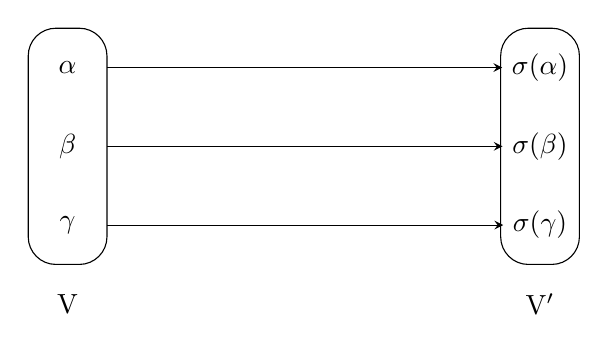
\begin{tikzpicture}[>=stealth]
        \draw[rounded corners=1em] (0, 0.5) rectangle (1, 3.5);
        \draw[rounded corners=1em] (6, 0.5) rectangle (7, 3.5);
        \node (A1) at (.5, 3) {$\alpha$};
        \node (B1) at (.5, 2) {$\beta$};
        \node (C1) at (.5, 1) {$\gamma$};
        \node (A2) at (6.5, 3) {$\sigma(\alpha)$};
        \node (B2) at (6.5, 2) {$\sigma(\beta)$};
        \node (C2) at (6.5, 1) {$\sigma(\gamma)$};
        \node at (.5, 0) {${\rm V}$};
        \node at (6.5, 0) {${\rm V'}$};
        \draw[->] (A1)++(.5, 0)--(A2);
        \draw[->] (B1)++(.5, 0)--(B2);
        \draw[->] (C1)++(.5, 0)--(C2);
    \end{tikzpicture}
    \caption{映射关系图}
    \label{映射关系图}
\end{figure}

% \begin{figure}[!htb]
%    如下图所示:
%         \ctikzfig{Chapter/TikZ/Visaul_Mapping}
%         \caption{映射关系图}
% \end{figure}

\noindent\num{1}\quad  $\alpha+\beta=\gamma \Rightarrow \sigma(\alpha)+\sigma(\beta)=\sigma(\gamma)$.
前面相等决定了后面一定相等\\
\num{2}\quad 因为是双射,所以我们也可以认为是$V'$中的每个元素都会被$V$中的元素所决\\ 
\num{3}\quad 我们把映射$\sigma$取逆,则可知:$V$中的每个元素被$V'$中的两个元素确定\\ 
\num{4}\quad 从2, 3点我们可以知道:$V$与$V'$中的对应元素的关系相同\\    

\begin{corollary}[线性空间的结构]
   所以我们可以认为线性空间的结构就是:\\ 
   \num{1} 元素的个数\\ 
   \num{2} 元素之间的关系(我们定义的加法和数乘)
   
   综上:

$\sigma(\sigma^{-1})$的存在,使得$V(V')$中的元素均被$V'(V)$中的元素确定。确定了数乘与加法以及相同的元素个数,所以$\sigma (\sigma^{-1})$使得$V$与$V'$有了不同的结构。           
\end{corollary}


\clearpage
\subsection{同构的线性空间具有相同的维数的证明}
\begin{proof}{\bf 错误的证明}\par
    如图\ref{映射关系图}所示:$\sigma: \alpha_i - \beta_i, ~\alpha_i \in V, \beta_i \in V'$
    是一个线性同构映射(只能够 $1-1$对应),那么我们就有
    \begin{align*}
        &\sigma(\alpha+\beta) = \sigma(\alpha) +\sigma(\beta)\\
        & \sigma(k\alpha) = k \sigma(\alpha)
    \end{align*}
    假如两个向量空间
    中的基向量的个数不相同,那么肯定不能够实现 $1-1$对应,所以矛盾。

    \bigskip
    ~~若 $V$的基为 \{\seq{\alpha}\}, $V$中的向量 \{\seq[s]{\beta}\} (不一定是基)。
    令 $\sigma(\alpha_i) = \sigma(\beta_i)$, 其中 $s>n$,则有
    \begin{align*}
        k_1\alpha_1 + \cdots + k_n\alpha_n = 0, \mathtext{其中} k_i = 0
    \end{align*}
    那么一定有
    \begin{align*}
     & \sigma(k_1\alpha_1 + \cdots + k_n\alpha_n)
        \rightarrow\mathtext{根据法则1:因为} k_i\alpha_i \in V\\ 
    =& \sigma(k_1\alpha_1) + \sigma(k_2\alpha_2 + \cdots + k_n\alpha_n)
        = \sigma(k_1\alpha_1) + \sigma(k_2\alpha_2) + \sigma(k_3\alpha_3 + \cdots + k_n\alpha_n)\\
    ~&\vdots\\
    =& \sigma(k_1\alpha_1) + \sigma(k_2\alpha_2) + \cdots + \sigma(k_n\alpha_n)
        \rightarrow \mathtext{根据法则2:} k_i\alpha_i \in V'\\
    =&  k_1\sigma(\alpha_1) + k_2\sigma(\alpha_2) + \cdots + k_n\sigma(\alpha_n)
        = k_1 \beta_1 + \cdots + k_n\beta_n\\
    =& 0
    \end{align*} 
    又因为 
    \[
    \displaystyle \sum_{i=1}^{n}{k_i\alpha_i}  = \sigma(\theta) = \theta
    = \sigma(\sum_{i=1}^{n}{k_i\alpha_i})
    = \sum_{j=1}^{n}{k_j\beta_j}
    = \theta\Rightarrow k_i = 0
    \]
    所以就可以得出 $\dim(\beta) \ge n$

    若 $\dim(\beta) \ge n$ 令 \seq[s]{\beta}, ~~(s>n),
    由于 $\sigma$ 是双射, 所以存在逆映射 $\sigma^{-1}$,
    使得
    \[
        \sigma^{-1}(\beta) = \alpha    
    \]
    同理,仿照上面的证明过程我们可以得到
    \[
        \dim(\alpha) \ge n
    \] 
    因为 $\beta_i, ~~i\in \{1, 2, \cdots, s\}$线性无关,则:
    \im{\sum_{i=1}^{s}{k_i\beta_i}}中 $k_i=0 \Rightarrow$ 
    \im{\sigma(\sum_{i=1}^{s}{k_i\beta_i})=\theta}, 
    即 
    \[
    \im{\sum_{i=1}^{s}{k_i\sigma(\beta_i)} = \sum_{i=1}^{s}{k_i\alpha_i} = \theta}
    \]
    那么就可以得到 $\dim(\alpha)>n$, 然而这与 $\dim(\alpha)=n$矛盾。
    于是可以得证:同构的线性空间具有相同的维数
\end{proof}

\begin{proof}{\bf 正确的证明}

    构造映射 $\sigma: \alpha_i - \beta_i, ~\alpha_i \in V, \beta_i \in V'$
    是一个线性同构映射(只能够 $1-1$对应),那么我们就有如下的两条性质:
    \begin{align*}
        &\sigma(\alpha+\beta) = \sigma(\alpha) +\sigma(\beta) \tag{1}\\
        & \sigma(k\alpha) = k \sigma(\alpha) \tag{2}
    \end{align*}

    \bigskip
    ~~若 向量空间$V$的基向量为 \{\seq{\alpha}\}, 向量空间$V'$中的向量 \{\seq[s]{\beta}\} (不一定是基)。
    构造一个向量。注:以下均假设 $\theta$是一个零元素(零向量):
    \[ 
    \im{\alpha = \sum_{i=1}^{n}{k_i\alpha_i} = \theta}
    \]
    因为 $\alpha_i$是 $V$的基。 所以$k_i=0$是上述方程的唯一解,于是有:

    \begin{minipage}[c]{0.3\linewidth}
        \vspace*{0pt}
        \begin{align*}
            \sigma(\sum_{i=1}^{s}{k_i\alpha_i})
            &\xlongequal[]{\mbox{\tiny 性质(1)}}  \sum_{i=1}^{s}{\sigma(k_i\alpha_i)}\\
            & \xlongequal[]{\mbox{\tiny 性质(2)}}  \sum_{i=1}^{s}{k_i\sigma(\alpha_i)}\\ 
            & =  \sum_{i=1}^{s}{k_i \beta_i} = \sum_{i=1}^{s}{\sigma(\alpha)} \\
            & =  \sum_{i=1}^{s}{\sigma(\theta)} = \theta\\
        \end{align*}
    \end{minipage}
        \hfill
    \begin{minipage}[c]{0.65\linewidth}
        \vspace*{0pt}
        \begin{formal}{blue!20}
            在这里说明,若 $\exists k_i \neq 0$, 则有矛盾;
            因为 $\sigma$是双射, 故存在唯一的逆映射 $\sigma^{-1}$,使得:\\
            \hspace*{3em}\im{\sigma^{-1}:~ \beta_i \rightarrow \alpha_i, ~ \beta_i \in V', \alpha_i \in V}  \\
            同样满足方程(1)(2),于是就有:\\
            \hspace*{1em}\im{
                \sigma^{-1} (\sum_{i=1}^{s}{k_i\beta_i}) 
                 = \sum_{i=1}^{s}{k_i\sigma^{-1}(\beta_i)}
                 = \sum_{i=1}^{s}{k_i\alpha_i} = \theta
            }\\
            若存在 $k_i\neq 0$, 那么就与前面的 $k_i=0$ 矛盾。 
        \end{formal}
    \end{minipage}

    \bigskip
    故 $\beta_i$ 线性无关。所以可以知道:$\dim(V')\ge n$, 下面证明若 $\dim(\beta)> n$则矛盾,若推出了矛盾,
    也就证明了 $\dim{V'} = n = \dim{V}$。不妨设 \seq[s]{\beta}为 $V'$的基,则
    \begin{align*}
        \sigma(\sum_{i=1}^{s}{l_i\beta_i}) = \sum_{i=1}^{s}{l_i\sigma(\beta_i)} = \sum_{i=1}^{s}{l_i\alpha_i}
    \end{align*}
    令 \im{\beta = \sum_{i=1}^{s}{l_i\beta_i} = \theta} , 则根据前面的证明过程可以知道 $l_i=0$,是此方程的唯一解。
    又因为解的唯一性,并且有 \im{\sigma(\theta) = \theta = \sum_{i=1}^{s}{l_i\alpha_i}},故 $l_i=0$是唯一解.
    所以可以得出 $V$的基向量个数为 $s(>n)$, 但是这与 $\dim(V)=n$ 矛盾。\textsf{证毕} $\square$
\end{proof}

\subsection{一个思考}
\begin{formal}{blue!20}
    \textsf{思考一:同解问题}\par 
    \ttfamily
    其实我认为这里有一个 $\sigma$映射下的同解性问题. 即:若方程
    \[
        \sum_{i=1}^{s}{k_i\alpha_i} = 0 \tag{*}
    \]
    有解 $\vec{K} = \{k_1, \cdots, k_s\}$
    我在上述方程的两边同时做映射 $\sigma$,那么可以得到 
    \[
        \sigma(\sum_{i=1}^{s}{k_i\alpha_i}) = \sigma(\theta) = \theta     \tag{**}
    \]

    于是可以知道方程 (**)的解为方程(*)的解。
    也就是说方程 (*)和方程 (**)同解, 即 $\sigma$ 作用下方程同解。
    因为 映射 $\sigma$ 只有
    作用于 零元素才可以得到零元素(向量空间的性质).
    \begin{center}
        若 $\sigma$是线性同构映射~$\Rightarrow \sigma(\alpha)= \beta$的$\alpha$是唯一的
    \end{center}
\end{formal} 


\begin{formal}{blue!20}
    \textbf{思考二:线性同构与线性变换的区别}\par 
    在线性变换中我们有:若 $\mathscr{A}$为一个线性变换,
    令 $k_1\alpha_1 + \cdots + k_n\alpha_n = \theta$,则我们可以得到:
    \[
        \mathscr{A}(k_1\alpha_1 + \cdots + k_n\alpha_n) = k_1\mathscr{A}(\alpha_1) + \cdots + k_n\mathscr{A}(\alpha_n) = \theta   
    \] 
    这里的变换 $\mathscr{A}$不是 $1-1$映射,其实就是使得 $\mathscr{A}(\gamma)=\theta$的 $\gamma$不是唯一的。

    结合上边的例子来解释就是:
    \[
        \mathscr{A}\im{\left(\sum_{i=1}^{s}{k_i\alpha_i}\right) = \theta \nRightarrow \sum_{i=1}^{s}{k_i\alpha_i}=\theta} 
    \]
    也就是说若 $\vec{K_0} = \{k_1, \cdots, k_s\}$是方程 \im{\sum_{i=1}^{s}{k_i\alpha_i}}的解,我们可以得到:
    \[
        \sum_{i=1}^{s}{k_i\alpha_i} = \mathscr{A}(\theta) = \theta
    \]
    但是如果我们有:
    \[
        \mathscr{A}\im{\left(\sum_{i=1}^{s}{k_i\alpha_i}\right)} = \theta
    \]
    那么此时 $K_0$肯定是这个方程的 \textbf{一个}解,但是这个方程很可能还有其他的非零元解
    (因为变换 $\mathscr{A}$不一定可逆, 它可以把一个非零向量 ${\sum\limits_{i=1}^{s}{k'_i\alpha_i}=\theta,~k'\neq k}$映射为一个零元素)。
    我们把这个解记为 $K'$, 那么明显 $K'\neq K_0$。也就是说此时满足:
    \im{
        \mathscr{A}\im{\left(\sum_{i=1}^{s}{k_i\alpha_i}\right)} = \theta
    }
    的解 $K'$, 不能够满足方程\im{\sum_{i=1}^{s}{k_i\alpha_i}=\theta}
\end{formal}

\clearpage
    \section{子空间为直和的几个等价条件}

\subsection{证明思路}
首先说明直和的几个等价条件:

\begin{framed}
\noindent
\num{1} 定义:$V_1\oplus V_2$\\
\num{2} 零向量 $\theta$ 的分解唯一\\
\num{3} $V_1\bigcap V_2=\theta$\\
\num{4} $\dim(V_1+V_2)=\dim(V_1)+\dim(V_2)$\\
\num{5} 若\seq[n_1]{\alpha}和\seq[n_2]{\beta}分别为向量空间$V_1,V_2$的一组基,
        那么\seq[n_1]{\alpha}~,~\seq[n_2]{\beta}是 $V_1+V_2$的一组基
\end{framed} 

\bigskip
我们只需要证明:$1 \Rightarrow 2 \Rightarrow 3 \Rightarrow 4 \Rightarrow 5 \Rightarrow 1$即可
(注:$\Rightarrow $表示能够推出)

\begin{proof}{${1} \Rightarrow  {2}$}

   当 $V_1\oplus V_2$时, $\theta = \alpha_1 +\alpha_2, ~~\alpha_1 \in V_1,\alpha_2\in V_2$的分解唯一\par 
   又因为 $\alpha_1 = \alpha_2=\theta$是上述方程的一个解。\par 
   因为解的唯一性,我们可以知道 $\alpha_1=\alpha_2=\theta$\par
   于是我们可以得到: $\theta =\alpha_1+\alpha_2$,当且仅当 $\alpha_1=\alpha_2=\theta$时成立\par
   证毕 $\square$
\end{proof}

\begin{proof}{${2} \Rightarrow {3}$}

    $\forall \alpha \in V_1\bigcap V_2$, 因为 $V_1\bigcap V_2$为一个子空间, 所以 $-\alpha\in V_1\bigcap V_2$\par 
    又因为子空间的封闭性,所以我们有 $\alpha+(-\alpha)=\theta\in V_1\bigcap V_2$.\par 
    根据上面 ${1} \Rightarrow {2}$的证明我们可以知道:$\alpha =-\alpha=\theta$\par
    最后根据 $\alpha$的任意性,可以知道 $v_1 \bigcap V_2=\theta$\par 
    证毕 $\square$
\end{proof}

\bigskip
\begin{proof}{${3} \Rightarrow {4}$}

    根据维数公式,我们可以得到: $\dim(V_1+V_2) =\dim(V_1) + \dim(V_2) -\dim(V_1\bigcap V_2)$.
    对于任意的 $\alpha\in V_1 \bigcap V_2$, 必然有 $\alpha =\theta$.(因为两个向量空间 $V_1, V_2$ 的交集为空集).
    故此结论显然\par 
    证毕 $\square$
\end{proof}

\bigskip
\begin{proof}{ ${4} \Rightarrow {5}$ }

    设\seq{\alpha},~\seq{\beta}分别为 $V_1, V_2$的基。根据子空间和的定义我们有:
    \[
        \seq[n_1]{\alpha},~\seq[n_2]{\beta}
    \]
    是 $V_1 +V_2$的一组基.设 $\forall \alpha\in V_1 +V_2$, 则:
    \[
        \alpha = \underbrace{\sum_{i=1}^{n_1}{k_i\alpha_i}}_{\in V_1} + \underbrace{\sum_{i=1}^{n_2}{l_i\beta_i}}_{\in V_2}  =\theta   
    \]
    根据 ${3} \Rightarrow {4}$的结论,我们可以知道:
    \[
        \sum_{i=1}^{n_1}{k_i\alpha_i} = \sum_{i=1}^{n_2}{l_i\beta_i}  =\theta
    \]
    同时,又因为 \seq[n_1]{\alpha}, \seq[n_2]{\beta}是向量空间 $V_1, V_2$的基,所以可以得到:
    \[
        k_i= l_i=0,~i \in \{1, 2, \cdots\}
    \]
    同时又因为 \im{\mathbf{span}(\alpha_i) + \mathbf{span}{(\beta_i)} = V_1 + V_2},且 $\alpha_1, ~\beta_i$线性无关,所以可以得到结论\par 
    证毕 $\square$
\end{proof}

\begin{proof}{${5} \Rightarrow {1}$}

    设 $\forall \alpha  = \beta_i +\gamma_i \in V_1 + V_2,~ \beta_i\in V_1, \gamma_i \in V_2$.同时假设
    \begin{align*}
        \alpha =  \beta_1 + \gamma_1\\
        \alpha = \beta_2 + \gamma_2        
    \end{align*}

    因为 $\alpha =\theta$, 所以可以得到:
    \[
        (\gamma_1-\gamma_2) +  (\beta_1 -\beta_2) = \theta    
    \]
    根据上面 ${1} \Rightarrow {2}$的结论可以知道:
    \begin{align*}
        \beta_1 = \beta_2\\
        \gamma_1 = \gamma_2    
    \end{align*}
    于是乎,$\alpha$的分解就是唯一的\par 
    证毕 $\square$
\end{proof}


\begin{formal}{blue!20}
  {\bf 备注: }我们在证明的过程中多次用到 ${1} \Rightarrow {2}$的结论,但是这个并没有逻辑问题. 
\end{formal}
    

    \chapter{Ordinary Partial Equation}
    \newcommand{\coef}{\ensuremath{\displaystyle \mathrm{Exp}\{{-\int_{}^{}{p(x){\rm d}x}}\}}}
\newcommand{\ee}{\ensuremath{\mathrm{e}}}

\section{一阶线性微分方程的通解}
\begin{theorem}[一阶线性微分方程的通解]
     \begin{align}
          \mbox{标准形式:}\quad \frac{\dd y}{\dd x} + p(x)=q(x)&\nonumber\\
          &\mbox{通解:}\quad y=\mathrm{Exp}\{{-\int_{}^{}{p(x){\rm d}x}}\}\cdot\int_{}^{}{\biggl(\mathrm{Exp}\{{\int_{}^{}{p(x) {d\rm }x}}\} \cdot q(x)+C\biggr) {\rm d}x}
    \end{align}
\end{theorem}

\begin{proof}

首先两边同时乘以积分因子 \coef 即有:
\begin{align*}
     & \coef \cdot\frac{\dd y}{\dd x} + \coef \cdot p(x) = q(x)\cdot \coef \\
     \Longrightarrow\quad  & \frac{\dd }{\dd x}\biggl(y\cdot \coef \biggr)=q(x)\cdot\coef \\
     \Longrightarrow\quad  & y=\coef \cdot\int_{}^{}{\biggl(\coef \cdot q(x)\biggr)\dd x}
\end{align*}

下边说明第一个积分 
\[
    \coef = \gamma(x)
\]

不用加任意常数$C$, 假设
\[
    \coef = \gamma(x) + C    
\]

带入上边的式子即有
\begin{align*}
     y & =\quad  \ee^{-\gamma(x)-C}\cdot \int_{}^{}{e^{\gamma(x)+C}\cdot q(x) \dd x}\\
     & \Longrightarrow\quad  y=e^{-C}\cdot e^{-\gamma(x)}\cdot e^C\cdot \int_{}^{}{e^{\gamma(x)}\cdot q(x)\dd x}\\
     & \Longrightarrow\quad  y=e^{-\gamma(x)}\cdot\int_{}^{}{e^{\gamma(x)}\cdot q(x)\dd x}
 \end{align*} 

所以从上边我们可以看出,第一个积分可以不加常数C. 但是注意:上边只是非齐次方程的特解,
我们还应该加上齐次方程的通解,所以可以得到原微分方程的通解为:

\begin{framed}
    \begin{align*}
        y & = \ee^{-\int_{}^{}{p(x)\dd x}}\cdot\int_{}^{}{[\ee^{\int_{}^{}{p(x) \dd x}} \cdot q(x)+C] \dd x}
        = \mathrm{Exp}\{{-\int_{}^{}{p(x) \dd x}}\}\cdot\int_{}^{}{\biggl(\mathrm{Exp}\{{\int_{}^{}{p(x) {d\rm }x}}\} \cdot q(x)+C\biggr) \dd x}
    \end{align*}
\end{framed}
\end{proof}

\clearpage

\subsection{两个错误的带入公式的例子}
\begin{framed}
\[
    xy'+(x+1)y=\ee^x \hspace*{.5\linewidth} x'' -x = C_0   
\]
\end{framed}
\noindent{\bf 第一题}

{\bf 错解}

先求出齐次方程的通解
\[
    y={\rm Exp}\{\int_{}^{}{\frac{1+x}{x} dx}\}
\]
原来非齐次方程的解即为:
\begin{align*}
    y & = \ee^{\int_{}^{}{\frac{1+x}{x} \dd x}}[\int_{}^{}{e^{\int_{}^{}{\frac{1+x}{x} \dd x}}\cdot \frac{e^x}{x} \dd x}]
        = \ee^{\ln |x|+x}[\int_{}^{}{\ee^{\ln |x|+x} \cdot \frac{\ee^x} {x}\dd x}]\\
      & = |x|\ee^x\cdot\biggl(\int_{}^{}{\ee^{2x} \dd x}\biggr)
        = x\ee^x\cdot(\frac{1}{2}\ee^{2x}+C)
\end{align*}

\begin{formal}{blue!20}
    错因:积分因子乘过去没有取倒数
\end{formal}
{\bf 正解}

首先求得积分因子
\[
    \ee^{\int_{}^{}{\frac{x+1}{x} \dd x}}=x\ee^x    
\]
然后使用公式可以知道:
\begin{align*}
    & y = \frac{1}{x\ee^x}\cdot \int_{}^{}{\ee^x\cdot x\ee^x \dd x}
        = \frac{\ee^{-x}}{x}\cdot (\frac{1}{2}x\ee^x-\frac{1}{4}\ee^{2x}+C)
        = (\frac{1}{2}-\frac{1}{2x})\ee^x + C\cdot \frac{\ee^{-x}}{x}
\end{align*} 

仍然有错:原方程两边同时除以 $x$ 时没有对右边的 $e^x$ 除以 $x$.
只需要把第二种错误的解法稍微改善以下就可以得到正解
\begin{formal}{blue!20}
\[
    \displaystyle y = \frac{\ee^x}{2x}+C\cdot\frac{\ee^{-x}}{x}
\]
\end{formal}  

\noindent{\bf 第二题}

求解如下的二阶微分方程
\[
    x'' -x = C_0  \Longleftrightarrow x'' - x' + x' - x = 0
\]
即 $g'(t) - g'(t) = C_0$, 其中: $g(t) = x'(t) -x(t)$. 可以猜测 $g(t)$的形式如下:
\[
    g(t) = -C_0 + c\ee^{-t}    
\]
验证
\[
    g'(t) - g(t) = c\ee^{-t} -(-C_0 + c\ee^{-t}) = C_0    
\]
然后求解得到: $x'(t) - x(t) = c\ee^{-t} -C_0$.

但是如果直接代入公式是得不到正确 $g(t)$, 理由如下:
\begin{align*}
    g(t) = \ee^{-\int_{}^{}{-1}\dd t}\cdot \int_{}^{}{\ee^{\int_{}^{}{-1}}\dd t}
         = C_0 \ee^{t} (\ee^{-t}+\ee^{c_1}) 
         = C_0 + \ee^{c_1}\cdot C_0  e^t
         = C_0 + C\ee^t
\end{align*} 
    \newcommand{\dis}{\displaystyle}


\section{微分方程的常见解法}
已知有方程
\begin{framed}
    \begin{align*}
        (2x + \frac{1}{y}) \dd x  + (\frac{1}{y^2}-\frac{x}{y^2})\dd y = 0
    \end{align*}      
\end{framed}
    
\subsection{分项组合}
\[\frac{1}{y}\dd x -\frac{x}{y^2}\dd y=\dd\frac{x}{y}+x\dd\frac{1}{y}=2\cdot \dd\frac{x}{y}\] 

当时的错误想法:认为 $y$ 与 $x$ 无关,那么在 $\frac{1}{y}\dd x$ 中,$\frac{1}{y}$ 就是一个常数,常数当然可以拿到微分后边去。
所以后边$\dis \frac{x}{y^2}\dd y$当然也同理,认为 $x$ 与 $y$ 没有关系,于是就产生了这个错误。

\begin{formal}{blue!20}
    ~~认为 $x$ 与 $y$ 无关,它们都有一个微分方程的关系了,那么就可以认为 $y=y(x)$,必然二者有关系。也就是说 $x$ 不能随便的放到后边的 $\dd y$ 中了.
    
    今后$f(x)\dd x$可以把$f(x)$做一个积分,然后放到$\dd x$里边去, $f(y)\dd y$类似,但是遇到形如 $f(x)\dd y$ 或 $f(y)\dd x$的东西的时候
    一定要找前后的搭配
\end{formal}



\textsf{常见的凑微分形式}

\begin{corollary}[常见的凑微分形式]
\begin{align*}
    & x\dd y + y\dd x = \dd(xy)            \hspace*{22em}                          & & \frac{y\dd x-x\dd y}{y^2}=\dd(\frac{x}{y}) \\
    & \frac{y\dd x -xy}{x\dd y} = \dd\bigg[\ln(\frac{x}{y})\bigg]                  & & \frac{y\dd x-x\dd y}{x^2+y^2}=\dd\bigg[{\rm arccot}(\frac{y}{x})\bigg]\\
    & \frac{y\dd x-x\dd y}{x^2-y^2}=\frac{1}{2}\dd\bigg[\ln\biggl|\frac{x-y}{y-x}\biggr|\bigg] & & 
\end{align*} 
\end{corollary}

\subsection{曲线积分}
\noindent{\bf 错解}

因为已知有:$\dis u(x,y)=\int_{x_0}^{x}{M(x,y_0) \dd x}+\int_{y_0}^{y}{N(x,y) \dd y}$.
于是我们取点$(x_0,y_0)=(0, 1)$, 带入上边即有

\begin{align*}
u(x,y)& = \int_{0}^{x}{M(x,1) \dd x}+\int_{1}^{y}{N(x,y) \dd x}
        = \int_{0}^{x}{ 2x+1 \dd x}+\int_{1}^{y}{\bigg(\frac{1}{y}-\frac{x}{y^2}\bigg) \dd y}\\
      & = x^2 + x + C_1 + \ln|y|+\frac{x}{y} + C_2
\end{align*}
所以最终可以知道
\[
    u(x,y)=x^2+x+\ln|y|+\frac{x}{y}+C    
\]


\begin{formal}{blue!20}
    错因: 在$\dis \int_{1}^{y}{\bigg(\frac{1}{y}-\frac{x}{y^2}\bigg)}\dd y$中,当$y=1$时,有一个$\frac{1}{1}-\frac{x}{1}=1-x$, 但是我们忽略了它。
\end{formal}

\noindent{\bf 正解}

首先判断该方程是否为恰当微分方程,有$\dis \frac{\partial M}{\partial y}=\frac{-1}{y}=\frac{\partial N}{\partial x}$,所以该方程是一个恰当的微分方程。同时取点$(0, 1)$,于是就可以得到
\begin{align*}
    u(x,y) =\int_{0}^{x}{\frac{2xy+1}{y}\dd x + \int_{1}^{y}{\frac{y-0}{y^2}} \dd y} 
        = x^2+\frac{x}{y}+\ln|y|\bigg|_{1}^{y}
        = x^2+\frac{x}{y}+\ln|y|+C
\end{align*} 

\textsf{曲线积分方法}

\begin{theorem}[曲线积分法]
$
    \begin{aligned}
        \text{标准形式:}M(x,y)\dd x+N(x,y)\dd y=\frac{\partial u}{\partial x}\dd x&+\frac{\partial u}{\partial y}\dd y\\
        &\text{标准解1:}u(x,y)=\int_{x_0}^{x}{M(x,y_0)\dd x} + \int_{y_0}^{y}{N(x,y) \dd y}\\
        &\text{标准解2:}u(x,y)=\int_{y_0}^{y}{N(x_0,y)\dd y} + \int_{x_0}^{x}{M(x,y) \dd x}\\
    \end{aligned}
$ 

\textsf{理解}


~~~~我们可以认为是先从$(x_0, y_0)\to(x, y_0)$积分,因为此时只有$x$在变化,$y$是常数,恒为$y_0$,
所以这个值就是$\frac{\partial }{\partial x}\int_{y_0}^{y}{M(x,y_0) \dd y}$.
然后第二项就是从$(x, y_0)\to (x, y)$,此时只有$y$在变化,$x$为常数,恒为$x$,
所以第二项就是$\int_{y_0}^{y}{N(x, y) \dd x}$.

所以综上我们就可以得到:

\begin{align}
    u(x,y)=\int_{x_0}^{x}{M(x,y_0) \dd x} + \int_{y_0}^{y}{N(x,y) \dd y}
\end{align}
\end{theorem}

\begin{proof}

我们从$\frac{\partial u}{\partial y}=N(x,y)$入手,可以很容易的得到下面的式子:

\begin{align*}
    u(x,y)&=\int_{y_0}^{y}{N(x,y) \dd y}+\psi(x)
        \Longrightarrow \frac{\partial}{\partial x}[\int_{y_0}^{y}{N(x,y) \dd y}]+\psi'(x)=M(x,y) \\
    \Longrightarrow  \psi'(x) 
    & = M(x,y)-\frac{\partial}{\partial x}\bigg(\int_{y_0}^{y}{N(x,y) \dd y}\bigg)+\psi'(x)
      = M(x,y)-\int_{y_0}^{y}{\frac{\partial}{\partial x}N(x,y) \dd y}\\
    & = M(x,y)-\int_{y_0}^{y}{M(x,y) \dd y}
      = M(x, y)-\bigg(M(x,y)-M(x,y_0)\bigg)
\end{align*} 
带入最上边的式子即可得
\[
    u(x,y)=\int_{y_0}^{y}{N(x,y) \dd y}+\int_{x_0}^{x}{M(x,y_0) \dd x}    
\]
\end{proof}

\textsf{错误记忆方式}

\begin{align*}
    u(x,y) = \int_{}^{}{M(x,y_0) \dd x}+\int_{}^{}{N(x,y) \dd y}
           = \int_{}^{}{M(x,y) \dd x}+\int_{}^{}{N(x,y_0) \dd y}
\end{align*} 


\begin{formal}{blue!20}
    这种记忆方法完全是错的,就像上边的错误1,这样会漏掉常数项对应的$x,y$的多项式
\end{formal}


\clearpage
\subsection{判定定理}
\begin{proposition}[判定定理]
\begin{align}   
    u(x, y) = \int_{}^{}{M(x, y) \dd x} + \int_{}^{}{[N(x, y)-\frac{\partial}{\partial y}\int_{}^{}{M(x, y) \dd x}] dy} 
\end{align}         
\end{proposition} 


\subsection{积分因子}
\begin{framed}

\noindent{\sf 作用:把非恰当的微分方程转化为恰当的微分方程}

$xdy-ydx=0$,很容易看出这不是一个恰当微分方程,因为$\frac{\partial M(x, y)}{\partial y}=-1\neq \frac{\partial N(x, y)}{\partial x}=1$。
这个时候我们在两边同时乘以$\frac{1}{y^2}$就可以得到:$\frac{1}{y}\dd x-\frac{x}{y^2}\dd y=0$.
即$\dd(\frac{x}{y})=0\Longrightarrow \frac{x}{y}=C$。

关于怎么凑积分因子:可以记住常见的二元函数的微分形式, 可以参见前面常见的\textsf{常见的凑微分形式}小节。
\end{framed}

\vspace*{2em}
\noindent{\sf 积分因子的推导}

背景:如果存在连续可微的函数$u(x, y)$,使得 
\begin{align*}
    u(x, y)M(x, y)\dd x + u(x, y)N(x, y)\dd y = 0
\end{align*}
恰好为恰当微分方程。则称$u(x, y)$为方程的积分因子。

根据恰当微分方程的判定定理可以知道,函数$u(x, y)$为不恰当微分方程的解的\textsf{充要条件}为:
\begin{align*}
    \frac{\partial (\mu M)}{\partial y}=\frac{\partial (\mu N)}{\partial x} 
    \Longrightarrow  
    N  \cdot \frac{\partial \mu}{\partial x}-M\cdot \frac{\partial \mu}{\partial y} = [\frac{\partial M}{\partial x} - \frac{\partial N}{\partial x}]
\end{align*}

这是一个一阶偏微分方程,直接求解 $\mu(x, y)$ 是很复杂的。所以我们一般考虑积分因子为单变量函数的情形。
即  $\mu= \mu(x)$ 或 $\mu = \mu(y)$. 如果 $\mu$ 只与$x$($y$同理)有关,那么就有
\[
    \frac{\partial \mu}{\partial y} = 0    
\]
原来的偏微分方程就可以简化为
\[
    N\cdot \frac{\dd\mu}{\dd x} = \biggl(\frac{\partial M}{\partial y}-\frac{\partial N}{\partial x}\biggr)\cdot\mu    
\]
\begin{align*}
    \Longrightarrow \frac{\dd\mu}{\mu} = \frac{\frac{\partial M}{\partial y}-\frac{\partial N}{\partial x}}{N}\dd x
\end{align*}
得出一个结论
\[
    \frac{1}{N} \biggl(\frac{\partial M}{\partial y}-\frac{\partial N}{\partial x}\biggr) = \psi(x) 
    \Longleftrightarrow 
    \mu (x) = \mathrm{Exp}\{\int_{}^{}{\psi (x) \dd x}\}   
\]

\bigskip
\begin{corollary}[寻找积分因子] 
只需要去尝试以下的两个式子即可,看能否只和一个变量有关
\begin{align}
    \frac{\frac{\partial M}{\partial y}-\frac{\partial N}{\partial x}}{N}=\psi(x) \hspace*{0.5\linewidth} \frac{\frac{\partial M}{\partial y}-\frac{\partial M}{\partial x}}{-M}=\varphi(x)
\end{align} 
\end{corollary}



\clearpage
\subsection{一阶隐式微分方程}
一阶隐式微分方程的一般形式为
\begin{align}
    F(x, y, y') = 0\nonumber
\end{align}
但是有一般形式的隐式方程解决的难度过大, 且没有通用的解决方法,于是下边主要针对它化简为的4种形式进行讨论。

\begin{framed}
    \begin{align*}
        y = f(x, y') \hspace*{8em} y = f(y, y') \hspace*{8em} F(x, y')= 0 \hspace*{8em} F(y, y')= 0
    \end{align*}
\end{framed}

\begin{formal}{blue!20}
  申明一个点,其实上边只有两种情况,毕竟$x, y$是等价的。  
\end{formal}


\noindent{\sf 第一种形式}

令 $y' = p$, 于是
\[
    \frac{\partial y}{\partial x} = \frac{\partial }{\partial x}f(y, p)
\]
可以得到
\[
p = \frac{\partial f}{\partial x}+\frac{\partial f}{\partial p}\frac{\dd p}{\dd x}
\]
所以 $\Phi(x, p, c)=0$,  从而方程的解为
\begin{align*}
    \left\{
        \begin{aligned}
            & \Phi(x, p, c) = 0 \\
            & y = f(x, p)
        \end{aligned}
    \right.
\end{align*}

\begin{formal}{blue!20}
    注意:$f(x, p)$一定要使用多元函数求导法则进行求导
\end{formal}

\noindent{\sf 第二种形式}

也就是形如$F(x, y')= 0$的方程的求解, 和第一种思想相似, 也是令$y'= p$,所以就有$F(x, p) = 0 $。
从几何意义上说它就是平面$Oxp$上的一条曲线, 所以它不然可以用一个如此下的参数方程表示
\begin{align*}
    \left\{
        \begin{aligned}
            & x = \varphi(t)\\
            & p = \psi(t)
        \end{aligned}
    \right.
\end{align*}

从参数方程的求导法则可以知道,
\begin{align*}
    \frac{\dd y}{\dd x} = {\frac{\dd y}{\dd t}}\bigg/{\frac{\dd x}{\dd t}} = p 
    \Longrightarrow  \frac{\dd y }{\dd t } &= p\cdot \frac{\dd x }{\dd t } = \psi(t) \varphi'(t)
    \Longrightarrow  y = \int_{}^{}{\psi (t ) \varphi' (t)\dd t}
\end{align*}


\clearpage
\noindent{\sf 一个例子}

\begin{framed}
    \begin{align*}
        x^3 + y'^3 - 3 xy'= 0.\hspace*{15em}\text{求解}\quad \frac{\dd y }{\dd x }
    \end{align*}
\end{framed}


\begin{proof}

    首先令 $y' = p = tx$, 带入原始的中得到(备注:这里实际上是设$x =  x(t)\Rightarrow  y = t\cdot x(t) \Rightarrow y = y(t)$)
    \[
        x = \frac{3t }{1+t^3} \Longrightarrow p = \frac{3t^2}{ 1+t^3}
    \]
    这里不能认为$y = \int_{}^{}{p  dt}$,因为我们求的是$y=y(t)$ 但是这里是$y = y(t)$.
    也就更谈不上把$y = y(t)$解出来以后,反解$t = t(x)$带入$p = \frac{3t^2}{1+t^3}$从而得到$y = y(x)$了;
    于是可以得到
    \[
        \dd y = \frac{9(1-2t^3)t^2}{(1+t^3)^3}\dd t
    \]
    这里就是得到$y = y(t)$的表达式。因为前边$x= x(t)$的表达式也求出来了; 
    积分可得
    \begin{align*}
        y = \int_{}^{}{\frac{9(1-2t^3)t^2}{(1+t^3)^3} dt} = \frac{3}{2}\cdot \frac{1+4t^3}{(1+t^3)^2} + C
    \end{align*}

    原方程的解为
    \begin{align*}
        \left\{
        \begin{aligned}
            & x= \frac{3t }{1+t^3}\\ 
            & y = \frac{3}{2}\cdot \frac{1+4t^3}{(1+t^3)^2} + C
        \end{aligned}
        \right.
    \end{align*}
\end{proof}


\clearpage
\noindent{\sf 关于积分因子的一个问题}

试证明\textsf{齐次}微分方程$M(x, y)dx + N(x, y)dy = 0$,当$xM + yN \neq 0$时有积分因子
\[
    \mu = \frac{1}{xM + y N}
\]



\begin{proof}

只需要证明如下的等式成立即可
\begin{align*}
    &\frac{\partial }{\partial y}\frac{M}{xM+yN}=\frac{\partial }{\partial x}\frac{N}{xM+yN}\\
    & {\rm LHS} =\frac{\partial}{\partial y}\left(\frac{M}{x M+y N}\right)=\frac{M_y(x M+y N)-\left(x M_y+N+y N_y\right) \cdot M}{(x M+y N)^2}\\
    & {\rm RHS}=\frac{\partial}{\partial x}\left(\frac{N}{x M+y}\right)=\frac{N_x(x M+y N)-\left(M+x M_x+y N_x\right)\cdot N}{(x M+y N)^2}\\
\end{align*}

即证
\[
    M_y(x M+y N)-\left(x M_y+N+y N_y\right) \cdot M=N_x(x M+y N)-\left(M+x M_x+y N_x\right) \cdot N
\]

也就是证明如下的等式成立
\begin{align*}
    (M_y-N_x)(x M+y N)&=M(x M_y+N+y N_y)-N\cdot(M+x M_x+y N_x)\\
    &=M x \cdot M_y+{M N}+y M N_y-{N M}-x N M_x-y N N_x\\
    &=M x \cdot M_y+y M N_y-x N M_x-y N N_x\\
    & = {\rm RHS}
\end{align*}

我们可以进行一系列的化解操作,具体的化简步骤如下所示
\[
\Longrightarrow {\rm LHS}= \cancel {x M M_y} - \cancel{y N N_x} + y N M_y - x M N_x = \cancel{ x M \cdot M_y} + y M N_y-x N M_x- \cancel{y N N_x} = {\rm RHS}
\]

即证 
\[
    y N M_y - x M N_x = y M N_y - x N M_x
\]

以下就是两个思考方向:
\begin{align*}
    &\Rightarrow 1^0 \quad y(N\cdot M_y - M\cdot N_y) = x(M\cdot N_x - N\cdot M_x)\\
    &\Rightarrow 2^0 \quad M\left(x N_x+y N_y\right)=N\left(x M_x+y M_y\right)
\end{align*}

\end{proof}

\begin{definition}[齐次函数]
    \noindent\textsf{定义}

    如果把函数$f(x_1, x_2, \cdots , x_n)$的每一个自变量乘以一个因子$\lambda$, 如果此时因变量相当于原函数
    乘以这个因子$\lambda$的幂,则称此函数为齐次函数。
    定义$f(x_1, x_2, \cdots , x_n)$为$k$次齐次函数,需满足关系:
    \begin{align*}
    f(\lambda x_1, \lambda x_2, \cdots , \lambda x_n) = \lambda^{k} f(x_1, x_2, \cdots , x_n)
    \end{align*} 

    \noindent \textsf{欧拉定理}

    对于$k$次齐次函数$f(x_1, x_2, \cdots , x_n)$, 有齐次函数的欧拉定理:
    \begin{align}
    x_1 \frac{\partial f}{\partial x_1} + x_2 \frac{\partial f}{\partial x_2} + \cdots + x_n \frac{\partial f}{\partial x_n} = kf(x_1, x_2, \cdots , x_n)
\end{align}
\noindent\textsf{齐次方程}

如果方程
\[\frac{\dd y}{\dd x}= f(x, y)\]
的右端函数$f(x, y)$为它的变量的\textsf{零次}齐次函数,即满足恒等式
\[f(tx, ty) = f(x, y)\]
那么上述方程称为齐次方程.
\end{definition}


\begin{proof}
    因为函数$f(x_1, x_2, \cdots , x_n)$为$k$次齐次函数, 所以对定义式两边全微分有:

    \begin{align*}
        \frac{\partial }{\partial \lambda} {\rm LHS} 
            & =\frac{\dd}{\dd\lambda}f(\lambda x_1, \lambda x_2, \cdots , \lambda x_n)
              = \sum_{i=1}^{n}{\frac{\partial f}{\partial (\lambda x_i)}\frac{\dd (\lambda x_i)}{\dd \lambda}}
              = \sum_{i=1}^{n}{x_i \frac{\partial f}{\partial (\lambda x_i)}} \\
            & = \frac{\partial }{\partial \lambda} {\rm RHS}
              = \frac{\dd}{\dd \lambda} \lambda^k f( x_1,  x_2, \cdots ,  x_n) 
              = k \lambda^{k-1}f( x_1,  x_2, \cdots ,  x_n)\\
            & \Longrightarrow \sum_{i=1}^{n}{x_i \frac{\partial f}{\partial (\lambda x_i)}}  = k \lambda^{k-1}f( x_1,  x_2, \cdots ,  x_n)\\
    \end{align*} 

    令, $ \lambda = 1$ 我们即有
    \begin{align*}
        \sum_{i=1}^{n}{x_i \frac{\partial f}{\partial (x_i)}} & = k f( x_1,  x_2, \cdots ,  x_n)
    \end{align*} 
    

    \noindent{\sf 齐次多项式}
    
    由同次数的单项式相加得到的多项式, 比如$x^5 + 2x^3y^2 + 9x\cdot 4y - 4 y^5$是5次齐次多项式(函数)
\end{proof}


\noindent{上述(思考方向$1^\circ$)完善}
\[
    {\rm LSH} = k M N(x, y) = k M(x, y) N = {\rm RSH}, \qquad k = 1
\]

\begin{proof}\num{\mbox{参考证明}}

设 $M(x, y), N(x, y)$是$m$次齐次函数, 令 $y = ux, u = u(x) \Rightarrow dy = xdu + u dx$, 我们可以得到
\begin{align*}
    & M(x, y) = M (x, ux) = x^m M(x, y)\\
    & N(x, y) = N (x, ux) = x^m N(x, y)   
\end{align*}

方程两边同时乘以乘积因子, 
\[
    \mu  = \frac{1}{xM +yN}(xM + yN \neq 0)
\]

得到
\[
    \frac{M}{xM + yN} dx + \frac{N}{xM + yN}dy = 0
\]

把 $\dd y = x\dd\mu  + \mu \dd x$ 带入上式可以得到
\[
    \frac{M(x,\mu)+ \mu N(x, \mu x)}{xM(x, \mu x)+ yN(x, \mu x)}\dd x + \frac{xN(x, \mu x)}{xM(x, \mu x)+ yN(x, \mu x)}\dd\mu = 0
\]

展开化解为
\[
    \frac{x^m M(1, \mu)+ ux^m N(1, \mu)}{x^{m+1} M(1, \mu)+ ux^{m+1} N(1, \mu)}\dd x + \frac{x^{m +1} N(1, \mu )}{x^{m+1} M(1, \mu)+ ux^{m+1} N(1, \mu )}\dd\mu = 0
\]

进一步化简即得
\[
    \frac{1}{x}\dd x + \frac{N(1, \mu)}{M(1, \mu)+ \mu N(1, \mu)}\dd \mu = 0
\]

进行恰当微分方程得检验可知
\[
    \frac{\partial }{\partial \mu} \left[\frac{1}{x}\right] = 0 = \frac{\partial }{\partial x}\left[\frac{N(1, \mu)}{M(1, \mu)+ \mu N(1, \mu)}\right]    
\]

故上述方程为恰当微分方程
\begin{align*}
   \Longrightarrow \mu  = \frac{1}{xM +yN},(xM + yN \neq 0)\quad\text{是积分因子}
\end{align*} 
\end{proof}

\begin{formal}{blue!20}
    从上边的解答过程中还可以得到了方程: 
    \[
        M(x, y)\dd x + N(x, y)\dd y=0, (xM+ yN \neq 0)
    \]
    的解为
    \[
        x = C\cdot{\rm Exp}\{-\int_{}^{}{\frac{N(1, \mu)}{M(1, \mu)+ \mu N(1, \mu)}\dd \mu}\}
    \]
    提示:
    \[
        \frac{1}{x}\dd x + \frac{N(1, \mu)}{M(1, \mu)+ \mu N(1, \mu)}\dd \mu = \dd\left[\frac{1}{x}\right] + \dd\left[\int_{}^{}{\frac{N(1, \mu)}{M(1, \mu)+ \mu N(1, \mu)} \dd \mu}\right] = 0
    \]   
\end{formal}

    \section{非齐次方程的常数变易法}
考虑非齐次微分方程
\[
    \frac{\dd^nx}{\dd t^n} + \frac{\dd^{n-1}x}{\dd t^{n-1}}\cdot a_1(t) + \frac{\dd^{n-2}x}{\dd t^{n-2}}\cdot a_2(t) + \cdots + \frac{\dd x}{\dd t}\cdot a_{n-1}(t) + x\cdot a_n(t) = f(t)
\]

简要的记作(注: $a_0(t)=1$)
\begin{align}
    &x^{(n)}\cdot a_{0}(t) + x^{(n-1)}\cdot a_{1}(t) + x^{(n-2)}\cdot a_{2}(t) + \cdots + x^{(n-(n-1))}\cdot a_{n-1}(t) + x^{(0)}\cdot a_{n}(t) = f(t) 
    \label{非齐次方程}
\end{align}

对应的齐次方程记作:
\begin{align} 
    & \hspace*{3em}x^{(n)}\cdot a_{0}(t) + x^{(n-1)}\cdot a_{1}(t) + x^{(n-2)}\cdot a_{2}(t) + \cdots + x^{(n-(n-1))}\cdot a_{n-1}(t) + x^{(0)}\cdot a_{n}(t) = 0
    \label{齐次方程}
\end{align}
设$x_1(t), x_2(t), x_3(t), \cdots, x_n(t)$是齐次方程的基本解组, 因而我们设:
\begin{align*}
    x = c_1x_1(t) + c_2x_2(t)+\cdots + c_n x_n(t) \label{常数变易结果}
\end{align*}
    
然后使用常数常数变易法之后我们设:
\begin{align}
    x = c_1(t)x_1(t) + c_2(t) x_2(t) + \cdots + c_n(t) x_n(t)
\end{align}
    
对$x$进行多次求导的过程如下:\par
$
\begin{aligned}
        % \rule[0pt]{0.8\linewidth}{.6pt}\\
        \num{1}\quad  x = \sum_{i=1}^{n}{c_i(t)x_i(t)} \\
        % \rule[0pt]{0.8\linewidth}{.6pt}\\
\end{aligned}
$

$
\begin{aligned}
    \num{2}\quad  x' = \sum_{i=1}^{n}{\left[c_i(t)x_i'(t)+c_i'(t)x_i(t)\right]}&=\sum_{i=1}^{n}{c_i(t)x_i'(t)} + \sum_{i=1}^{n}{c_i'(t)x_i(t)} \\
    &\mathrm{Let}\quad \sum_{i=1}^{n}{c_i'(t)x_i(t)}=0 \label{约束方程(1)} \notice{约束方程(1)}\\
    &\Rightarrow x'=\sum_{i=1}^{n}{c_i(t)x_i'(t)}
\end{aligned} 
$


$
\begin{aligned}
    \num{3}\quad  x'' = (x')' = \sum_{i=1}^{n}{\left[c_i(t)x_i'(t)\right]'} &= \sum_{i=1}^{n}{c_i'(t)x_i'(t)} + \sum_{i=1}^{n}{c_i(t)x_i''(t)}  \\
    & \mathrm{Let}\quad \sum_{i=1}^{n}{c_i'(t)x_i'(t)}=0 \label{约束方程(2)} \notice{约束方程(2)}\\
    &\Rightarrow x''=\sum_{i=1}^{n}{c_i(t)x_i''(t)}
\end{aligned} 
$

$\mathbf{\vdots}$

$
\begin{aligned}
    \num{n-1}\quad  x^{(n-1)} = \sum_{i=1}^{n}{\left[c_i(t)x_i^{(n-2)}(t)\right]'} &= \sum_{i=1}^{n}{c_i'(t)x_i^{(n-2)}(t) + \sum_{i=1}^{n}{c_i(t)x_i^{(n-1)(t)}}}  \\
    &\mathrm{Let}\quad \sum_{i=1}^{n}{c_i'(t)x_i^{(n-2)}(t)}=0  \label{约束方程(n-1)} \notice{约束方程(n-1)}\\
    & \Rightarrow x^{(n-1)}=\sum_{i=1}^{n}{c_i(t)x_i^{(n-1)}(t)}
\end{aligned} 
$

$
\begin{aligned}
    \num{n}\quad  x^{(n)} = (x^{(n-1)})' &= \sum_{i=1}^{n}{\left[c_i'(t)x_i^{n-1}(t)\right]'} + \sum_{i=1}^{n}{c_i(t)x_i^{(n)}(t)} \\
    & \mathrm{Don't}\quad \mathrm{L}et\sum_{i=1}^{n}{c_i'(t)x_i^{(n-1)}(t)}=0\\
    & \Rightarrow x^{(n)} = \sum_{i=1}^{n}{\left[c_i'(t)x_i^{n-1}(t)\right]'} + \sum_{i=1}^{n}{c_i(t)x_i^{(n)}(t)}
\end{aligned} 
$

所以我们可以得出$x^{(n)}$的通式

\begin{align}
    &x^{(m)} = \sum_{i=1}^{n}{c_i(t)}x_i^{(m)}(t), ~~~~m \in [0, n) \nonumber\\
    &x^{(n)} = \sum_{i=1}^{n}{\left[c_i'(t)x_i^{n-1}(t)\right]'} + \sum_{i=1}^{n}{c_i(t)x_i^{(n)}(t)} \label{求导规律}
\end{align}



又因为$x_1(1), x_2(t), \cdots, x_n(t)$是\ref{齐次方程}的解(它们的线性组合也是\ref{齐次方程}的解),所以我们可以得到
\begin{align}
    \sum_{i=1}^{n}{x^{(n-i)}(t)a_i(t)}=0, ~~x(t) \in \{x_1(1), x_2(t), \cdots, x_n(t)\}
    \label{齐次解}
\end{align}

\noindent \textbf{关于下述思路的来源}\par
\begin{align*}
    & \underbrace{\left[\sum_{i=1}^{n}{c_i(t)x_i^{(n)}(t)}\right]a_0(t)}_{\mycircled{1}} + \underbrace{\left[\sum_{i=1}^{n}{c_i(t)x_i^{(n-1)}(t)}\right]a_1(t)}_{\mycircled{2}} +\cdots+\underbrace{\left[\sum_{i=1}^{n}{c_i(t)x_i^{(0)}(t)}\right]a_n(t)}_{\mycircled{3}} =f(t)\\
\end{align*}
下边我们把\mycircled{1}, \mycircled{2}, \mycircled{3}分别展开在一个如下的表格的对应列中:\par
\vspace*{2em}
\begin{figure}[!htb]
    \centering
    \begin{tabular}{p{13em}p{14em}p{13em}}
    \hline\\
    \mycircled{1} & \mycircled{2} & \mycircled{3}\\
    \hline\\
    $c_1(t)x_1^{(n)}(t)\cdot a_0(t)$ & $c_1(t)x_1^{(n-1)}(t)\cdot a_1(t)$ & $c_1(t)x_1^{(0)}(t)\cdot a_n(t)$\\
    \vspace*{1em}\\
    $c_2(t)x_2^{(n)}(t)\cdot a_0(t)$ & $c_2(t)x_2^{(n-1)}(t)\cdot a_1(t)$ & $c_2(t)x_2^{(0)}(t)\cdot a_n(t)$\\
    \vdots & \vdots & \vdots\\
    $c_n(t)x_n^{(n)}(t)\cdot a_0(t)$ & $c_n(t)x_n^{(n-1)}(t)\cdot a_1(t)$ & $c_n(t)x_n^{(0)}(t)\cdot a_n(t)$\\
    \hline\\
    \vspace*{1em}
    \end{tabular}
    \label{裂项}
    \caption{裂项说明}
\end{figure}



最后我们运用\ref{求导规律}和\ref{齐次解}, 然后再把\textsf{基本解组}$x_i(t)$的线性组合带入\ref{齐次方程},可以把这个方程化为:
\begin{align*}
    & = x^{(n)}\cdot a_{0}(t) + x^{(n-1)}\cdot a_{1}(t) + x^{(n-2)}\cdot a_{2}(t) + \cdots + x^{(n-(n-1))}\cdot a_{n-1}(t) + x^{(0)}\cdot a_{n}(t)\\
    & = \sum_{i=0}^{n}{x^{(n-i)}(t)a_i(t)}
      = x^{(n)} + \sum_{i=1}^{n}{x^{(n-i)}(t)a_i(t)} ~~~~\mathtext{注:因为}x^n\mathtext{比较特殊, 所以把它单独拿出来}\\
    & = \textcolor{cyan}{\overbrace{\sum_{i=1}^{n}{c_i(t)x_i^{(n)}(t)} + \sum_{i=1}^{n}{c_i'(t)x_i^{(n-1)}(t)}}^{x^{(n)}}} + \sum_{i=1}^{n}{x^{(n-i)}(t)a_i(t)}\\
    & = \textcolor{cyan}{\left[\sum_{i=1}^{n}{c_i(t)x_i^{(n)}(t)}\right]a_0(t)} + \left[\sum_{i=1}^{n}{c_i(t)x_i^{(n-1)}(t)}\right]a_1(t) +\cdots\\
    & \hspace*{15em} + \left[\sum_{i=1}^{n}{c_i(t)x_i^{(1)}(t)}\right]a_{n-1}(t) + \left[\sum_{i=1}^{n}{c_i(t)x_i^{(0)}(t)}\right]a_n(t) + \textcolor{cyan}{\sum_{i=1}^{n}{c_i'(t)x_i^{(n-1)}(t)}}\\
    & = \sum_{j=0}^{n}{\left\{ \left[ \sum_{i=1}^{n}{c_i(t)x_i^{(n-j)}(t)}\right]a_j(t)\right\}} + \textcolor{cyan}{\sum_{i=1}^{n}{c_i'(t)x_i^{(n-1)}(t)}}\\
    & = \sum_{j=0}^{n}{\left\{ \sum_{i=1}^{n}{\left[a_j(t)\cdot c_i(t)x_i^{(n-j)}(t)\right] }\right\}} + \textcolor{cyan}{\sum_{i=1}^{n}{c_i'(t)x_i^{(n-1)}(t)}}
      = \sum_{j=0}^{n}{\sum_{i=1}^{n}{\left[a_j(t)\cdot c_i(t)x_i^{(n-j)}(t)\right] }} + \textcolor{cyan}{\sum_{i=1}^{n}{c_i'(t)x_i^{(n-1)}(t)}}\\
    & = \sum_{i=1}^{n}{\sum_{j=0}^{n}{\left[a_j(t)\cdot c_i(t)x_i^{(n-j)}(t)\right] }} + \textcolor{cyan}{\sum_{i=1}^{n}{c_i'(t)x_i^{(n-1)}(t)}}
      = \sum_{i=1}^{n}{\left\{ c_i(t)\left[\sum_{j=0}^{n}{a_j(t)x_i^{(n-j)}(t)}\right]\right\}} + \textcolor{cyan}{\sum_{i=1}^{n}{c_i'(t)x_i^{(n-1)}(t)}}\\
    & = \sum_{i=1}^{n}{\left\{ c_i\cdot 0\right\}}+ \textcolor{cyan}{\sum_{i=1}^{n}{c_i'(t)x_i^{(n-1)}(t)}}
      = \textcolor{cyan}{\sum_{i=1}^{n}{c_i'(t)x_i^{(n-1)}(t)}}
      = f(t)
\end{align*}

于是我们得到了另外一个约束方程
\begin{align}
    \sum_{i=1}^{n}{c_i'(t)x_i^{(n-1)}(t)} = f(t) \label{约束方程(n)} \notice{约束方程(n)}
\end{align}
结合之前的$(n-1)$个方程(\ref{约束方程(1)}, \ref{约束方程(1)}, $\cdots$, \ref{约束方程(n-1)}和\ref{约束方程(n)})。我们就得到了含有$n$个未知数$c_i(t), ~~i = (1, 2, \cdots, n)$的$n$个方程, 它们组成一个线性方程组, 其系数行列式就是
$W[x_1(t), x_2(t), \cdots, x_n(t)]$, 它不等于0。 所以如下的方程组的解是唯一确定的。

\begin{center}
$
\left\{
    \begin{aligned}
        &\sum_{i=1}^{n}{c_i'(t)x_i(t)} & = 0\\
        &\sum_{i=1}^{n}{c_i'(t)x_i'(t)} & = 0\\
        &\sum_{i=1}^{n}{c_i'(t)x_i^{(n-2)}(t)} & = 0\\
        &\cdots&\\
        &\sum_{i=1}^{n}{c_i'(t)x_i^{(n-1)}(t)} & = f(t)
    \end{aligned}
\right.
$    
\end{center}

怎么求解这个线性方程组:
\begin{itemize}
    \item 1. 直接硬算这个高阶微分方程
    \item 2. 因为$x(t)$有已知,所以带入一个特定的$t$只值去求解
\end{itemize}

\noindent\textbf{正解}\par
由于所有的$x_i(t)$都是已知的,相当于线性方程组的系数矩阵已知,并且系数矩阵行列式
\[
    W[x_1(t), x_2(t), \cdots, x_n(t)]\neq 0
\]
所以可以直接运用克拉默法则求得
\[
    c_i(t) = \varphi_i(t), ~~~ i = 1, 2, 3, \cdots, n
\]
积分可以得到:
\[
    c_i(t)= \int_{}^{}{\varphi_i(t) \dd t} + \gamma_i, ~~~ i = 1, 2, 3, \cdots, n
\]
这里的$\gamma_i$为任意的常数。将得到的$c_i(t)(i = 1, 2, 3, \cdots, n)$的表达式带入\ref{常数变易结果}及可以得到方程\ref{非齐次方程}的解为:

\begin{theorem}
    \begin{align}
        x = \sum_{i=0}^{n}{\gamma_i x_i(t)} + \sum_{i=1}^{n}{x_i(t)\int_{}^{}{\varphi_i(t) \dd t}}
        \label{非齐次方程的解}        
    \end{align}
\end{theorem}

\begin{formal}{blue!20}
    这里求解就不用加常数C了,C已经再前边体现了
\end{formal}
显然表达式\ref{非齐次方程的解}是方程\ref{非齐次方程}的通解。但是为了得到一个解,只需要给常数$\gamma_i(i = 1, 2, 3, \cdots, n)$以
确定的值,比如$\gamma_i =0(i = 1, 2, 3, \cdots, n)$时, 即得到解
\[
    \sum_{i=1}^{n}{x_i(t)\int_{}^{}{\varphi_i(t) \dd t}}
\]

之前没有计算出结果的一个解法
\begin{align*}
    {\rm LHS} & = x^{(n)}\cdot a_{0}(t) + x^{(n-1)}\cdot a_{1}(t) + x^{(n-2)}\cdot a_{2}(t) + \cdots + x^{(n-(n-1))}\cdot a_{n-1}(t) + x^{(0)}\cdot a_{n}(t)\\
    & = x^{(n)} + \sum_{i=1}^{n}{\left[a_i(t)\cdot \sum_{j=1}^{n}{c_i(t)x_j^{(n-i)}(t)}\right]}
      = x^{(n)} + \sum_{i=1}^{n}{\left[\sum_{j=1}^{n}{a_i(t)\cdot x_j^{(n-i)}(t) c_i(t)}\right]}\\
    & = x^{(n)} + \sum_{i=1}^{n}{\left[\sum_{j=1}^{n}{0\cdot c_j(t)}\right]}
      = x^{(n)}
      =f(t)
\end{align*}



    \newpage
\section{PiCard逼近}
\subsection{Picard逼近证明}

这里本质上就是证明定解问题的存在唯一性, 适定性及稳定性
首先有引入一个定理

\begin{theorem}{解的存在唯一性定理}
已知初值问题
\begin{align}
    \begin{cases}
        \frac{\dd y}{\dd x} &= f(x, y)\\
        y\bigg|_{x=x_0} &= y_0
    \end{cases}
    \label{Orig}
\end{align}


其中 $f(x, y$) 是闭矩形域 $\mathbb{R}:|x-x_0|\le a,~ |y-y_0|\le b$ 上的连续函数.


$\mathbf{Lipschz}$ \textsf{条件:}
若 $\exists L>0, ~ s.t. ~ |f(x, y_1) - f(x, y_2)|\le L|y_1-y_2|$,
对 $\forall (x, y_1), (x, y_2)\in \mathbb{R}$都成立,则称$f(x, y)$关于 $y$ 
满足 $\mathbf{Lipschz}$条件

$\mathbf{Picard}$ \textsf{存在唯一性定理:}
若$f(x, y)$在$\mathbb{R}:|x-x_0|\le a,~ |y-y_0|\le b$上连续,且关于$y$满足$\mathbf{Lipschz}$条件,
则微分方程在$|x-x_0|\le h$上存在唯一的解:
\[
    y = \varphi(x)
\]
且其中$h = \min\{a, \frac{b}{M}\}, ~ M = \max\limits_\mathbb{R} |f(x, y)|$
\end{theorem}


\begin{figure}[!htb]
    \begin{minipage}[t]{0.55\linewidth}
        \vspace*{2em}
        \num{1}\quad $M$就是阴影区域 $f(x, y)$的最大值\\[7em]
        \num{2}\quad $y=\varphi(x)$的唯一性在 $x\in [x_0-h, x_0+h]$上能够保证
    \end{minipage}
    \hfill
    \begin{minipage}[t]{0.4\linewidth}
        \hspace*{0pt}
        \center
        \begin{tikzpicture}{scale=0.25}
            \draw[-stealth] (-1, 0)--(5, 0)node[below=.5em, left] {$x$};
            \draw[-stealth] (0, -1)--(0, 5)node[right=.5em, below] {$y$};
            \draw[fill = black!20] (1, 1)--(4, 1)--(4, 3)--(1, 3)--cycle;
            \draw[dashed] (2.5, 0)node[below] {$x_0$}--(2.5, 2)node[right=.5em, above=.25em] {$(x_0, y_0)$}--(0, 2)node[left] {$y_0$};
            \draw[decorate, decoration={calligraphic brace, amplitude=2mm}] (1, 3)--(4, 3)node[midway, above=.5em] {$2a$};
            \draw[decorate, decoration={calligraphic brace, mirror, amplitude=2mm}] (4, 1)--(4, 3)node[midway, right=.5em] {$2b$};
            \node[left=.5em, below] at (0, 0) {$O$};
            \draw[fill=black!60]  (2.5, 2) circle (2pt);
            \draw[dashed] (2.2, 0)--(2.2, 2);
            \draw[dashed] (2.8, 0)--(2.8, 2)--(2.5, 2);
            \draw[decorate, decoration={calligraphic brace}] (2.2, 0)--(2.8, 0)node[midway, above=.5em] {$2h$};
        \end{tikzpicture}
    \end{minipage}
\end{figure}


\noindent{\sf 证明思路}

1. 首先证明
\begin{align}
    &\begin{cases}
        \frac{\dd y}{\dd x} &= f(x, y)\\
        y\bigg|_{x=x_0} &= y_0
     \end{cases}
     \Leftrightarrow
     &\mbox{积分方程:} ~~y(x) = y_0 + \int_{x_0}^{x}{f(t, y(t)) \dd t}\label{IntFun}
\end{align}

2. 构造 $\mathbf{PiCard}$逐步逼近序列

从积分方程\ref{IntFun}构造Picard逼近序列$\{\varphi_n(x)\}$
\[
    \{\varphi_n(x)\}:
    \left\{
    \begin{aligned}
        &\varphi_0(x) = y_0\notag\\
        &\varphi_n(x) = y_0 + \int_{x_0}^{x}{f(t, \varphi_{n-1}(t)) \dd t}\label{PiCard}
    \end{aligned}
    \right.
\]

3. 最后证明 $\{\varphi_n(x)\}$一致收敛于 $\varphi(x)$

\begin{formal}{blue!20}
    注意:我们的 $\varphi_0(x)$是任意取的,把 $\varphi_0(x)$带入方程\ref{PiCard}, 就可以得到 $\varphi_1(x)$, 如果此时 $\varphi_0(x)=\varphi_1(x)$那么就可以得到出$\varphi_0(x)$就是
    方程\ref{IntFun}的解.反之, 若 $\varphi_0(x)\neq \varphi_1(x)$, 那么就把 $\varphi_1(x)$带入方程\ref{PiCard}, 从的得到 $\varphi_2(x)$,再次检查 $\varphi_2(x)=\varphi_1(x)$, 
    那么 $\varphi_1(x)$就是方程\ref{IntFun}的解;以此类推,我们不一定总能够找到一个 $\varphi_{n-1}(x)$来使得 $\varphi_n(x)= \varphi_{n-1}(x)$.即有:即使 $\{\varphi_n(x)\}$收敛于 $\varphi(x)$,但是我们仍然无法确定
    $\varphi(x)$为方程\ref{IntFun}的解。由此引出了证明的第四步 $\cdots$     
\end{formal}


4. 证明$\varphi(x)$是否为方程\ref{IntFun}的解

5.证明解的唯一性

\begin{proof}{\sf \color{orange} 1}\par
    若 $y = \varphi(x)$ 是方程\ref{Orig}的解, 那么带入到方程\ref{Orig}中即有
    \[
        \frac{\dd \varphi(x)}{\dd x}=f(x, \varphi(x))    
    \]

    现在我们两边同时取 $[x_0, x]$ 上的定积分.为了避免混淆,我们变换一下积分变量有
    \[
        \int_{x_0}^{x}{\frac{\dd \varphi(t)}{\dd t} \dd t} = \int_{x_0}^{x}{f(t, \varphi(t)) \dd t}    
        \Longrightarrow
        \varphi(x)-y_0(\mbox{原}\,\varphi(x_0)) = \int_{x_0}^{x}{f(t, \varphi(t)) \dd t}    
    \]

    移项可以得到
    \[
        \varphi(x) =  y_0 + \int_{x_0}^{x}{f(t, \varphi(t)) \dd t}    
    \]

    由此说明 $y = \varphi(x)$ 满足方程\ref{IntFun}.

    若 $y = \varphi(x)$是\ref{IntFun}的解, 那么我们对方程\Ref{IntFun}求导有:
    \begin{align*}
        \frac{\dd }{\dd x}[\varphi(x)] = \frac{\dd}{\dd x}\left[y_0 + \int_{x_0}^{x}{f(t, \varphi(t)) \dd t}\right]
        \Longrightarrow
        \frac{\dd \varphi(x)}{\dd x}=f(x, \varphi(x))
    \end{align*}

    所以 $y = \varphi(x)$ 是方程\ref{Orig}的解
\end{proof}


\begin{proof}{\sf \color{orange} 2}\par
    从前面的定义可以知道, $\varphi(x)$\mbox{的}$\mathbf{Picard}$逼近序列为
    \begin{align*}
    \left\{\begin{aligned}
        &\varphi_0(x) = y_0\\
        &\varphi_1(x)  = y_0 + \int_{x_0}^{x}{f(t, \varphi_0(t)) \dd t}\\
        &\varphi_2(x)  = y_0 + \int_{x_0}^{x}{f(t, \varphi_1(t)) \dd t}\\
        &\varphi_3(x)  = y_0 + \int_{x_0}^{x}{f(t, \varphi_2(t)) \dd t}\\
        &\vdots\\
        &\varphi_{n}(x)  = y_0 + \int_{x_0}^{x}{f(t, \varphi_{n-1}(t)) \dd t}
        \label{PicardExample}
    \end{aligned}\right.
    \end{align*}

    所以我们就构造出来了一个函数序列
    \begin{align*}
        \bigg\{\varphi_0(x), \varphi_1(x), \cdots, \varphi_n(x)\bigg\}
    \end{align*}

    明显这个函数序列 $\{\varphi_n(x)\}$在区间 $[x_0-h, x_0+h]$ 上是有定义的,而且是连续的。
    下面证明它满足不等式关系
    \begin{align*}
        |\varphi_n(x)-y_0|\le b
    \end{align*}

    以此来说明我们这个 $\varphi_n(x)$是有意义的。

    1.当 $n=1$时,
    \begin{align*}
        \varphi_1(x)&=\int_{x_0}^{x}{f(t, \varphi(t)) \dd t}\\
        \Longrightarrow|\varphi_1(x)-y_0| &= \left|\int_{x_0}^{x}{f(t, \varphi(t)) \dd t}\right|\le \int_{x_0}^{x}{|f(t, y_0)| \dd t}
        \le M(x-x_0)\le Mh\le b
    \end{align*}

    2. 现在我们使用数学归纳法,假设当 $n=k$时成立$|\varphi_{k}(x)-y_0| \le b $,由于在这时
    \begin{align*}
        \varphi_{k+1}(x) = \int_{x_0}^{x}{f(t, \varphi_k(t)) \dd t}
    \end{align*}
    那么此时我们有
    \begin{align*}
        |\varphi_{k+1}(x) - y_0|\le \int_{x_0}^{x}{|f(t, \varphi_k(t)) |dt}\le M(x-x_0)\le Mh\le b
    \end{align*}
\end{proof}


\begin{proof}{\sf \color{orange} 3}\par
    从上边我们可以看出函数序列 $\{\varphi_n(x)\}$的收敛性,等价于如下的级数 $\zeta_s$ 的收敛性.
    \begin{align*}
        \varphi_n(x)
        =&\varphi_0(x) + [\varphi_1(x) - \varphi_0(x)] + \cdots + [\varphi_{n}(x)-\varphi_{n-1}(x)]\\
        =&\varphi_0(x) + \sum_{i=1}^{n}{\left(\varphi_{i}(x)-\varphi_{i-1}(x)\right)}\\
        =&\zeta_s
    \end{align*}
    下边我们使用数学归纳法来证明这个级数是收敛的;
    
    \noindent\num{1}\quad 首先当 $n=1$时我们有
    \[
        |\varphi_1(x)-\varphi_0(x)|\le \int_{x_0}^{x}{f(t, \varphi_0(t)) \dd t} \le M(x-x_0)   
    \]

    \noindent\num{2}\quad 对于 $n=2$时,我们有
    \begin{align*}
        |\varphi_2(x)-\varphi_1(x)|&\le \int_{x_0}^{x}{\left|f(t, \varphi_1(t))-f(t, \varphi_0(x)) \right|\dd t} \\
    \end{align*}

    又因为$f(x, y)$在$\mathbb{R}:|x-x_0|\le a,~ |y-y_0|\le b$上关于$y$满足$\mathbf{Lipschz}$条件,所以我们可以得到
    \begin{align*}
        \left|\varphi_2(x)-\varphi_1(x)\right|
        &\le L \int_{x_0}^{x}{\left|\varphi_1(t)-\varphi_0(t)\right|\dd t}
          \le L \int_{x_0}^{x}{M(t-x_0) \dd t}\\
        & = L\cdot \frac{M}{2}(x-x_0)^2
          = \frac{ML}{2!}(x-x_0)^2
    \end{align*}

    \noindent\num{3}\quad 下面我们由数学归纳法假设对于正整数 $n$ 成立不等式
    \begin{align*}
        \left|\varphi_n(x)-\varphi_{n-1}(x)\right|\le \frac{ML^{n-1}}{n!}(x-x_0)^n
    \end{align*}

    于是我们可以得到当正整数取 $n+1$时,有
    \begin{align*}
        \left|\varphi_{n+1}(x)-\varphi_n(x)\right|
        &\le L \int_{x_0}^{x}{\left|f(t, \varphi_n(t)) - f(t, \varphi_{n-1}(t))\right|\dd t}
          \le L \int_{x_0}^{x}{\left|\varphi_n(t)-\varphi_{n-1}(t)\right| \dd t}\\
        & = L\cdot \frac{ML^{n-1}}{n!}\int_{x_0}^{x}{(t-x_0)^n \dd t}
          = \frac{ML^{n}}{(n+1)!}(x-x_0)^{n+1}
    \end{align*}

    于是由数学归纳法可以知道,对于所有的正整数 $k$,函数项级数 $\zeta_s$的每一项均有
    \begin{align*}
        \left|\varphi_{k}(x)-\varphi_{k-1}(x)\right|\le \frac{ML^{k-1}}{k!}(x-x_0)^{k}, ~~~x_0-h \le x\le x_0 +h
    \end{align*}
    又因为上式的右端是一个正项的收敛级数,于是根据 $\mathbf{weierstrass}$判别法可以知道函数项级数 $\zeta_s$在 ${x_0}$的$O(x_0, h)$邻域
    内一致收敛
\end{proof}


\clearpage
\begin{proof}{\sf \color{orange} 4}\par
    从上边的\textsf{证明3}我们可以假设函数序列 $\{\varphi_n(x)\}$收敛于 $\varphi(x)$, 即
    \begin{align*}
        \lim_{n\to\infty}{\varphi_n(x)} = \varphi(x)
    \end{align*}
    同时我们也可以知道 $\varphi(x)$在 $O(x_0, h)$上是连续的,为证明 $\varphi(x)$是方程 \ref{Orig}
    的解,只需要证明 $\varphi(x)$是方程 \ref{IntFun}的解。根据 $\mathbf{Lipschz}$条件我们可以得到
    \begin{align*}
        \left|f(x, \varphi_n(x))-f(x, \varphi(x))\right| \le L\left|\varphi_n(x) -\varphi(x)\right|
    \end{align*}
    因为 $\{\varphi_n(x)\}$在 $O(x_0, h)$上一致收敛于 $\varphi(x)$,所有可以知道函数序列$f(x, \varphi_n(x))$在
    $O(x_0, h)$上一致收敛于 $f(x, \varphi(x))$. 根据一致收敛的性质可以知道,方程\ref{PiCard}两边同时对
    $n$求极限仍然相等。即:
    \begin{align*}
        \lim_{n\to\infty}{\varphi_n(x)} = y_0 + \lim_{n\to \infty}{\int_{x_0}^{x}{f(t, \varphi_{n-1}(x)) \dd t}}
        =y_0 + \int_{x_0}^{x}{\lim_{n\to \infty}{f(t, \varphi_{n-1}(x))} \dd t}
    \end{align*}
    即:
    \begin{align*}
        \varphi(x) = y_0 + \int_{x_0}^{x}{f(t, \varphi(t)) \dd t}
    \end{align*}
    于是 $\varphi(x)$是方程 \ref{IntFun}的解, 也是方程\ref{Orig}的解
\end{proof}


\begin{proof}{\sf \color{orange} 5}\par
    最后我们证明方程 \ref{IntFun}的解是唯一的。为此我们假设方程\ref{IntFun}还有另外一个解
    $\psi(x), x\in O(x_0, h)$,下边我们证明 $\psi(x)$也是 函数序列$\{\varphi_n(x)\}$的极限函数:
    应为 $\psi(x)$也是方程\ref{IntFun}的解,所以我们可以得到如下的方程
    \begin{align*}
        \psi_n(x) = y_0 + \int_{x_0}^{x}{f(t, \psi_{n-1}(t)) \dd t}
    \end{align*}
    和\textsf{证明4}的思路相类似,我们也可以进行如下的估计:
    \begin{align*}
        |\varphi_0(x)-\psi(x)|
        &\le \int_{x_0}^{x}{f(t, \psi_0(t)) \dd t} \le M(x-x_0) \\
        |\varphi_1(x)-\psi(x)|
        &\le \int_{x_0}^{x}{\biggl|f(t, \varphi_0(t))-f(t, \psi(x)) \biggr|\dd t}
            \le L \int_{x_0}^{x}{\biggl|\varphi_0(t)-\psi(t)\biggr| \dd t}\\
        &\le ML \int_{x_0}^{x}{t-x_0 \dd t}
         = \frac{ML}{2!}(x-x_0)^2
    \end{align*}
    下面我们由数学归纳法假设对于正整数 $n$ 成立不等式(此即为\textsf{误差公式})
    \begin{align}
        \left|\varphi_{n-1}(x)-\psi(x)\right|\le \frac{ML^{n-1}}{n!}(x-x_0)^n
        \tag{7}
    \end{align}
    于是我们可以得到当正整数取 $n+1$时,有
    \begin{align*}
        \left|\varphi_{n}(x)-\psi(x)\right|
        &\le L \int_{x_0}^{x}{\biggl|f(t, \varphi_{n-1}(t)) - f(t, \psi(t))\biggr|\dd t}
            \le L \int_{x_0}^{x}{\biggl|\varphi_{n-1}(t)-\psi(t)\biggr| \dd t}\\
        & = L\cdot \frac{ML^{n-1}}{n!}\int_{x_0}^{x}{(t-x_0)^n \dd t}
          = \frac{ML^{n}}{(n+1)!}(x-x_0)^{n+1}
    \end{align*}
    于是由数学归纳法可以知道,对于所有的正整数 $n$,均有
    \begin{align*}
        \left|\varphi_{n}(x)-\psi_{k-1}(x)\right|\le \frac{ML^{n}}{(n+1)!}(x-x_0)^{n+1}, ~~~x_0-h \le x\le x_0 +h
    \end{align*}
    因为上式的右端项是一个正项收敛级数的通项 $\frac{ML^n}{(n+1)!}h^{n+1}$.因为上式的右端项是一个正项收敛级数的通项
    所以有:
    \begin{align*}
        \lim_{n\to \infty}{\frac{ML^n}{(n+1)!}h^{n+1}}=0
    \end{align*}
    所以 $\psi(x)$在 $O(x_0, h)$上一致收敛于 $\psi(x)$,最后根据极限的唯一性可以得到:
    \begin{align*}
        \varphi(x) = \psi(x), ~~~x \in O(x_, h)
    \end{align*}
\end{proof}


    \chapter{Probability}
    \section{基本概念}
\begin{figure}[!htb]
    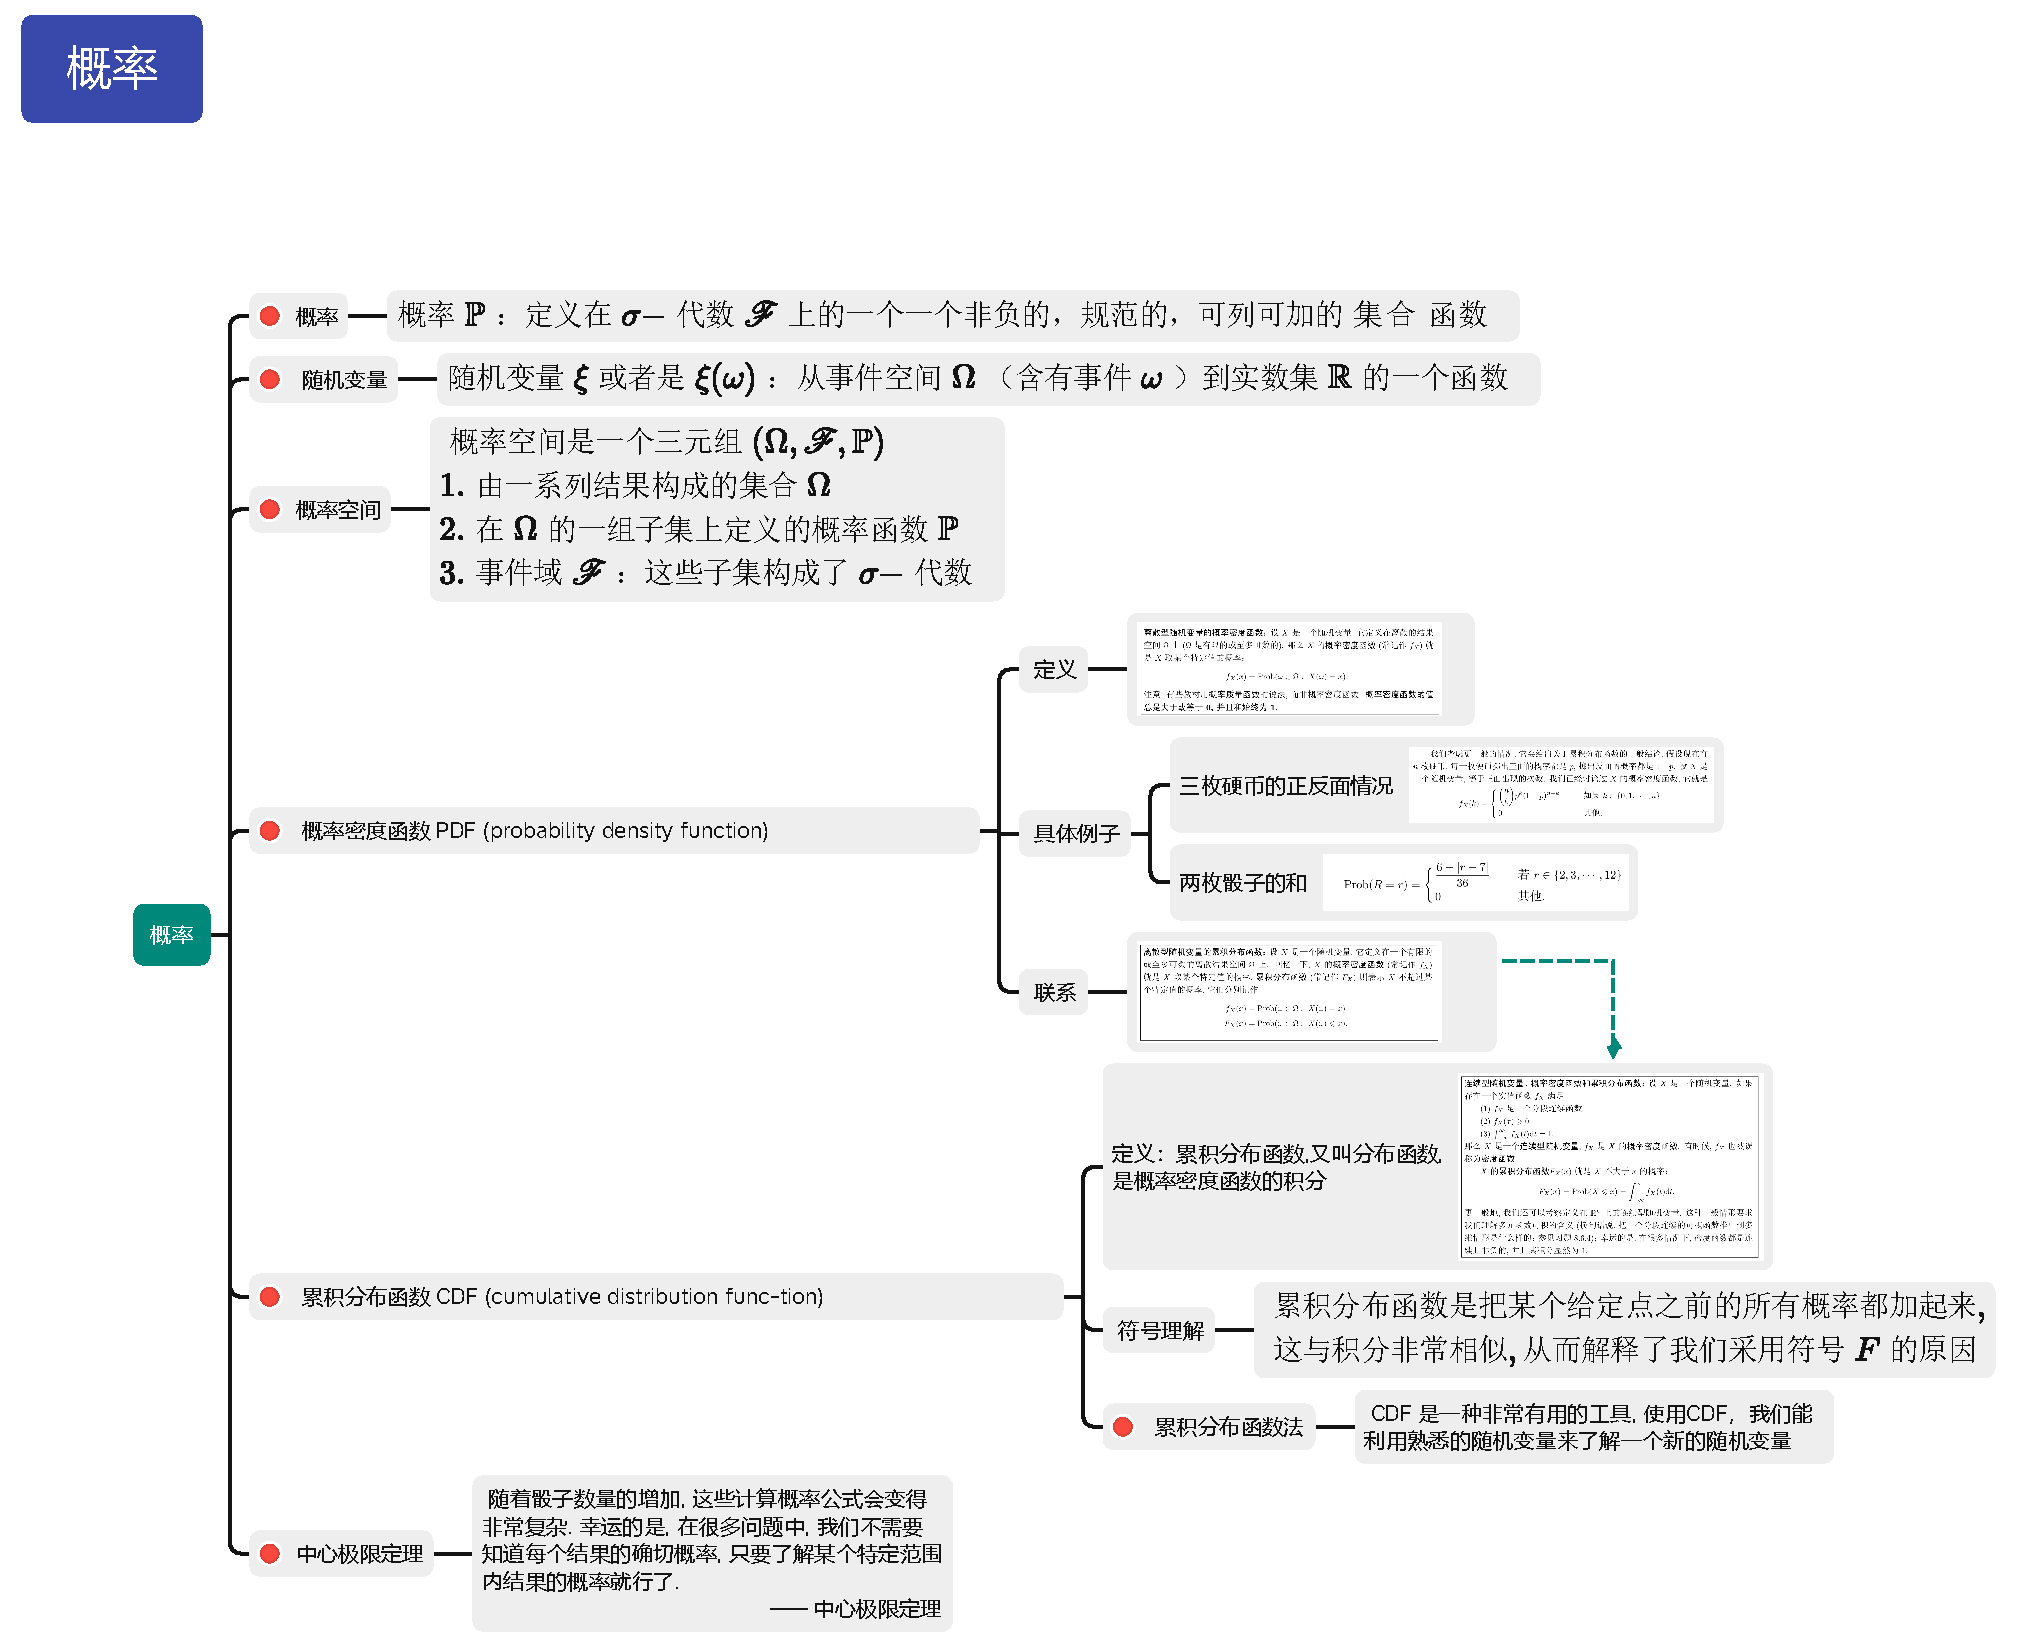
\includegraphics[scale=0.5]{Chapter/TikZ/概率.pdf}
    \label{概率基本对象}
    \caption{概率基本对象}
\end{figure}

\newpage
\section{常见的连续分布}

\begin{definition}[常见的连续分布]
    \num{1}\quad 均匀分布 \hspace*{4em} \num{2}\quad 指数分布
    \hspace*{4em}
    \num{3}\quad 正态分布 \hspace*{4em} \num{4}\quad $\beta$分布
\end{definition}


\noindent\num{1} {\sf 均匀分布}\par

\begin{align}
    \xi \sim \mathrm{U[a, b]}, ~~
    \mathrm{p(X)}=\begin{cases}
        \frac{1}{b-a},&a\le x\le b\\
        0, &\mathtext{其他}
    \end{cases}~~
    \mathrm{F(X)}=\begin{cases}
        0, & x<0\\
        \frac{x-a}{b-a}, &a\le x< b\\
        1,&x\ge b
    \end{cases}
\end{align}

\begin{center}
    \begin{tikzpicture}
        \draw[-stealth] (0, -1) -- (0, 2.5)node[right] {$\mathrm{p(X)}$};
        \draw[-stealth] (-1, 0) -- (6, 0)node[below] {$\mathrm{X}$};
        \node[black, left=8pt, below] at (0, 0) {$O$};
        \draw[red] (-0.3, 0) -- (1, 0);
        \draw[dashed] (1, 1) -- (0, 1);
        \draw[red] (1, 1) -- (2, 1);
        \draw[red] (2, 0) -- (5, 0);
        \node[below, red] at (2, 0) {$b$};
        \node[below, red] at (1, 0) {$a$};
        \draw[dashed, red] (1, 0) -- (1, 1);
        \draw[dashed, red] (2, 0) -- (2, 1);
        \node[left] at (0, 1) {$\frac{1}{b-a}$};
        \draw[fill=black] (0, 1) circle [radius=1pt];
        \draw[draw=black] (1, 0) circle [radius=1pt];
        \draw[draw=black] (2, 0) circle [radius=1pt];
        \node at (3.5, -1) {\mathtext{显然,}$\mathrm{p(X)}$\mathtext{在}$\mathrm{X=a, X=b}$\mathtext{处均不连续。}}; 
    \end{tikzpicture}  
    \begin{tikzpicture}
        \draw[-stealth] (0, -1) -- (0, 2.5)node[right] {$\mathrm{F(X)}$};
        \draw[-stealth] (-1, 0) -- (6, 0)node[below] {$\mathrm{X}$};
        \node[black, left=8pt, below] at (0, 0) {$O$};
        \draw[red] (-0.3, 0) -- (1, 0)node[below] {$a$} -- (2, 1) -- (5, 1);
        \node[below, red] at (2, 0) {$b$};
        \draw[dashed] (2, 0) -- (2, 1) -- (0, 1);
        \node[left] at (0, 1) {$\mathrm{1}$};
        \draw[fill=black] (0, 1) circle [radius=1pt];
        \draw[fill=black] (1, 0) circle [radius=1pt];
        \draw[fill=black] (2, 0) circle [radius=1pt];
        \node at (3.5, -1) {\mathtext{显然,}$\mathrm{F(X)}$\mathtext{在所有点处均连续。}}; 
    \end{tikzpicture}      
\end{center}


\noindent\num{2} {\sf 指数分布}\par
\begin{align}
    \mathtext{记作}\xi \sim \mathrm{Exp}(\lambda),~~p(x)=\begin{cases}
    \lambda e^{-\lambda x},&x>0\\
    0,~~~&x\le0
    \end{cases}~~
    F(x) = \begin{cases}
    1-e^{-\lambda x},~~~x>0\\
    0,~~~x\le0
    \end{cases}
\end{align}

\begin{center}
    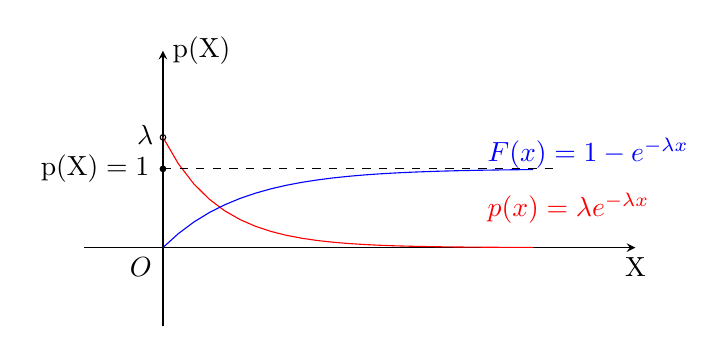
\begin{tikzpicture}
        \draw[-stealth] (0, -1) -- (0, 2.5)node[right] {$\mathrm{p(X)}$};
        \draw[-stealth] (-1, 0) -- (6, 0)node[below] {$\mathrm{X}$};
        \node[black, left=8pt, below] at (0, 0) {$O$};
        \draw[domain=0:4.7, red] plot(\x, {1.4*exp(-1.4*\x)});
        \node[right, red] at (4, 0.5) {$p(x)=\lambda e^{-\lambda x}$};
        \node[left] at (0, 1.43) {$\lambda$};
        \draw (0, 1.4) circle [radius=1pt];
        \draw[domain=0:4.7, blue] plot(\x, {1-exp(-\x)});
        \draw[dashed] (0, 1)node[left, circle, radius=1pt] {$\mathrm{p(X)=1}$} -- (5, 1);
        \draw[fill=black] (0, 1) circle [radius=1pt];
        \node[right, blue] at (4, 1.2) {$F(x)=1- e^{-\lambda x}$};
    \end{tikzpicture}        
\end{center}



设随机变量具有密度函数
\begin{align}
    \Rm{p(x)}=\frac{1}{\sqrt{2\pi}\sigma}\Rm{e}^{-\frac{(x-\mu)^2}{2\sigma^2}},  ~~~-\infty<\rm{x}<+\infty
\end{align}

其中$\mu, \sigma$ 为常数,则称$\xi$服从参数为$\mu, \sigma$的正态分布或Gauss分布,记作$\xi \sim N(\mu, \sigma^2)$.其分布函数为:
\begin{align}
    F(x)=p(\xi \le x)=\int_{-\infty}^{x}{p(y) \dd y}=\frac{1}{\sqrt{2\pi}\sigma} \int_{-\infty}^{x}{\Rm{e}^{-\frac{(y-\mu)^2}{2\sigma^2}} \dd y} , ~~~ -\infty<x<+\infty
\end{align}

\begin{center}
    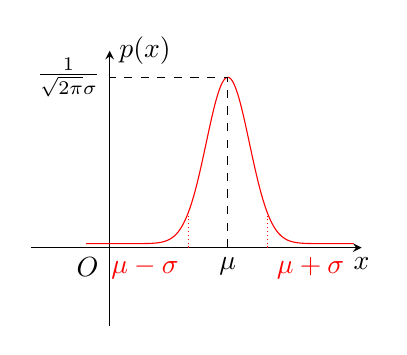
\begin{tikzpicture}
        \draw[-stealth] (0, -1) -- (0, 2.5)node[right] {${p(x)}$};
        \draw[-stealth] (-1, 0) -- (3.2, 0)node[below] {${x}$};
        \node[black, left=8pt, below] at (0, 0) {$O$};
        \draw[domain=-0.3:3.1, red, samples=1000] plot(\x, {1/(sqrt(2*pi))*exp(-(\x-1)*(\x-2)/(0.15))+0.05});
        \draw[dashed] (1.5, 0)node[below] {$\mu$} -- (1.5, 2.16) -- (0, 2.16)node[left] {$\frac{1}{\sqrt{2\pi}\sigma}$};
        \draw[densely dotted, red] (1, 0)node[below left] {$\mu-\sigma$} -- (1, 0.4);
        \draw[densely dotted, red] (2, 0)node[below right] {$\mu+\sigma$} -- (2, 0.4);
    \end{tikzpicture}        
\end{center}



\section{ARMA模型}
\begin{figure}[!htb]
    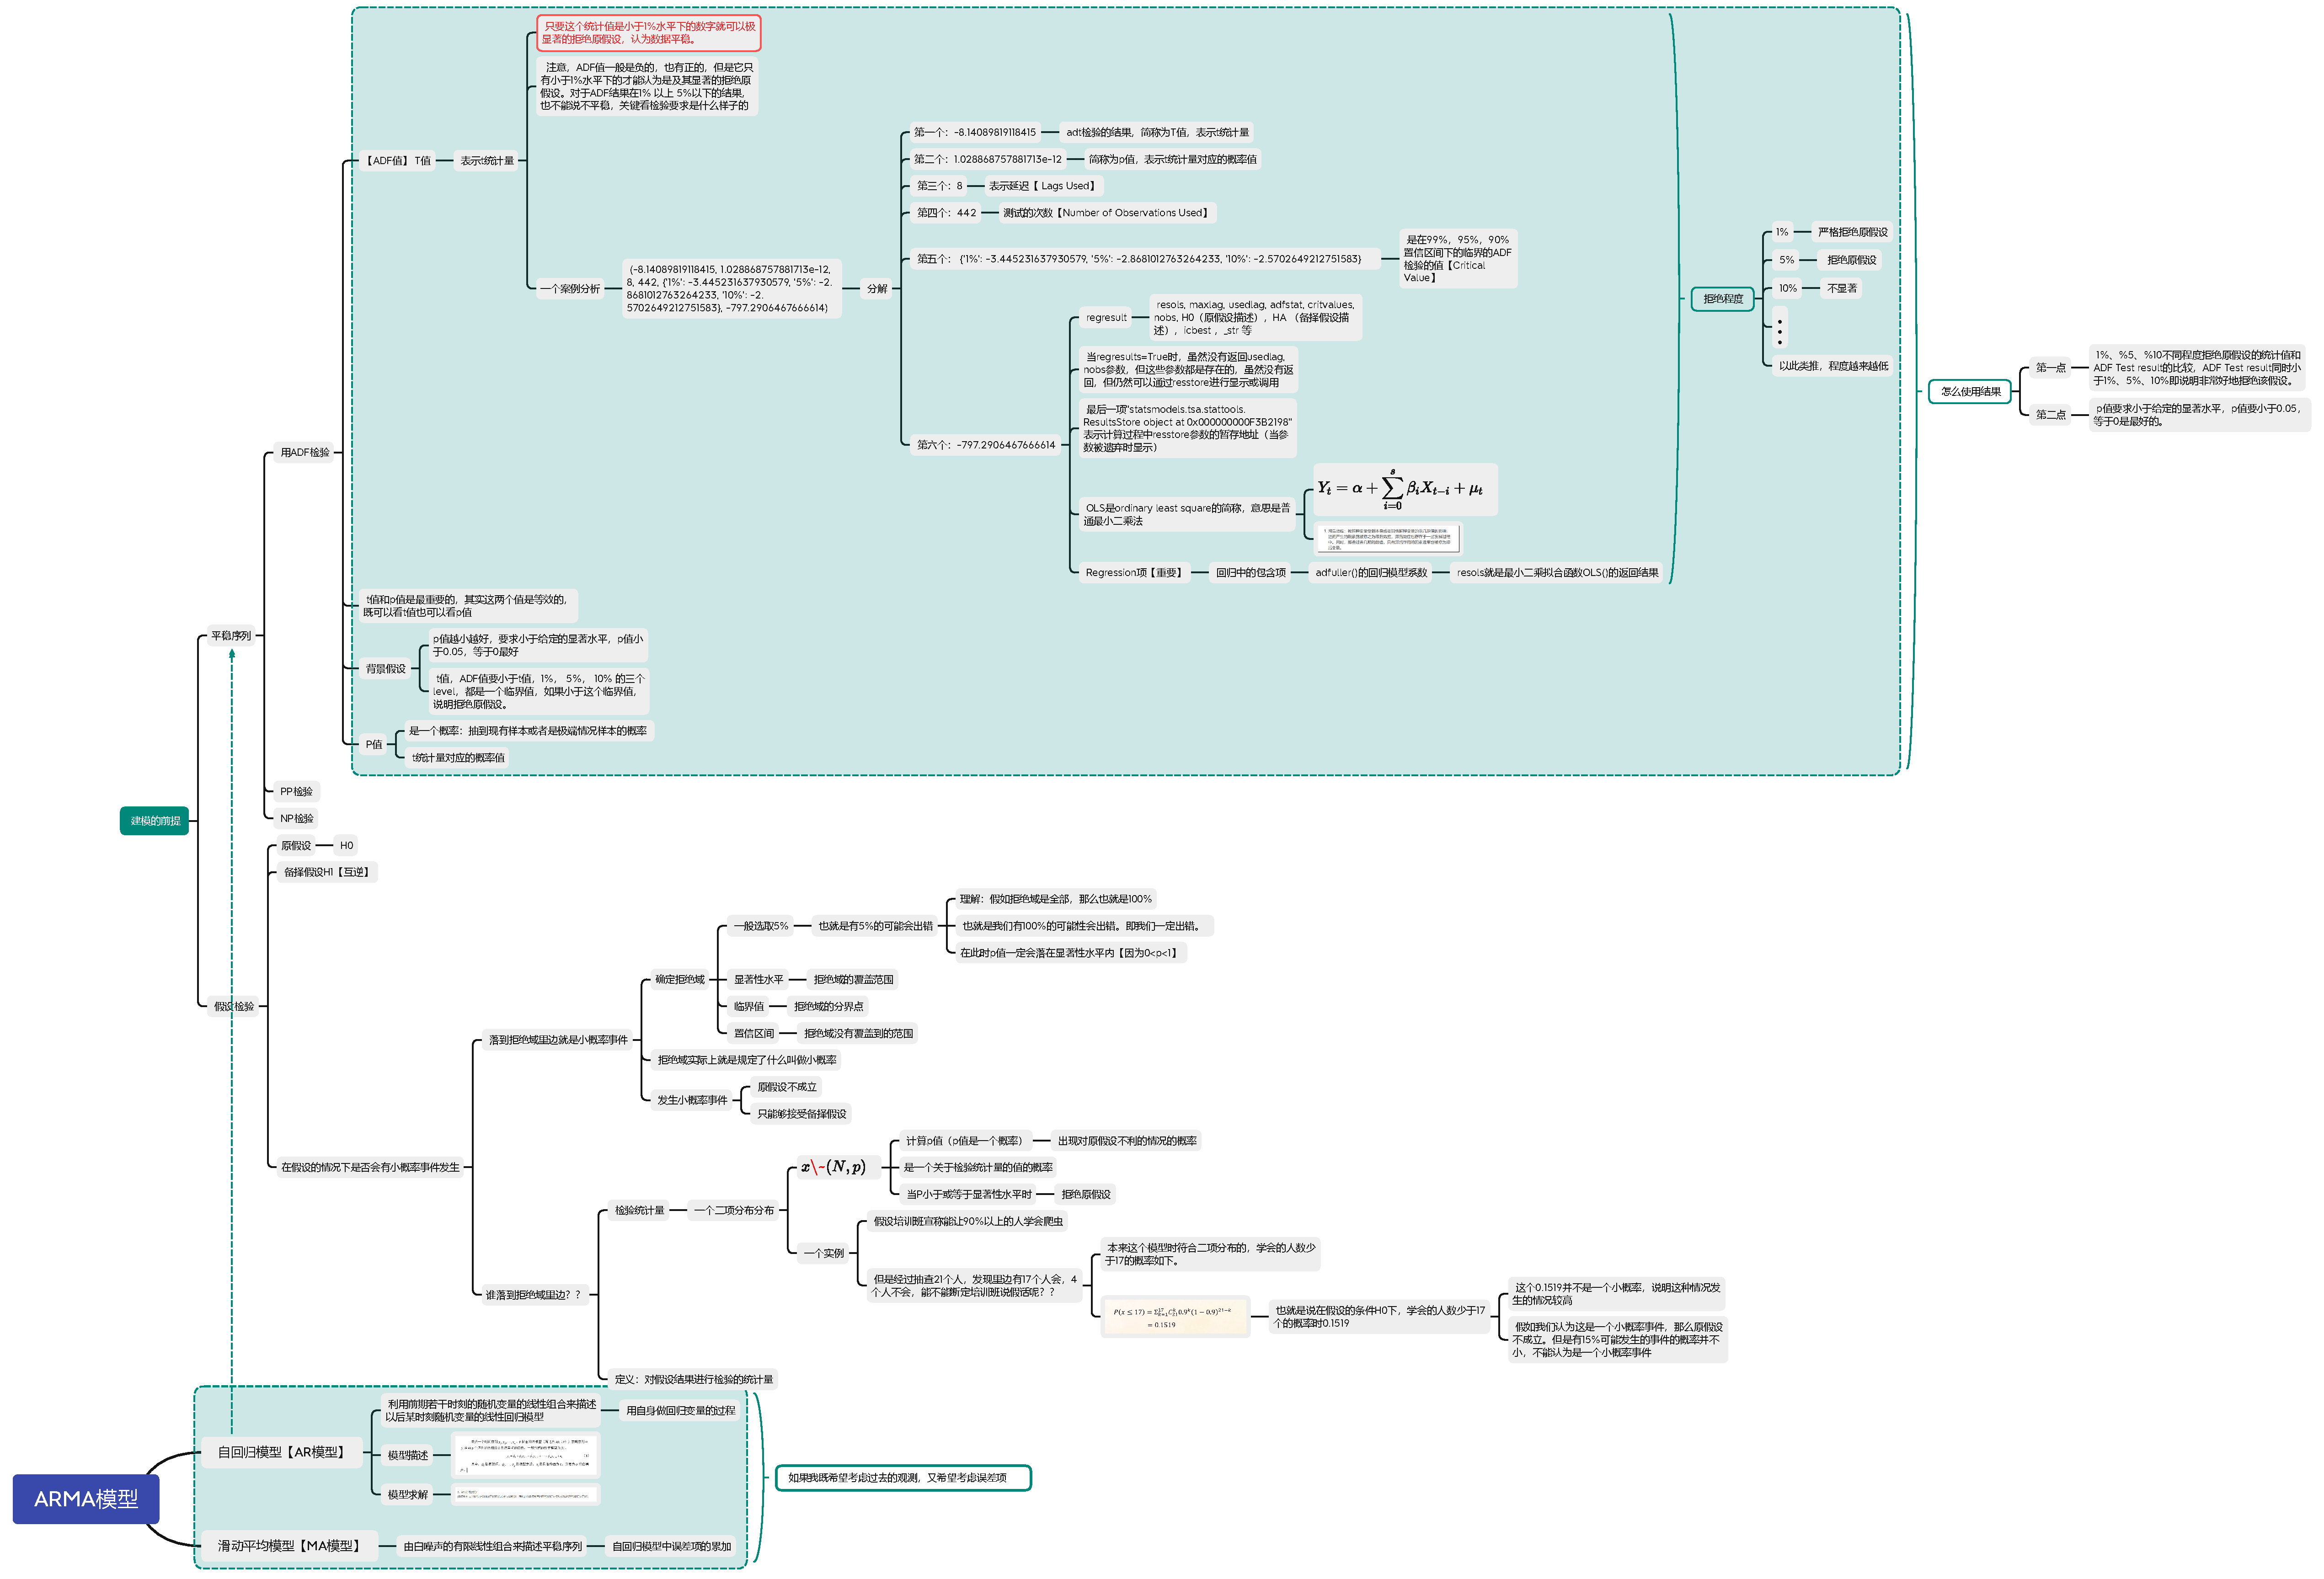
\includegraphics[scale=0.2]{Chapter/TikZ/ARMA模型.pdf}
    \label{ARMA模型}
    \caption{ARMA模型}
\end{figure}


    \chapter{Numerical Analysis}
    \section{向量内积运用}

$\displaystyle  S^*(x)$  是 $f(x)$ 在子集 $\varphi\subset \mathrm{C}[a, b]$中
最佳平方逼近函数

\begin{align*}
    &\biggl(f(x)-S(x),\, f(x)-S(x)\biggr) - \biggl(f(x)-S^*(x),\, f(x)-S^*(x)\biggr) \\
    = & \biggl(f(x)-S^*(x)+S^*(x)-S(x),\, f(x)-S(x)\biggr) - \biggl(f(x)-S^*(x),\, f(x)-S^*(x)\biggr)\\
    = & {\color{blue!40} \biggl(f(x)-S^*(x),\, f(x)-S^*(x)\biggr)} 
        + \biggl(f(x)-S^*(x),\, S^*(x)-S(x)\biggr)
        + \biggl(S^*(x)-S(x),\, f(x)-S^*(x)\biggr)\\
    - & {\color{blue!40} \biggl(f(x)-S^*(x),\, f(x)-S^*(x)\biggr)}
        + {\color{red!40} ||S^*(x)-S(x)||^2 }\\
    = & 2 \biggl(f(x)-S^*(x),\, S^*(x)-S(x)\biggr) + {\color{red!40} ||S^*(x)-S(x)||^2 }
\end{align*}

又因为 
\begin{align*}
    \biggl(f(x),\, \psi_k(x)\biggr) 
    & = \sum_{i=0}^{n}{a_i\biggl(\psi_i(x),\, \psi_k(x)\biggr)}, \quad k = 0, 1, 2, \cdots, n\\
    & = \biggl(\sum_{i=0}^{n}{a_i\psi_i(x)},\, \psi_k(x)\biggr) \\
    & = \biggl(S^*(x),\, \psi_k(x)\biggr)
\end{align*}

于是我们可以得到:
\begin{align}
    \biggl(f(x)-S^*(x),\, \psi_k(x)\biggr) = 0
\end{align}

那么原式就可以化简为:
\begin{align*}
    \mathrm {LHS} 
    & = 2 \biggl(f(x)-S^*(x),\, S^*(x)-S(x)\biggr) + {\color{red!40} ||S^*(x)-S(x)||^2 }\\
    & = 0 + {\color{red!40} ||S^*(x)-S(x)||^2 }\\
    & = {\color{red!40} ||S^*(x)-S(x)||^2 } \\
    & \ge 0  
\end{align*}


于是我们就有:
\begin{align}
    {\bigg|\bigg|f(x)-S^*(x)\bigg|\bigg|^2 \le \bigg|\bigg|f(x) - S(x)\bigg|\bigg|^2} 
\end{align}

    
\end{document}